% Dieses Dokument muss mit PDFLatex gesetzt werden
% Vorteil: Grafiken koennen als jpg, png, ... verwendet werden
%          und die Links im Dokument sind auch gleich richtig
%
%Ermöglicht \\ bei der Titelseite (z.B. bei supervisor)
%Siehe https://github.com/latextemplates/uni-stuttgart-cs-cover/issues/4
\RequirePackage{kvoptions-patch}

%English:
%\let\ifdeutsch\iffalse
%\let\ifenglisch\iftrue

%German:
\let\ifdeutsch\iftrue
\let\ifenglisch\iffalse

%
\ifenglisch
	\PassOptionsToClass{numbers=noenddot}{scrbook}
\else
	%()Aus scrguide.pdf - der Dokumentation von KOMA-Script)
	%Nach DUDEN steht in Gliederungen, in denen ausschließlich arabische Ziffern für die Nummerierung
	%verwendet werden, am Ende der Gliederungsnummern kein abschließender Punkt
	%(siehe [DUD96, R3]). Wird hingegen innerhalb der Gliederung auch mit römischen Zahlen
	%oder Groß- oder Kleinbuchstaben gearbeitet, so steht am Ende aller Gliederungsnummern ein
	%abschließender Punkt (siehe [DUD96, R4])
	\PassOptionsToClass{numbers=autoendperiod}{scrbook}
\fi

%Warns about outdated packages and missing caption delcarations
%See https://www.ctan.org/pkg/nag
\RequirePackage[l2tabu, orthodox]{nag}

%Neue deutsche Trennmuster
%Siehe http://www.ctan.org/pkg/dehyph-exptl und http://projekte.dante.de/Trennmuster/WebHome
%Nur für pdflatex, nicht für lualatex
\RequirePackage{ifluatex}
\ifluatex
%do not load anything
\else
	\ifdeutsch
		\RequirePackage[ngerman=ngerman-x-latest]{hyphsubst}
	\fi
\fi

\documentclass[
               fontsize=12pt, %Default: 11pt, bei Linux Libertine zu klein zum Lesen
% BEGINN: Optionen für typearea
               paper=a4,
               oneside,  % fuer die Betrachtung am Schirm ungeschickt
               BCOR=3mm, % Bindekorrektur
               DIV=13,   % je höher der DIV-Wert, desto mehr geht auf eine Seite. Gute werde sind zwischen DIV=12 und DIV=15
               headinclude=true,
               footinclude=false,
% ENDE: Optionen für typearea
%               titlepage,
               bibliography=totoc,
%               idxtotoc,   %Index ins Inhaltsverzeichnis
%                liststotoc, %List of X ins Inhaltsverzeichnis, mit liststotocnumbered werden die Abbildungsverzeichnisse nummeriert
               headsepline,
               cleardoublepage=empty,
               parskip=half,
%               draft    % um zu sehen, wo noch nachgebessert werden muss - wichtig, da Bindungskorrektur mit drin
               final   % ACHTUNG! - in pagestyle.tex noch Seitenstil anpassen
               ]{scrbook}


%%%
% Beschreibung:
% In dieser Datei werden zuerst die benoetigten Pakete eingebunden und
% danach diverse Optionen gesetzt. Achtung Reihenfolge ist entscheidend!
%
%%%


%%%
% Styleguide:
%
% Ein sehr kleiner Styleguide. Packages werden in Blöcken organisiert.
% Ein Block beginnt mit drei % in einer Zeile, dann % <Blocküberschrift>, dann
% eine Liste der möglichen Optionen und deren Einstellungen, Gründe und Kommentare
% eine % Zeile in der sonst nichts steht und dann wieder %%% in einer Zeile.
%
% Zwischen zwei Blöcken sind 2 Leerzeilen!
% Zu jedem Paket werden soviele Optionen wie möglich/nötig angegeben
%
%%%

%%%
% Codierung
% Wir sind im 21 Jahrhundert, utf-8 löst so viele Probleme.
%
% Mit UTF-8 funktionieren folgende Pakete nicht mehr. Bitte beachten!
%   * fancyvrb mit §
%   * easylist -> http://www.ctan.org/tex-archive/macros/latex/contrib/easylist/
\ifluatex
%no package loading required
\else
\usepackage[utf8]{inputenc}
\fi
%
%%%

%%%
%Parallelbetrieb tex4ht und pdflatex
\makeatletter
\@ifpackageloaded{tex4ht}{\def\iftex4ht{\iftrue}}
                         {\def\iftex4ht{\iffalse}}
\makeatother
%%%


%%%
%Farbdefinitionen
\usepackage[hyperref,dvipsnames]{xcolor}
%

%%%
% Required for custom acronyms/glossaries style
% Left aligned Columns in tables with fixed width
% see http://tex.stackexchange.com/questions/91566/syntax-similar-to-centering-for-right-and-left
\usepackage{ragged2e}
%%%

%%%
% Abkürzungsverzeichnis
\usepackage{scrwfile} % Wichtig, ansonsten erscheint "No room for a new \write"
% siehe http://www.dickimaw-books.com/cgi-bin/faq.cgi?action=view&categorylabel=glossaries#glsnewwriteexceeded
\usepackage[acronym,indexonlyfirst,nomain]{glossaries}
\ifdeutsch
\renewcommand*{\acronymname}{Abkürzungsverzeichnis}
\else
\renewcommand*{\acronymname}{List of Abbreviations}
\fi
\renewcommand*{\glsgroupskip}{}
%
% Removed Glossarie as a table as a quick fix to get the template working again
% see http://tex.stackexchange.com/questions/145579/how-to-print-acronyms-of-glossaries-into-a-table
%
\makenoidxglossaries
%%%


%%%
% Neue deutsche Rechtschreibung und Literatur statt "Literature", Nachfolger von ngerman.sty
\ifdeutsch
% letzte Sprache ist default, Einbindung von "american" ermöglicht \begin{otherlanguage}{amercian}...\end{otherlanguage} oder \foreignlanguage{american}{Text in American}
% see also http://tex.stackexchange.com/a/50638/9075
\usepackage[american,ngerman]{babel}
% Ein "abstract" ist eine "Kurzfassung", keine "Zusammenfassung"
\addto\captionsngerman{%
	\renewcommand\abstractname{Kurzfassung}%
}
\else
%
%
% if you are writing in english
% last language is the default language
\usepackage[ngerman,american]{babel}
\fi
%
%%%

%%%
% Anführungszeichen
% Zitate in \enquote{...} setzen, dann werden automatisch die richtigen Anführungszeichen verwendet.
\usepackage{csquotes}
%%%


%%%
% erweitertes Enumerate
\usepackage{paralist}
%
%%%


%%%
% fancyheadings (nicht nur) fuer koma
\usepackage[automark]{scrlayer-scrpage}
%
%%%


%%%
%Mathematik
%
\usepackage[]{amsmath} % Viele Mathematik-Sachen: Doku: /usr/share/doc/texmf/latex/amsmath/amsldoc.dvi.gz
\PassOptionsToPackage{fleqn,leqno}{amsmath} % options must be passed this way, otherwise it does not work with glossaries
%fleqn (=Gleichungen linksbündig platzieren) funktioniert nicht direkt. Es muss noch ein Patch gemacht werden:
%\addtolength\mathindent{1em}%work-around ams-math problem with align and 9 -> 10. Does not work with glossaries, No visual changes.
\usepackage{mathtools} %fixes bugs in AMS math
%
%for theorems, replacement for amsthm
\usepackage[amsmath,hyperref]{ntheorem}
\theorempreskipamount 2ex plus1ex minus0.5ex
\theorempostskipamount 2ex plus1ex minus0.5ex
\theoremstyle{break}
\newtheorem{definition}{Definition}[section]
%
%%%


%%%
% Intelligentes Leerzeichen um hinter Abkürzungen die richtigen Abstände zu erhalten, auch leere.
% siehe commands.tex \gq{}
\usepackage{xspace}
%Macht \xspace und \enquote kompatibel
\makeatletter
\xspaceaddexceptions{\grqq \grq \csq@qclose@i \} }
\makeatother
%
%%%


%%%
% Anhang
\usepackage{appendix}
%[toc,page,title,header]
%
%%%


%%%
% Grafikeinbindungen
\usepackage{subcaption}
\usepackage{graphicx}%Parameter "pdftex" unnoetig
\graphicspath{{\getgraphicspath}}
\newcommand{\getgraphicspath}{graphics/}
%
%%%


%%%
% Enables inclusion of SVG graphics - 1:1 approach
% This is NOT the approach of http://www.ctan.org/tex-archive/info/svg-inkscape,
% which allows text in SVG to be typeset using LaTeX
% We just include the SVG as is
\usepackage{epstopdf}
\epstopdfDeclareGraphicsRule{.svg}{pdf}{.pdf}{%
  inkscape -z -D --file=#1 --export-pdf=\OutputFile
}
%
%%%


%%%
% Enables inclusion of SVG graphics - text-rendered-with-LaTeX-approach
% This is the approach of http://www.ctan.org/tex-archive/info/svg-inkscape,
\newcommand{\executeiffilenewer}[3]{%
\IfFileExists{#2}
{
%\message{file #2 exists}
\ifnum\pdfstrcmp{\pdffilemoddate{#1}}%
{\pdffilemoddate{#2}}>0%
{\immediate\write18{#3}}
\else
{%\message{file up to date #2}
}
\fi%
}{
%\message{file #2 doesn't exist}
%\message{argument: #3}
%\immediate\write18{echo "test" > xoutput.txt}
\immediate\write18{#3}
}
}
\newcommand{\includesvg}[1]{%
\executeiffilenewer{#1.svg}{#1.pdf}%
{
inkscape -z -D --file=\getgraphicspath#1.svg %
--export-pdf=\getgraphicspath#1.pdf --export-latex}%
\input{\getgraphicspath#1.pdf_tex}%
}


%%%
\usepackage{siunitx}
%%%

%%%
% Tabellenerweiterungen
\usepackage{array} %increases tex's buffer size and enables ``>'' in tablespecs
\usepackage{longtable}
\usepackage{dcolumn} %Aligning numbers by decimal points in table columns
\ifdeutsch
	\newcolumntype{d}[1]{D{.}{,}{#1}}
\else
	\newcolumntype{d}[1]{D{.}{.}{#1}}
\fi

%
%%%

%%%
% Eine Zelle, die sich über mehrere Zeilen erstreckt.
% Siehe Beispieltabelle in Kapitel 2
\usepackage{multirow}
%
%%%

%%%
%Fuer Tabellen mit Variablen Spaltenbreiten
%\usepackage{tabularx}
%\usepackage{tabulary}
%
%%%


%%%
% Links verhalten sich so, wie sie sollen
\usepackage{url}
%
%Use text font as url font, not the monospaced one
%see comments at http://tex.stackexchange.com/q/98463/9075
\urlstyle{same}
%
%Hint by http://tex.stackexchange.com/a/10419/9075
\makeatletter
\g@addto@macro{\UrlBreaks}{\UrlOrds}
\makeatother
%
%%%


%%%
% Index über Begriffe, Abkürzungen
%\usepackage{makeidx} makeidx ist out -> http://xindy.sf.net verwenden
%
%%%

%%%
%lustiger Hack fuer das Abkuerzungsverzeichnis
%nach latex durchlauf folgendes ausfuehren
%makeindex ausarbeitung.nlo -s nomencl.ist -o ausarbeitung.nls
%danach nochmal latex
%\usepackage{nomencl}
%    \let\abk\nomenclature %Deutsche Ueberschrift setzen
%          \renewcommand{\nomname}{List of Abbreviations}
%        %Punkte zw. Abkuerzung und Erklaerung
%          \setlength{\nomlabelwidth}{.2\hsize}
%          \renewcommand{\nomlabel}[1]{#1 \dotfill}
%        %Zeilenabstaende verkleinern
%          \setlength{\nomitemsep}{-\parsep}
%    \makenomenclature
%
%%%

%%%
% Logik für Tex
\usepackage{ifthen} %fuer if-then-else @ commands.tex
%
%%%


%%%
%
\usepackage{listings}
%
%%%


%%%
%Alternative zu Listings ist fancyvrb. Kann auch beides gleichzeitig benutzt werden.
\usepackage{fancyvrb}
%\fvset{fontsize=\small} %Groesse fuer den Fliesstext. Falls deaktiviert: \normalsize
%Funktioniert mit UTF-8 nicht mehr
%\DefineShortVerb{\§} %Somit kann im Text ganz einfach |verbatim| text gesetzt werden.
\RecustomVerbatimEnvironment{Verbatim}{Verbatim}{fontsize=\footnotesize}
\RecustomVerbatimCommand{\VerbatimInput}{VerbatimInput}{fontsize=\footnotesize}
%
%%%


%%%
% Bildunterschriften bei floats genauso formatieren wie bei Listings
% Anpassung wird unten bei den newfloat-Deklarationen vorgenommen
% https://www.ctan.org/pkg/caption2 is superseeded by this package.
\usepackage{caption}
%
%%%


%%%
% Ermoeglicht es, Abbildungen um 90 Grad zu drehen
% Alternatives Paket: rotating Allerdings wird hier nur das Bild gedreht, während bei lscape auch die PDF-Seite gedreht wird.
%Das Paket lscape dreht die Seite auch nicht
\usepackage{pdflscape}
%
%%%


%%%
% Fuer listings
% Wird für fancyvrb und für lstlistings verwendet
\usepackage{float}

%\usepackage{floatrow}
%% zustäzlich für den Paramter [H] = Floats WIRKLICH da wo sie deklariert wurden paltzieren - ganz ohne Kompromisse
% floatrow ist der Nachfolger von float
% Allerdings macht floatrow in manchen Konstellationen Probleme. Deshalb ist das Paket deaktiviert.
%
%%%



%%%
% Fuer Abbildungen innerhalb von Abbildungen
% Ersetzt das Paket subfigure
%
% Due to bug #24 in the caption package we need to update caption3.sty at the moment manualy to use subfig.
% Bug #24: http://sourceforge.net/p/latex-caption/tickets/24/
% corrected caption3.sty: http://sourceforge.net/p/latex-caption/code/HEAD/tree/branches/3.3/tex/caption3.sty
%
%\usepackage[caption=false, lofdepth=1, lotdepth, margin=5pt]{subfig}
%
%%%




%%%
% Fußnoten
%
%\usepackage{dblfnote}  %Zweispaltige Fußnoten
%
% Keine hochgestellten Ziffern in der Fußnote (KOMA-Script-spezifisch):
%\deffootnote[1.5em]{0pt}{1em}{\makebox[1.5em][l]{\bfseries\thefootnotemark}}
%
% Abstand zwischen Fußnoten vergrößern:
%\setlength{\footnotesep}{.85\baselineskip}
%
%
%
%Folgendes Kommando deaktiviert die Trennlinie zur Fußnote
%\renewcommand{\footnoterule}{}
%
\addtolength{\skip\footins}{\baselineskip} % Abstand Text <-> Fußnote
%
% Fußnoten immer ganz unten auf einer \raggedbottom-Seite
% fnpos kommt aus dem yafoot package
\usepackage{fnpos}
\makeFNbelow
\makeFNbottom
%
%%%


%%%
%
\raggedbottom     % Variable Seitenhöhen zulassen
%
%%%


%%%
% Falls die Seitenzahl bei einer Referenz auf eine Abbildung nur dann angegeben werden soll,
% falls sich die Abbildung nicht auf der selben Seite befindet...
\iftex4ht
%tex4ht does not work well with vref, therefore we emulate vref behavior
\newcommand{\vref}[1]{\ref{#1}}
\else
\ifdeutsch
\usepackage[ngerman]{varioref}
\else
\usepackage{varioref}
\fi
\fi
%%%

%%%
% Noch schoenere Tabellen als mit booktabs mit http://www.zvisionwelt.de/downloads.html
\usepackage{booktabs}
%
%\usepackage[section]{placeins}
%
%%%


%%%
%Fuer Graphiken. Allerdings funktioniert es nicht zusammen mit pdflatex
%\usepackage{gastex} % \tolarance kann dann nicht mehr umdefiniert werden
%
%%%


%%%
%
%\usepackage{multicol}
%\usepackage{setspace} % kollidiert mit diplomarbeit.sty
%
%http://www.tex.ac.uk/cgi-bin/texfaq2html?label=floats
%\usepackage{flafter} %floats IMMER nach ihrer Deklaration platzieren
%
%%%


%%%
%schoene TODOs
\usepackage{todonotes}
\let\xtodo\todo
\renewcommand{\todo}[1]{\xtodo[inline,color=black!5]{#1}}
\newcommand{\utodo}[1]{\xtodo[inline,color=green!5]{#1}}
\newcommand{\itodo}[1]{\xtodo[inline]{#1}}
%
%%%


%%%
%biblatex statt bibtex
\usepackage[
  backend       = biber, %biber does not work with 64x versions alternative: bibtex8
						 %minalphanames only works with biber backend
  sortcites     = true,
  bibstyle      = alphabetic,
  citestyle     = alphabetic,
  firstinits    = true,
  useprefix     = false, %"von, van, etc." will be printed, too. See below.
  minnames      = 1,
  minalphanames = 3,
  maxalphanames = 4,
  maxbibnames   = 99,
  maxcitenames  = 3,
	natbib        = true,
	eprint        = true,
	url           = true,
  doi           = false,
  isbn          = true,
  backref       = false]{biblatex}
\bibliography{bibliography}
%\addbibresource[datatype=bibtex]{bibliography.bib}

%Do not put "vd" in the label, but put it at "\citeauthor"
%Source: http://tex.stackexchange.com/a/30277/9075
\makeatletter
\AtBeginDocument{\toggletrue{blx@useprefix}}
\AtBeginBibliography{\togglefalse{blx@useprefix}}
\makeatother

%Thin spaces between initials
%http://tex.stackexchange.com/a/11083/9075
\renewrobustcmd*{\bibinitdelim}{\,}

%Keep first and last name together in the bibliography
%http://tex.stackexchange.com/a/196192/9075
\renewcommand*\bibnamedelimc{\addnbspace}
\renewcommand*\bibnamedelimd{\addnbspace}

%Replace last "and" by comma in bibliography
%See http://tex.stackexchange.com/a/41532/9075
\AtBeginBibliography{%
  \renewcommand*{\finalnamedelim}{\addcomma\space}%
}

\DefineBibliographyStrings{ngerman}{
  backrefpage  = {zitiert auf S\adddot},
  backrefpages = {zitiert auf S\adddot},
  andothers    = {et\ \addabbrvspace al\adddot},
  %Tipp von http://www.mrunix.de/forums/showthread.php?64665-biblatex-Kann-%DCberschrift-vom-Inhaltsverzeichnis-nicht-%E4ndern&p=293656&viewfull=1#post293656
  bibliography = {Literaturverzeichnis}
}

%enable hyperlinked author names when using \citeauthor
%source: http://tex.stackexchange.com/a/75916/9075
\DeclareCiteCommand{\citeauthor}
  {\boolfalse{citetracker}%
   \boolfalse{pagetracker}%
   \usebibmacro{prenote}}
  {\ifciteindex
     {\indexnames{labelname}}
     {}%
   \printtext[bibhyperref]{\printnames{labelname}}}
  {\multicitedelim}
  {\usebibmacro{postnote}}

%natbib compatibility
%\newcommand{\citep}[1]{\cite{#1}}
%\newcommand{\citet}[1]{\citeauthor{#1} \cite{#1}}
%Beginning of sentence - analogous to cleveref - important for names such as "zur Muehlen"
%\newcommand{\Citep}[1]{\cite{#1}}
%\newcommand{\Citet}[1]{\Citeauthor{#1} \cite{#1}}
%%%


%%%
% Blindtext. Paket "blindtext" ist fortgeschritterner als "lipsum" und kann auch Mathematik im Text (http://texblog.org/2011/02/26/generating-dummy-textblindtext-with-latex-for-testing/)
% kantlipsum (https://www.ctan.org/tex-archive/macros/latex/contrib/kantlipsum) ist auch ganz nett, aber eben auch keine Mathematik
% Wird verwendet, um etwas Text zu erzeugen, um eine volle Seite wegen Layout zu sehen.
\usepackage[math]{blindtext}
%%%

%%%
% Neue Pakete bitte VOR hyperref einbinden. Insbesondere bei Verwendung des
% Pakets "index" wichtig, da sonst die Referenzierung nicht funktioniert.
% Für die Indizierung selbst ist unter http://xindy.sourceforge.net
% ein gutes Tool zu erhalten
%%%


%%%
%
% hier also neue packages einbinden
%
%%%



\usepackage{pdfpages}
%nice linebreaks in table
\usepackage{multicol}
\usepackage{tabularx}


%%%
% ggf.in der Endversion komplett rausnehmen. dann auch \href in commands.tex aktivieren
% Alle Optionen nach \hypersetup verschoben, sonst crash
%
\usepackage[]{hyperref}%siehe auch: "Praktisches LaTeX" - www.itp.uni-hannover.de/~kreutzm
%
%% Da es mit KOMA 3 und xcolor zu Problemen mit den global Options kommt MÜSSEN die Optionen so gesetzt werden.
%

% Eigene Farbdefinitionen ohne die Namen des xcolor packages
\definecolor{darkblue}{rgb}{0,0,.5}
\definecolor{black}{rgb}{0,0,0}

\hypersetup{
    breaklinks=true,
    bookmarksnumbered=true,
    bookmarksopen=true,
    bookmarksopenlevel=1,
    breaklinks=true,
    colorlinks=true,
    pdfstartview=Fit,
    pdfpagelayout=TwoPageRight, % zweiseitige Darstellung: ungerade Seiten rechts im PDF-Viewer - siehe auch http://tex.stackexchange.com/a/21109/9075
    filecolor=darkblue,
    urlcolor=darkblue,
    linkcolor=black,
    citecolor=black
}
%
%%%


%%%
% cleveref für cref statt autoref, da cleveref auch bei Definitionen funktioniert
\ifdeutsch
\usepackage[ngerman,capitalise,nameinlink,noabbrev]{cleveref}
\else
\usepackage[capitalise,nameinlink,noabbrev]{cleveref}
\fi
%%%


%%%
% Zur Darstellung von Algorithmen
% Algorithm muss nach hyperref geladen werden
\usepackage[chapter]{algorithm}
\usepackage[]{algpseudocode}
%
%%%


%%%
% Schriften
%%%
%
\automark[section]{chapter}
\ifenglisch
%serif font also in heading, foot and page number (contained in foot)
\setkomafont{pageheadfoot}{\normalfont\rmfamily}
\setkomafont{pagenumber}{\normalfont\rmfamily}
\else
%sans serif font in German texts
\setkomafont{pageheadfoot}{\normalfont\sffamily}
\setkomafont{pagenumber}{\normalfont\sffamily}
\fi
%
%\setheadsepline[.4pt]{.4pt} %funktioniert nicht: Alle Linien sind hier weg
%
%%%

%%%
%
\ifenglisch
% Fuer englische Texte sind serifenhafte Ueberschriften gut. Deshalb hier der Befehl zum Aktivieren von serifenhaften Ueberschriften
\setkomafont{disposition}{\normalfont\rmfamily}

% Bei englischen Texten das Label (optionaler Eintrag bei \item) bei description-Umgegungen nur auf fett und nicht fett+serifenlos stellen.
\setkomafont{descriptionlabel}{\normalfont\bfseries}
\fi
%
%%%

%%%
% Fuer deutsche Texte: Weniger Silbentrennung, mehr Abstand zwischen den Woertern
\ifdeutsch
\setlength{\emergencystretch}{3em} % Silbentrennung reduzieren durch mehr frei Raum zwischen den Worten
\fi
%%%

%Symbole
%--------
%\usepackage[geometry]{ifsym} % \BigSquare
%\usepackage{mathabx}
%\usepackage{stmaryrd} %fuer \ovee, \owedge, \otimes
%\usepackage{marvosym} %fuer \Writinghand %patched to not redefine \Rightarrow
%\usepackage{mathrsfs} %mittels \mathscr{} schoenen geschwungenen Buchstaben erzeugen
%\usepackage{calrsfs} %\mathcal{} ein bisserl dickeren buchstaben erzeugen - sieht net so gut aus.
                      %durch mathpazo ist das schon definiert
\usepackage{amssymb}

%For \texttrademark{}
\usepackage{textcomp}

%name-clashes von marvosym und mathabx vermeiden:
\def\delsym#1{%
%  \expandafter\let\expandafter\origsym\expandafter=\csname#1\endcsname
%  \expandafter\let\csname orig#1\endcsname=\origsym
  \expandafter\let\csname#1\endcsname=\relax
}

%\usepackage{pifont}
%\usepackage{bbding}
%\delsym{Asterisk}
%\delsym{Sun}\delsym{Mercury}\delsym{Venus}\delsym{Earth}\delsym{Mars}
%\delsym{Jupiter}\delsym{Saturn}\delsym{Uranus}\delsym{Neptune}
%\delsym{Pluto}\delsym{Aries}\delsym{Taurus}\delsym{Gemini}
%\delsym{Rightarrow}
%\usepackage{mathabx} - Ueberschreibt leider zu viel - und die \le-Zeichen usw. sehen nicht gut aus!


%Fallback-Schriftart
\usepackage{lmodern}  % Latin Modern Fonts sind die Nachfolger von Computer Modern, den LaTeX-Standardfonts
%Quelle: http://homepage.ruhr-uni-bochum.de/Georg.Verweyen/pakete.html
%Allerdings sieht diese Schritart in Diplomarbeiten fuer Fliesstext auch nicht besonders schoen aus.
%Trotzdem ist sie fuer Programmcode gut geeignet

%Schriftart fuer die Ueberschriften - ueberschreibt lmodern
\ifdeutsch
\usepackage[scaled=.95]{helvet}
\else
\usepackage[scaled=.90]{helvet}
\fi

% Für Schreibschrift würde tun, muss aber ned
%\usepackage{mathrsfs} %  \mathscr{ABC}

%Schriftart fuer den Fliesstext - ueberschreibt lmodern
%
\ifdeutsch
%
%Linux Libertine, siehe http://www.linuxlibertine.org/
%Packageparamter [osf] = Minuskel-Ziffern
%rm = libertine im Brottext, Linux Biolinum NICHT als serifenlose Schrift, sondern helvet (von oben) beibehalten
\usepackage[rm]{libertine}
%
%Alternative Schriftart: Palantino, Packageparamter [osf] = Minuskel-Ziffern
%\usepackage{mathpazo} %ftp://ftp.dante.de/tex-archive/fonts/mathpazo/ - Tipp aus DE-TEX-FAQ 8.2.1
%
\fi

\ifenglisch
%
\usepackage{charter} %Charter fuer englische Texte
\linespread{1.05} % Durchschuss für Charter leicht erhöhen
%
%\usepackage{mathptmx} %Times fuer englische Texte. Sieht nicht sooo gut aus.
%
%Fallback ist lmodern, die oben eingebunden wurde
\fi

%Schriftart fuer Programmcode - ueberschreibt lmodern
%Falls auskommentiert, wird die Standardschriftart lmodern genommen
%\usepackage[scaled=.92]{luximono} % Fuer schreibmaschinenartige Schluesselwoerter in den Listings - geht bei alten Installationen nicht, da einige Fontshapes (<>=) fehlen
%\usepackage{courier}
\usepackage[scaled=0.83]{beramono} %BeraMono als Typewriter-Schrift, Tipp von http://tex.stackexchange.com/a/71346/9075

\ifluatex
\else
\usepackage[T1]{fontenc}
\fi


% optischer Randausgleich - bei miktex gleich dabei - bei linux von
%  http://www.ctan.org/tex-archive/macros/latex/contrib/microtype/
%  herunterladen 
\usepackage{microtype}
%Falls bei einer Silbentrennung ploetzlich eine ganze Zeile fehlt (passiert unter Windows XP mit MikTex 2.5 und foxit reader als pdfreader
%\usepackage{pdfcprot}
%ausprobieren. Dieses erzeugt allerdings nur für Palatino (in dieser Vorlage die Default-Schrift) einen guten optischen Randausgleich
%Falls alle Stricke reissen, muss leider auf den optischen Randausgleich verzichtet werden.

%fuer microtype
%tracking=true muss als Parameter des microtype-packages mitgegeben werden
%
%Deaktiviert, da dies bei Algorithmen seltsam aussieht
%
%\DeclareMicrotypeSet*[tracking]{my}{ font = */*/*/sc/* }% 
%\SetTracking{ encoding = *, shape = sc }{ 45 }% Hier wird festgelegt,
            % dass alle Passagen in Kapitälchen automatisch leicht
            % gesperrt werden.
			% Quelle: http://homepage.ruhr-uni-bochum.de/Georg.Verweyen/pakete.html

%
%%%


%%%
% Links auf Gleitumgebungen springen nicht zur Beschriftung,
% Doc: http://mirror.ctan.org/tex-archive/macros/latex/contrib/oberdiek/hypcap.pdf
% sondern zum Anfang der Gleitumgebung
\usepackage[all]{hypcap}
%%%


%%%
% Deckblattstyle
%
\ifdeutsch
	\PassOptionsToPackage{language=german}{uni-stuttgart-cs-cover}
\else
	\PassOptionsToPackage{language=english}{uni-stuttgart-cs-cover}
\fi

\usepackage[
    title={Förderungswürdigkeit der F\"{o}rderung von Öl},
    author={Lars K.},
    type=bachelor,
    institute=iaas,
    number=12345,
    course=se,
    examiner={Prof.\ Dr.\ Uwe Fessor},
    supervisor={Dipl.-Inf.\ Roman Tiker,\\Dipl.-Inf.\ Laura Stern,\\Otto Normalverbraucher,\ M.Sc.},
    startdate={5.\ Juli 2013}, % English: July 5, 2013;    ISO: 2013-07-05
    enddate={5.\ Januar 2014}, % English: January 5, 2014; ISO: 2014-01-05
    crk={I.7.2}
    ]{uni-stuttgart-cs-cover}
%
%%%


%%%
%Bugfixes packages
%\usepackage{fixltx2e} %Fuer neueste LaTeX-Installationen nicht mehr benoetigt - bereinigte einige Ungereimtheiten, die auf Grund von Rueckwaertskompatibilitaet beibahlten wurden.
%\usepackage{mparhack} %Fixt die Position von marginpars (die in DAs selten bis gar nicht gebraucht werden}
%\usepackage{ellipsis} %Fixt die Abstaende vor \ldots. Wird wohl auch nicht benoetigt.
%
%%%


%%%
% Rand
%Viele Moeglichkeiten, die Raender im Dokument einzustellen.
%Satzspiegel neu berechnen. Dokumentation dazu ist in "scrguide.pdf" von KOMA-Skript zu finden
%  Optionen werden bei \documentclass[] in ausarbeitung.tex mitgegeben.
\typearea[current]{current} %neu berechnen, da neue Schrift eingebunden

%\usepackage{a4}
%\usepackage{a4wide}
%\areaset{170mm}{277mm} %a4:29,7hochx21mbreit

%Wer die Masse direkt eingeben moechte:
%Bei diesem Beispiel wird die Regel nicht beachtet, dass der innere Rand halb so gross wie der aussere Rand und der obere Rand halb so gross wie der untere Rand sein sollte
%\usepackage[inner=2.5cm, outer=2.5cm, includefoot, top=3cm, bottom=1.5cm]{geometry}



%
%%%


%%%
% Optionen
%
\captionsetup{
  format=hang,
  labelfont=bf,
  justification=justified,
  %single line captions should be centered, multiline captions justified
  singlelinecheck=true
}
%
%neue float Umgebung fuer Listings, die mittels fancyvrb gesetzt werden sollen
\floatstyle{ruled}
\newfloat{Listing}{tbp}{code}[chapter]
\crefname{Listing}{Listing}{Listings}
\newfloat{Algorithmus}{tbp}{alg}[chapter]
\ifdeutsch
\crefname{Algorithmus}{Algorithmus}{Algorithmus}
\else
\crefname{Algorithmus}{Algorithm}{Algorithms}
\fi
%
%amsmath
%\numberwithin{equation}{section}
%\renewcommand{\theequation}{\thesection.\Roman{equation}}
%
%pdftex
\pdfcompresslevel=9
%
%Tabellen (array.sty)
\setlength{\extrarowheight}{1pt}
%
%
%%%

%%%
% unterschiedliche Chapter-Styles
% u.a. Paket fncychap
% Andere Kapitelueberschriften
% falls einem der Standard von KOMA nicht gefaellt...
% Falls man zurück zu KOMA moechte, dann muss jede der vier folgenden Moeglichkeiten deaktiviert sein.

% 1. Moeglichkeit
%\usepackage[Sonny]{fncychap}
%oder
%\usepackage[Bjarne]{fncychap}
%oder
%\usepackage[Lenny]{fncychap}

% 2. Moeglichkeit
\iffalse
\usepackage[Bjarne]{fncychap}
\ChNameVar{\Large\sf} \ChNumVar{\Huge} \ChTitleVar{\Large\sf}
\ChRuleWidth{0.5pt} \ChNameUpperCase
\fi

%Variante der 2. Moeglichkeit
\iffalse
\usepackage[Rejne]{fncychap}
\ChNameVar{\centering\Huge\rm\bfseries}
\ChNumVar{\Huge}
 \ChTitleVar{\centering\Huge\rm}
\ChNameUpperCase
\ChTitleUpperCase
\ChRuleWidth{1pt}
\fi

% 3. Moeglichkeit
\iffalse
\usepackage{fncychap}
\ChNameUpperCase
\ChTitleUpperCase
\ChNameVar{\raggedright\normalsize} %\rm
\ChNumVar{\bfseries\Large}
\ChTitleVar{\raggedright\Huge}
\ChRuleWidth{1pt}
\fi

% 4. Moeglichkeit
% Zur Aktivierierung "\iffalse" und "\fi" auskommentieren
% Innen drin kann man dann noch zwischen
%   * serifenloser Schriftart (eingestellt)
%   * serifenhafter Schriftart (wenn kein zusaetzliches Kommando aktiviert ist) und
%   * Kapitälchen wählen
\iffalse
\makeatletter
%\def\thickhrulefill{\leavevmode \leaders \hrule height 1ex \hfill \kern \z@}

%Fuer Kapitel mit Kapitelnummer
\def\@makechapterhead#1{%
  \vspace*{10\p@}%
  {\parindent \z@ \raggedright \reset@font
			%Default-Schrift: Serifenhaft (gut fuer englische Dokumente)
            %A) Fuer serifenlose Schrift:
            \fontfamily{phv}\selectfont
			%B) Fuer Kapitaelchen:
			%\fontseries{m}\fontshape{sc}\selectfont
            %C) Fuer ganz "normale" Schrift:
            %\normalfont 
			%
			\Large \@chapapp{} \thechapter
        \par\nobreak\vspace*{10\p@}%
        \interlinepenalty\@M
    {\Huge\bfseries\baselineskip3ex
	%Fuer Kapitaelchen folgende Zeile aktivieren:
	%\fontseries{m}\fontshape{sc}\selectfont
	#1\par\nobreak}
    \vspace*{10\p@}%
\makebox[\textwidth]{\hrulefill}%    \hrulefill alone does not work
    \par\nobreak
    \vskip 40\p@
  }}

  %Fuer Kapitel ohne Kapitelnummer (z.B. Inhaltsverzeichnis)
  \def\@makeschapterhead#1{%
  \vspace*{10\p@}%
  {\parindent \z@ \raggedright \reset@font
            \normalfont \vphantom{\@chapapp{} \thechapter}
        \par\nobreak\vspace*{10\p@}%
        \interlinepenalty\@M
    {\Huge \bfseries %
	%Default-Schrift: Serifenhaft (gut fuer englische Dokumente)
    %A) Fuer serifenlose Schrift folgende Zeile aktivieren:
    \fontfamily{phv}\selectfont
	%B) Fuer Kapitaelchen folgende Zeile aktivieren:
	%\fontseries{m}\fontshape{sc}\selectfont
	#1\par\nobreak}
    \vspace*{10\p@}%
\makebox[\textwidth]{\hrulefill}%    \hrulefill does not work
    \par\nobreak
    \vskip 40\p@
  }}
%
\makeatother
\fi

%%%

%%%
%Minitoc-Einstellungen
%\dominitoc
%\renewcommand{\mtctitle}{Inhaltsverzeichnis dieses Kapitels}
%
% Disable single lines at the start of a paragraph (Schusterjungen)
\clubpenalty = 10000
%
% Disable single lines at the end of a paragraph (Hurenkinder)
\widowpenalty = 10000 \displaywidowpenalty = 10000
%
%http://groups.google.de/group/de.comp.text.tex/browse_thread/thread/f97da71d90442816/f5da290593fd647e?lnk=st&q=tolerance+emergencystretch&rnum=5&hl=de#f5da290593fd647e
%Mehr Infos unter http://www.tex.ac.uk/cgi-bin/texfaq2html?label=overfull
\tolerance=2000
\setlength{\emergencystretch}{3pt}   % kann man evtl. auf 20 erhoehen
\setlength{\hfuzz}{1pt}
%
%%%


%%%
% Fuer listings.sty
\lstset{language=XML,
        showstringspaces=false,
        extendedchars=true,
        basicstyle=\footnotesize\ttfamily,
        commentstyle=\slshape,
        stringstyle=\ttfamily, %Original: \rmfamily, damit werden die Strings im Quellcode hervorgehoben. Zusaetzlich evtl.: \scshape oder \rmfamily durch \ttfamily ersetzen. Dann sieht's aus, wie bei fancyvrb
        breaklines=true,
        breakatwhitespace=true,
        columns=flexible,
        aboveskip=0mm, %deaktivieren, falls man lstlistings direkt als floating object benutzt (\begin{lstlisting}[float,...])
        belowskip=0mm, %deaktivieren, falls man lstlistings direkt als floating object benutzt (\begin{lstlisting}[float,...])
        captionpos=b
}
\ifdeutsch
\renewcommand{\lstlistlistingname}{Verzeichnis der Listings}
\fi
%
%%%


%%%
%fuer algorithm.sty: - falls Deutsch und nicht Englisch. Falls Englisch als Sprache gewählt wurde, bitte die folgenden beiden Zeilen auskommentieren.
\floatname{algorithm}{Algorithmus}
\ifdeutsch
\renewcommand{\listalgorithmname}{Verzeichnis der Algorithmen}
\fi
%
%%%


%%%
% Das Euro Zeichen
% Fuer Palatino (mathpazo.sty): richtiges Euro-Zeichen
% Alternative: \usepackage{eurosym}
\newcommand{\EUR}{\ppleuro}
%
%%%


%%%
%
% Float-placements - http://dcwww.camd.dtu.dk/~schiotz/comp/LatexTips/LatexTips.html#figplacement
% and http://people.cs.uu.nl/piet/floats/node1.html
\renewcommand{\topfraction}{0.85}
\renewcommand{\bottomfraction}{0.95}
\renewcommand{\textfraction}{0.1}
\renewcommand{\floatpagefraction}{0.75}
%\setcounter{totalnumber}{5}
%
%%%

%%%
%
% Bei Gleichungen nur dann die Nummer zeigen, wenn die Gleichung auch referenziert wird
%
% Funktioniert mit MiKTeX Stand 2012-01-13 nicht. Deshalb ist dieser Schalter deaktiviert.
%
%\mathtoolsset{showonlyrefs}
%
%%%


%%%
%ensure that floats covering a whole page are placed at the top of the page
%see http://tex.stackexchange.com/a/28565/9075
\makeatletter
\setlength{\@fptop}{0pt}
\setlength{\@fpbot}{0pt plus 1fil}
\makeatother
%%%


%%%
%Optischer Randausgleich
\usepackage{microtype}
%%%

%%%
%Package geometry to enlarge on page
%
%Source: http://www.howtotex.com/tips-tricks/change-margins-of-a-single-page/
%
%Normally, this should not be used as the typearea package calculates the margins perfectly
\usepackage[
  pass %just load the package and do not destory the work of typearea
]{geometry}
%%%

%%%
% footnotes in tables
\usepackage{footnote}
\makesavenoteenv{tabular}
\makesavenoteenv{tabularx}
\makesavenoteenv{table}
% Reuse of footnotes
% Reuse of Footnotes, see http://tex.stackexchange.com/questions/10102/multiple-references-to-the-same-footnote-with-hyperref-support-is-there-a-bett
\crefformat{footnote}{#2\footnotemark[#1]#3}
%%%

%Der untere Rand darf "flattern"
\raggedbottom

%%%
% Wie tief wird das Inhaltsverzeichnis aufgeschlüsselt
% 0 --\chapter
% 1 --\section % fuer kuerzeres Inhaltsverzeichnis verwenden - oder minitoc benutzen
% 2 --\subsection
% 3 --\subsubsection
% 4 --\paragraph
\setcounter{tocdepth}{1}
%
%%%

\makeindex

%Angaben in die PDF-Infos uebernehmen
\makeatletter
\hypersetup{
            pdftitle={Studienarbeit T3100}, %Titel der Arbeit
            pdfauthor={Markus Rein}, %Author
            pdfkeywords={}, % CR-Klassifikation und ggf. weitere Stichworte
            pdfsubject={}
}
\makeatother

\newacronym{hil}{HIL}{Hardware-In-the-Loop}
\newacronym{imu}{IMU}{Inertial Measurement Unit}
\newacronym{uas}{UAS}{Unmanned Aircraft System}
\newacronym{uav}{UAV}{Unmanned Aerial Vehicle}
\newacronym{gps}{GPS}{Global Positioning System}
\newacronym{rpi}{RPI}{Raspberry Pi (Einplatinencomputer)}
\newacronym{tcp}{TCP}{Transmission Control Protocol}
\newacronym{udp}{UDP}{User Datagram Protocol}
\newacronym{gcs}{GCS}{Ground Control Station}
\newacronym{ram}{RAM}{Arbeitsspeicher}
\newacronym{lba}{LBA}{Luftfahrt-Bundesamt}
\newacronym{gui}{GUI}{Graphical User Interface}
\newacronym{fps}{FPS}{Frames per Second}
\newacronym{usb}{USB}{Universal Serial Bus}
\newacronym{wlan}{WLAN}{Wireless LAN}
\newacronym{uart}{UART}{Universal Asynchronous Receiver Transmitter}
\newacronym{roi}{ROI}{Region Of Interest}
\newacronym{i2c}{I\textsuperscript{2}C}{Inter-Integrated Circuit}
\newglossaryentry{csv}
{
    name=CSV,
    short={CSV},
    description={Comma Separated Values, Textdatei mit Tabelleninhalt}
}
\newglossaryentry{slam}
{
    name=SLAM,
    short={SLAM},
    description={Simultane Lokalisierung und Kartierung der Umgebung}
}
\newglossaryentry{px4}
{
    name=Pixhawk® 4,
    short=PX4,
    description={Microcontroller, mit Software und Peripherie zur Flugsteuerung}
}
\newglossaryentry{ros}
{
    name=ROS,
    short=ROS,
    description={Robot Operating System, Framework mit Schnittstellen für Sensor/Aktor-Verknüpfungen}
}
\newglossaryentry{mav}
{
    name=MAVLink,
    short=MAVLink,
    description={Binäres Übertragungsprotokoll für ressourcenbeschränkte Umgebungen, bevorzugt auf Robotern und Drohnen eingesetzt}
}


\begin{document}

%tex4ht-Konvertierung verschönern
\iftex4ht
% tell tex4ht to create picures also for formulas starting with '$'
% WARNING: a tex4ht run now takes forever!
\Configure{\$}{\PicMath}{\EndPicMath}{} 
%$ % <- syntax highlighting fix for emacs
\Css{body {text-align:justify;}}

%conversion of .pdf to .png
\Configure{graphics*}  
         {pdf}  
         {\Needs{"convert \csname Gin@base\endcsname.pdf  
                               \csname Gin@base\endcsname.png"}%  
          \Picture[pict]{\csname Gin@base\endcsname.png}%  
         }  
\fi

%Tipp von http://goemonx.blogspot.de/2012/01/pdflatex-ligaturen-und-copynpaste.html
%siehe auch http://tex.stackexchange.com/questions/4397/make-ligatures-in-linux-libertine-copyable-and-searchable
%
%ONLY WORKS ON MiKTeX
%On other systems, download glyphtounicode.tex from http://pdftex.sarovar.org/misc/
%
\input glyphtounicode.tex
\pdfgentounicode=1

%\VerbatimFootnotes %verbatim text in Fußnoten erlauben. Geht normalerweise nicht.

%wird fuer Tabellen benötigt (z.B. >{centering\RBS}p{2.5cm} erzeugt einen zentrierten 2,5cm breiten Absatz in einer Tabelle
\newcommand{\RBS}{\let\\=\tabularnewline}

%To avoid issues with Springer's \mathplus
%See also http://tex.stackexchange.com/q/212644/9075
\providecommand\mathplus{+}

%% typoraphisch richtige Abkürzungen
\newcommand{\zB}[0]{z.\,B.\xspace}
\newcommand{\bzw}[0]{bzw.\xspace}
\newcommand{\usw}[0]{usw.\xspace}
\renewcommand{\dh}[0]{d.\,h.\xspace}

%from hmks makros.tex - \indexify
\newcommand{\toindex}[1]{\index{#1}#1}
%
\newcommand{\dotcup}{\ensuremath{\,\mathaccent\cdot\cup\,}} %Tipp aus The Comprehensive LaTeX Symbol List
%
%Anstatt $|x|$ $\abs{x}$ verwenden. Die Betragsstriche skalieren automatisch, falls "x" etwas größer sein sollte...
\newcommand{\abs}[1]{\left\lvert#1\right\rvert}
%
%für Zitate
\newcommand{\citeS}[2]{\cite[S.~#1]{#2}}
\newcommand{\citeSf}[2]{\cite[S.~#1\,f.]{#2}}
\newcommand{\citeSff}[2]{\cite[S.~#1\,ff.]{#2}}
\newcommand{\vgl}{vgl.\ }
\newcommand{\Vgl}{Vgl.\ }
%
\newcommand{\commentchar}{\ensuremath{/\mkern-4mu/}}
\algrenewcommand{\algorithmiccomment}[1]{\hfill $\commentchar$ #1}

% Seitengrößen - Gegen Schusterjungen und Hurenkinder...
\newcommand{\largepage}{\enlargethispage{\baselineskip}}
\newcommand{\shortpage}{\enlargethispage{-\baselineskip}}

\pagenumbering{arabic}

\thispagestyle{empty}
\pagenumbering{gobble}
{
\centering
\vspace{12cm}
{\large Thema}
\vspace{2cm}

Erweiterung bestehender Drohnen um eine Autonomflugfähigkeit

{\Large \textbf{Studienarbeit T3100}}

\vspace{4cm}

des Studienganges Eletrotechnik

an der Dualen Hochschule Baden-Württemberg, Stuttgart

von

Markus Rein

\vspace{2cm}

Abgabedatum: 22.01.2023

\vspace{2cm}

\begin{tabular}{l l}
    Bearbeitungszeitraum & 21.10.22 -- 22.01.2023\\
    Matrikelnummer, Kurs & 6983030, TEL20GR5\\
    Dualer Partner & Infineon Technologies, Neubiberg\\
    Gutachter*in der Dualen Hochschule & Prof. Dr.-Ing. Johannes Moosheimer
\end{tabular}
}
%Gutachter*in der Dualen Hochschule Titel Vorname Nachname
%\emph{(Betreuer*in bzw. Gutachter*in ggfs. bei Projekt- und Studienarbeiten streichen)}
\cleardoublepage
\bigskip
\begin{tabularx}{\textwidth}{|>{\centering\arraybackslash}X >{\centering\arraybackslash}X >{\centering\arraybackslash}X|}
\hline
& Erklärung & \\
& & \\
\multicolumn{3}{|>{\hsize=\dimexpr3\hsize+2\tabcolsep+\arrayrulewidth\relax}X|}{
Ich versichere hiermit, dass ich meine Projektarbeit mit dem Thema: \enquote{Analyse der Anwendungsmöglichkeiten bei der Vermittlung von Datenpaketen zwischen Mikrocontrollern und Terminalcomputern} selbstständig verfasst und keine anderen als die angegebenen Quellen und Hilfsmittel benutzt habe.\newline
Ich versichere zudem, dass die eingereichte elektronische Fassung mit der gedruckten Fassung übereinstimmt.} \\
& & \\
& & \\
.............................. & .............................. & .............................. \\
{\small Ort} & {\small Datum} & {\small Unterschrift}\\
\hline
\end{tabularx}
\cleardoublepage
\section*{Abstrakt}
In diesem Projekt werden die softwareseitigen Möglichkeiten zur Datenübertragung im Kontext von Eingebetteten Systemen diskutiert. Benötigt wird eine generische Schnittstelle zur Steuerung verschiedener integrierter Geräte. Diese müssen mit Anweisungen versorgt werden und Daten zurück liefern.

Es soll ermöglicht werden, ausgehend von verschiedenen Programmierumgebungen Lösungen zu entwickeln und den Mehrfachaufwand der Implementation zu reduzieren.

Im Rahmen des Projektes werden mehrere Serialisierungs-Bibliotheken vorgestellt und getestet. Danach wird eine Architektur als Grundlage entwickelt mit deren Hilfe eine beispielhafte Implementation einer Kommunikationsanwendung durchgeführt wird.

Fokus liegt auf der ausführlichen Betrachtung der Kodierung von Daten mittels der Bibliotheken, da bei dieser Effizienz eine entscheidende Rolle für Eingebettete Systeme spielt.

\section*{Abstract}
Discussed in this project are possibilities with software for data transfer with embedded systems. Required is a generic interface for control of various integrated devices. These have to be impinged with instructions and they have to deliver data.

The project shall enable development from different framework but reduce additional efforts of development.

In the scope of the project multiple serialization-libraries are introduced and tested. Next an architecture is designed which is then used for an exemplary implementation of a communication-application.

Highlight of the project is the detailed reflection of data encoding with serialization with regard to efficiency in embedded systems.

%\Titelblatt

%Eigener Seitenstil fuer die Kurzfassung und das Inhaltsverzeichnis
\deftriplepagestyle{preamble}{}{}{}{}{}{\pagemark}
%Doku zu deftripstyle: scrguide.pdf
\pagestyle{preamble}
\renewcommand*{\chapterpagestyle}{preamble}

%Kurzfassung / abstract
%auch im Stil vom Inhaltsverzeichnis
\ifdeutsch
\section*{Kurzfassung}
\else
\section*{Abstract}
\fi
\ldots ... Short summary of the thesis ...
\cleardoublepage


% BEGIN: Verzeichnisse

\iftex4ht
\else
\microtypesetup{protrusion=false}
\fi

%%%
% Literaturverzeichnis ins TOC mit aufnehmen, aber nur wenn nichts anderes mehr hilft!
% \addcontentsline{toc}{chapter}{Literaturverzeichnis}
%
% oder zB
%\addcontentsline{toc}{section}{Abkürzungsverzeichnis}
%
%%%

%Produce table of contents
%
%In case you have trouble with headings reaching into the page numbers, enable the following three lines.
%Hint by http://golatex.de/inhaltsverzeichnis-schreibt-ueber-rand-t3106.html
%
%\makeatletter
%\renewcommand{\@pnumwidth}{2em}
%\makeatother
%
\tableofcontents

% Bei einem ungünstigen Seitenumbruch im Inhaltsverzeichnis, kann dieser mit
% \addtocontents{toc}{\protect\newpage}
% an der passenden Stelle im Fließtext erzwungen werden.

\listoffigures
\listoftables

%Wird nur bei Verwendung von der lstlisting-Umgebung mit dem "caption"-Parameter benoetigt
%\lstlistoflistings 
%ansonsten:
%\ifdeutsch
%\listof{Listing}{Verzeichnis der Listings}
%\else
%\listof{Listing}{List of Listings}
%\fi

%mittels \newfloat wurde die Algorithmus-Gleitumgebung definiert.
%Mit folgendem Befehl werden alle floats dieses Typs ausgegeben
%\ifdeutsch
%\listof{Algorithmus}{Verzeichnis der Algorithmen}
%\else
%\listof{Algorithmus}{List of Algorithms}
%\fi
%\listofalgorithms %Ist nur für Algorithmen, die mittels \begin{algorithm} umschlossen werden, nötig

% Abkürzungsverzeichnis
\printnoidxglossaries

\iftex4ht
\else
%Optischen Randausgleich und Grauwertkorrektur wieder aktivieren
\microtypesetup{protrusion=true}
\fi

% END: Verzeichnisse


\renewcommand*{\chapterpagestyle}{scrplain}
\pagestyle{scrheadings}
\pagestyle{scrheadings}

%ihead aufgeteilt - Bezeichnungen: 4.1, S. 119, scrguide

%für die Teilversionen - nur bei Verwendung von RCS/CVS
%\ihead[Version \RCSRevision]{Version \RCSRevision}

%Für die finale Version oder bei Verwendung von SVN
\ihead[]{}


% Sowohl für die Teilversionen als auch die finale Version:

\chead[]{}
\ohead[]{\headmark}
%
\cfoot[]{}
\ofoot[\usekomafont{pagenumber}\thepage]{\usekomafont{pagenumber}\thepage}
\ifoot[]{}

%
%
% ** Hier wird der Text eingebunden **
%
%% !TeX spellcheck = de_DE

\chapter{Einleitung}
In diesem Kapitel steht die Einleitung zu dieser Arbeit.
Sie soll nur als Beispiel dienen und hat nichts mit dem Buch \cite{WSPA} zu tun.
Nun viel Erfolg bei der Arbeit!

Bei \LaTeX\ werden Absätze durch freie Zeilen angegeben.
Da die Arbeit über ein Versionskontrollsystem versioniert wird, ist es sinnvoll, pro \emph{Satz} eine neue Zeile im \texttt{.tex}-Dokument anzufangen.
So kann einfacher ein Vergleich von Versionsständen vorgenommen werden.

\section*{Gliederung}
Die Arbeit ist in folgender Weise gegliedert:
\begin{description}
\item[Kapitel~\ref{chap:k2} -- \nameref{chap:k2}:] Hier werden werden die Grundlagen dieser Arbeit beschrieben.
\item[Kapitel~\ref{chap:zusfas} -- \nameref{chap:zusfas}] fasst die Ergebnisse der Arbeit zusammen und stellt Anknüpfungspunkte vor.
\end{description}

%\input{...weitere Kapitel...}
%% !TeX spellcheck = de_DE

\chapter{Kapitel zwei}
\label{chap:k2}

Hier wird der Hauptteil stehen. Falls mehrere Kapitel gewünscht, entweder mehrmals \texttt{\textbackslash{}chapter} benutzen oder pro Kapitel eine eigene Datei anlegen und \texttt{ausarbeitung.tex} anpassen.

LaTeX-Hinweise stehen in \cref{chap:latextipps}.

%noch etwas Fülltext
\blinddocument

%% !TeX spellcheck = de_DE

\chapter{Zusammenfassung und Ausblick}\label{chap:zusfas}
Hier bitte einen kurzen Durchgang durch die Arbeit.

\section*{Ausblick}
...und anschließend einen Ausblick


%
%
%\renewcommand{\appendixtocname}{Anhang}
%\renewcommand{\appendixname}{Anhang}
%\renewcommand{\appendixpagename}{Anhang}
\clearpage
% !TeX spellcheck = de_DE

\chapter{Problemstellung und geplantes Vorgehen}
Ziel dieser Arbeit ist es, das Projekt \enquote{Erweiterung einer bestehenden Drohne um eine Autonomflugfähigkeit} von Harald Wirth und Dominik Helfenstein, siehe \cite{wirthErweiterungBestehendenDrohne2022}\cite{wirthErweiterungBestehendenDrohne2022a}, aufzuarbeiten und fortzuführen. Dazu steht eine Modelldrohne \enquote{Holybro S500} zur Verfügung. Diese wurde zusätzlich mit einem \gls{rpi} ausgestattet, der eine Kommunikation mit der Drohne ermöglicht und zusätzliche Rechenaufgaben übernehmen kann. Dieser Aufbau wird verwendet, um Objekte in der Flugbahn der Drohne zu erkennen und auszuweichen. Bisher können der im Flug befindlichen Drohne über WLAN GPS-Zielkoordinaten zugespielt werden. Anschließend fliegt sie in Richtung des Ziels und verwendet währenddessen Ultraschall, um Objekte in nächster Umgebung zu detektieren. Die Umsetzung was anschließend passieren soll, ist allerdings noch nicht abgeschlossen. Es herrscht folgender Zustand:

\begin{compactitem}
	\item In den Tests flog die Drohne in Richtung eines ebenen Hindernisses. Sie hielt in sicherer Entfernung an und wurde automatisch gelandet. Bei weiteren Tests an natürlichen Strukturen (Büsche) konnten diese nicht erkannt werden und die Drohne musste manuell abgefangen werden.
	\item Für weitere Flüge soll das sog. Magneten-Prinzip zur Anwendung kommen (noch nicht implementiert). Bei diesem wird eine Kursänderung um sich im Weg befindliche Hindernisse durchgeführt. [schänes BILD zum Verständnis] Wird das Ziel erreicht, landet die Drohne an gegebenem Punkt. Für produktive Anwendungszwecke reicht dieses aber nicht aus denn eine Zielführung ist nicht garantiert.
\end{compactitem}

Um das Projekt erfolgreich abzuschließen, wird eine verbesserte Hinderniserkennung und Routenplanung entwickelt. Dieses Projekt sieht vor, dass die Drohne sowohl statische als auch dynamische Hindernisse erkennt und als Karte dokumentiert. Somit wird Navigation durch unbekanntes Terrain    ermöglicht. Weiterhin soll die Drohne gezielt Markierungen ansteuern können.

Im ersten Teil dieser Arbeit wird das bestehende Projekt tiefgründig analysiert. Grundlegende Konzepte werden aufgegriffen und erweitert. Bestandteil hiervon ist das erfolgreiche Anwenden der Tests und Funktionalität des ersten Projektes. Dazu wird die Software angepasst und auch \enquote{\gls{ros}}, was Vorgesehen war aber nie zum Einsatz kam, verwendet um eine Basis für weitere Entwicklungen zu schaffen.\newline
Ein weiterer Meilenstein ist es, die Sicherheit für weiteres Vorgehen zu schaffen. Sämtliche Software soll ab diesem Punkt im Simulator getestet werden, um Ausfälle und Schäden zu vermeiden. Auch soll die Software zur Hindernis- und Zielerkennung im Simulator getestet werden.

Der zweite Teil sieht vor, ein Kamerasystem zu installieren, um Hindernisse und Ziele zu erkennen. Dieses kommuniziert mittels \acrshort{ros} mit der Drohne selbst und steuert diese so. Die Software der Drohne dokumentiert eine notwendige grundlegende Vorgehensweise und wird als eine Basis für eigene Entwicklungen benutzt.\newline
Für die Erkennung von Hindernissen ist ein schneller (echtzeitfähiger), zuverlässiger Algorithmus notwendig. Es sind umfangreiche Tests notwendig.\newline
Zuletzt wird der Navigationsalgorithmus der Drohne erweitert und angepasst.

% !TeX spellcheck = de_DE

\setchapterpreamble[u]{%
\renewcommand{\dictumwidth}{0.8\linewidth}
\dictum[Bundesministerium für Digitales und Verkehr\footnote{\url{https://www.dipul.de/homepage/de/informationen/allgemeines/was-ist-eine-drohne}}]{Ein UAS besteht aus einem unbemannten Luftfahrzeug und dessen Ausrüstung. Die Steuerung kann entweder von einem Menschen oder von einem integrierten oder ausgelagerten Computer durchgeführt werden. Dadurch kann eine Drohne auch ein teil- oder vollautonomes Luftfahrzeug darstellen.}
}
\chapter{Grundlagen im Themenbereich autonomer Drohnenflug}

Der englische Fachbegriff für Drohnen lautet \enquote{\gls{uas}}. Er stammt vorrangig aus dem militärischen Bereich und beschreibt den Flugkörper selbst und etwaige Zusatzgeräte (Waffen). Heutzutage wird vermehrt der Begriff \enquote{\gls{uav}} verwendet, so auch fortwährend in dieser Arbeit. Aus dem Modellbau sind \gls{uav} in Form von fernsteuerbaren Flugzeugen, Helikoptern und Multicoptern bekannt. Drohne wird häufig als Synonym für letztere genutzt. Eine häufige Anwendung spielt dabei der autonome Flug, bei dem Anweisungen vom Bediener kommen, die automatisiert durchgeführt werden. So kann eine Drohne auch zu gewerblichem Einsatz kommen, bspw. in den folgenden Bereichen: Landwirtschaft, Wettervorhersage, Vermessung, Bevölkerungsschutz und Transport.

Zur Einstufung des automatisierten Verhaltens von Drohnen definiert die European Cockpit Association AISBL 6 \enquote{Level} (Klassen), veranschaulicht in Grafik \ref{fig:automation_levels}.
Verfügbare \gls{uav} implementieren bereits automatische Funktionen der unteren Level, wie bspw. Regelung zur Flugstabilität und dem Halten einer Flugrichtung. Interessant sind die oberen Level, beginnend bei Level 3:

\begin{compactenum}[{Level} 1]
    \setcounter{enumi}{2}
	\item - Bedingte Automation: Das \gls{uav} kann bestimmte Teilaufgaben in definierter Umgebung selbsttätig durchführen. Ein Pilot muss immer anwesend sein, um im Störungsfall einzugreifen.
	\item - Hohe Automation: Die gesamte Flugsteuerung und Ausfallsicherung wird eigenständig durchgeführt. Kein Pilot wird benötigt, jedoch muss das Verhalten des \gls{uav} überwacht werden.
	\item - Vollständige Automation (Autonomie): Eigenständige Flugplanung von Start über Flugstrecke bis Landung. Mit derzeitigen Mitteln nicht realisierbar\footnote{siehe https://twitter.com/elonmusk/status/1411280212470366213}.
\end{compactenum}

\begin{figure}[!h]
	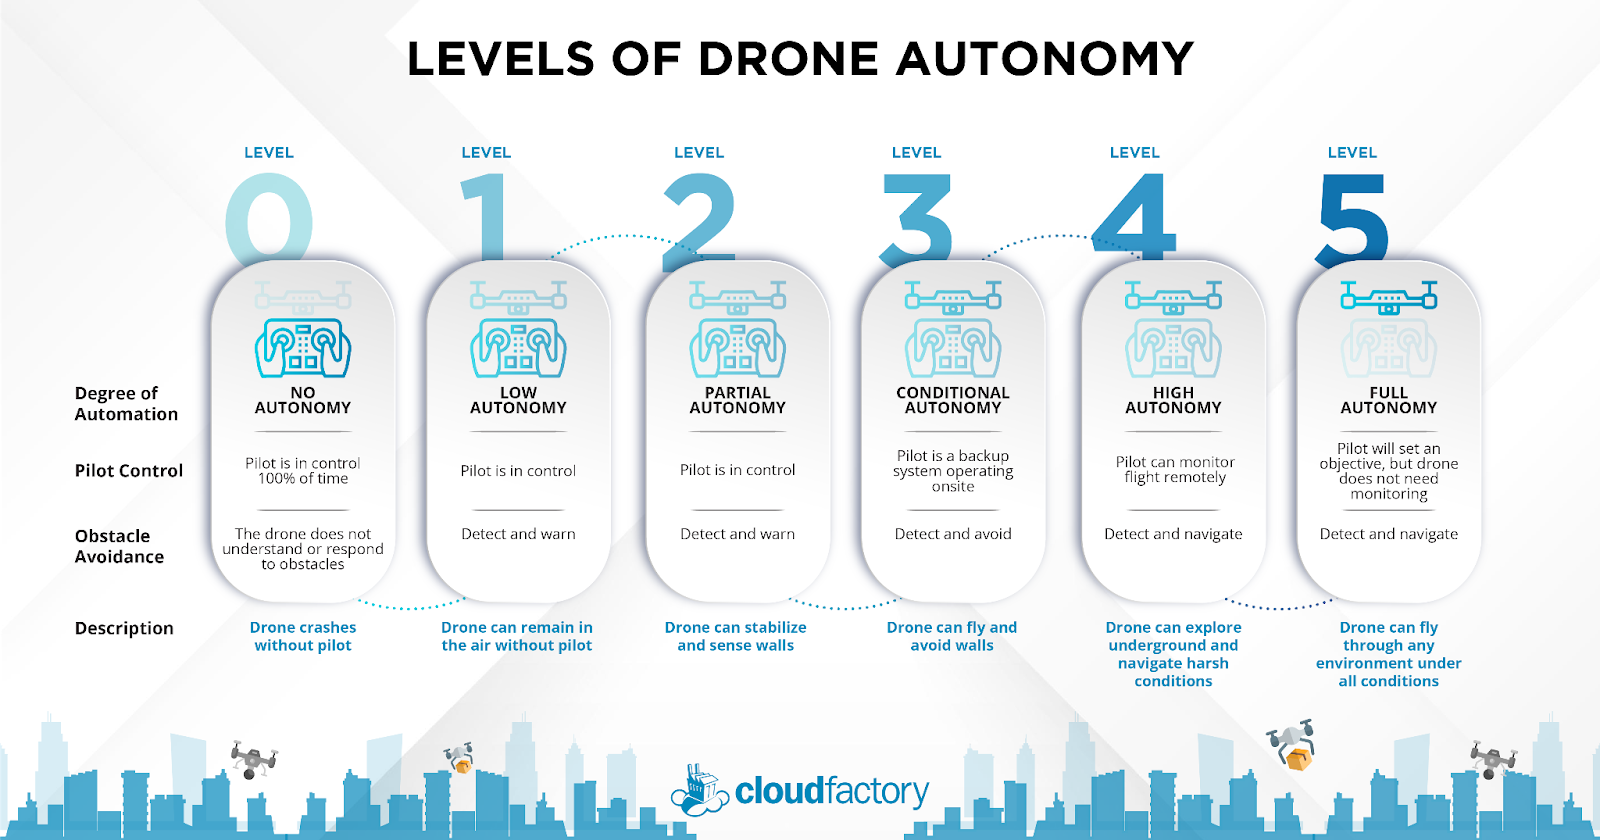
\includegraphics[width=0.7\linewidth]{images/drone_autonomy_levels.png}
	\caption[Einteilung Automationsklassen von \gls{uav}]{Einteilung Automationsklassen von \gls{uav}: Vom niedrigsten Level (0) zum höchsten Level (5) steigt der Automationsgrad, von \cite{cloudfactoryBreakingLevelsDrone}).}
	\label{fig:automation_levels}
	\end{figure}

Das \gls{lba} erlässt zudem Regelungen, wonach ein autonomer Flug \enquote*{[...] derzeit nicht zulässig [ist]; Fernpiloten müssen jederzeit eingreifen können. [...]}\cite{openuavadminDatenverbindungUndFlugmodi}.  

Der bisherige Stand des Projektes steht im Übergang von Automationsklasse 3 auf Klasse 4. Allerdings fehlen generalisierte Anwendungsfälle (später gezeigt) sodass die Drohne noch nicht wie gewünscht, Hindernissen ausweicht (das bisherige Verhalten beschränkt sich auf sicheres Landen beim Erkennen von Hindernissen).

%
%\begin{figure}[!h]
%	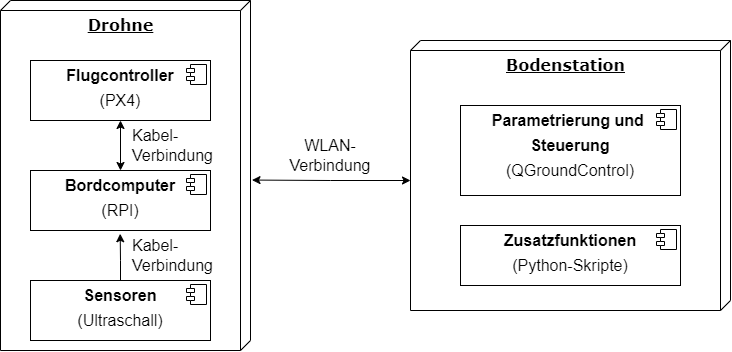
\includegraphics[width=\linewidth]{images/setup_initial_simple.drawio.png}
%	\caption{Gesamtbild Zusammenwirken der Bauteile der Drohne}
%	\label{fig:setup_initial}
%	\end{figure}
%
%
%Die Verwendung von \gls{ros} \cite[Kapitel 3.6.1]{wirthErweiterungBestehendenDrohne2022} als treibende Software zur Automatisierung ist bisher weder ausreichend entwickelt noch empfohlen \cite{haraldwirthNachfolgerInfoStudienarbeitAutonome2022}, aber doch notwendig für eine erfolgreiche Umsetzung des Projektes \cite[Kapitel 9.1]{wirthErweiterungBestehendenDrohne2022a}.
%Außerdem soll zur Automatisierung auf dem \gls{rpi} das Framework \gls{ros} verwendet werden, wie in \cref{chap:ros} zum Einsatz.

Wie in \cref{chap:sota} erläutert, wird die Modelldrohne Holybro S500 verwendet. Um diese Fliegen zu dürfen, bestehen in Deutschland mehrere Vorraussetzungen\footnote{\url{https://lba-openuav.de/onlinekurs/lehrmaterial}}:
\begin{compactitem}
	\item Drohnenführerschein: Unterkategorie A2 (\gls{uas} bis $4kg$, $5m$ Abstand zu Menschen, kein Überfliegen von Menschenansammlungen, nur auf Sichtweite fliegen)
	\item Höhenmesser: die maximale Flughöhe von $120m$ darf nicht überschritten werden
	\item Fernidentifizierung: Pflicht zum Mitführen eines ADS-B Transmitters\footnote{\url{https://de.wikipedia.org/wiki/Automatic_Dependent_Surveillance}} 
	\item Haftpflichtversicherung: Pflicht zum Versichern und Kennzeichnen der Drohne
	\item \enquote{Filmen, fotografieren oder das Anfertigen von Tonaufnahmen ist verboten, wenn: [...] die Aufnahmen für Gesichtserkennung oder andere automatisierte Prozesse verwendet werden}
\end{compactitem}

Somit der Einsatz der Drohne im öffentlichen Raum streng untersagt. Tests beschränken sich auf Flüge nahe am Boden, fernab der Zivilisation.

\section{Peripherie an der Drohne}
Im Flugcontroller integriert sind mehrere Sensoren (Beschleunigung, Gyroskop, Magnetometer, Barometer). Neben diesen besitzt das Modell einen dedizierten \gls{gps}-Empfänger. Nachfolgend ist dargestellt, wie diese Sensoren ausgewertet werden können.

%\subsection{Kommunikation mit dem Flugcontroller}\label{chap:drone_coms} Der Flugcontroller kann als eigenständige Einheit betrieben werden. Dabei kann die Drohne mittels Fernsteuerung gesteuert werden. In diesem manuellen Betrieb ist die Drohne nicht programmierbar.\newline Für zusätliche Funktionen stellt der Flugcontroller einen USB-Port und mehrere Telemetry-Ports bereit. Alle Daten zu und vom Flugcontroller werden mit dem \gls{mav}\footnote{\url{https://mavlink.io/en/}}-Protokoll übertragen. Die Daten können von Bodenstation oder entsprechenden Anwendungen ausgewertet werden. Mit der USB-Verbindung kann eine direkte Verbindung zu einem PC hergestellt werden. Somit lässt sich die Drohne einrichten, allerdings muss die Kabelverbindung zum Flug getrennt werden. Auch wird zur allgemeinen Flugsteuerung davon abgeraten die USB-Schnittstelle zu verwenden, da es bei der Datenübertragung zu Verzögerungen kommen kann.\newline Der auf die Drohne montierte \gls{rpi} kommuniziert mit dem Flugcontroller über den Telemetry-Port. Hierbei wird eine UART-Verbindung (bidirektionale Kommunikation über je eine Signalleitung) verwendet, da diese im Gegensatz zu USB einfacher zu programmieren ist und verzögerungsfrei arbeitet.\newline Das \gls{mav}-Protokoll zeichnet sich durch eine allgemein hohe Effizienz (geringer Overhead) aus. Nachrichten werden nach Themengebieten (z.B. Nachrichten vom Typ \textit{HIGHRES\_IMU} liefern Sensordaten) geordnet. Somit lässt sich eine bestimmte Eigenschaft von Interesse auslesen bzw. einspeisen. Um verlässliche Resultate beim Übertragen der Daten zu erhalten, enthalten so gut wie alle Nachrichten den Zeitpunkt des Absendens.\newline Der Flugcontroller kann konfiguriert werden nur Nachrichten bestimmter Typen zu versenden, um die Rechenlast zu verringern und höhere Übertragungsraten zu erlauben. Zu den möglichen Einstellungen zählen bspw. \textit{Normal} (Verbindung zu Bodenstation) oder \textit{Onboard} (Verbinfung zu mitgeführtem Computer) wobei ca. 40 respektive 50 Nachrichtentypen versendet werden. Wird die Einstellung \textit{Normal} verwendet, so werden keine Nachrichten vom Typ \textit{HIGHRES\_IMU} versendet. Außerdem wird für jeden Nachrichtentyp die Frequenz festgelegt, sie beträgt bspw. für die \textit{HIGHRES\_IMU} $50Hz$. 

%\subsection{Sensoren des Flugcontrollers} Ausgelesen vom Flugcontroller werden die Sensoren der \textit{HIGHRES\_IMU}. Dabei werden Messpunkte mit hoher Frequenz und Auflösung bereitgestellt. Eine Verarbeitung muss die Daten filtern um weitere Berechnungen durchführen zu können. Zur Verwendung kommt \gls{ros}, 

\subsection{Navigation mittels GPS}
Die Navigation der Drohne erfolgt vorrangig über \gls{gps}. Mit solchem System können die aktuelle Position und Geschwindigkeit festgestellt werden. Für ein reales System muss ein eventueller Ausfall der \gls{gps}-basiertern Navigation in Betracht gezogen werden, denn \gls{gps} setzt klare Sicht zum Himmel und eine Verbindung zu mindestens 4 Satelliten voraus. [Quelle]

Fällt das \gls{gps} aus, ist die Drohne jedoch noch nicht völlig blind. Beschleunigungssensor, Gyroskope und Kompass bilden eine \gls{imu}, mit deren Daten mittels eines \textit{Extended Kalman Filter} die ungefähre Position berechnet werden kann. Das Ergebnis kann durch das Überlagern der Messwerte mehrerer Sensoren verbessert werden, bspw. indem sich an einem Kamerabild mit den bereits bekannten Abständen zu Objekten orientiert wird. 
%Der Flug der Drohne kann trotzdem zu jeder Zeit von Umwelteinflüssen (bspw. Wind) beeinflusst werden. Dabei kann sich die Position trotzdem unbemerkt verändern.

Ein weiteres Problem ist die totale Abhängigkeit von \gls{gps} in Bezug auf Zielfindung. Selbst wenn die Drohne direkt über dem Zielpunkt fliegt, aber \gls{gps} ausfällt, kann sie keine Erfolg verzeichnen. Für die Flugplanung wäre folglich ein zweiter Sensor von notwendig, der ohne \gls{gps} zum Zielpunkt navigieren kann. Für das Aufwinden des Zieles stehen mehrere Technologien zur Verfügung:
\begin{compactdesc}
    \item[Ortung] eines Sender (Ultraschall oder Infrarot) welcher durchgängig Signale sendet. Die Drohne bewegt sich dann immer auf den Sender zu.
    \item[Erkennung] einer Struktur oder Bildes (Marker) mittels Kamera.
\end{compactdesc}
%
%\subsection{Routenplanung}
%Weiterhin kann mit \gls{gps} und dem vorher eingeführten Magneten-Prinzip (siehe \cref{chap:sota}) kein Erfolg bei der Navigation erzielt werden, falls das Ziel nicht auf direktem Weg erreichbar ist. [noch ein Bild] Die Konsequenz ist, dass ein autonomer Flug eine Umgebungskarte und Routenplanung benötigt.
%Dazu muss die Drohne muss ihre Umgebung per Sensor wahrnehmen und ein 3D-Modell der Umgebung erstellen. Dazu werden weitere Sensoren und ein Wegfindungs-Algorithmus benötigt.
%
%Eine verfügbare Routenplanung soll den optimalen Weg von einem gegeben Start zum Ziel finden.
%Für die Drohne, die sich auf beliebigem Weg durch die Luft bewegen kann, ist die Luftlinie eine erste und sehr gute Näherung hierfür.
%Um den optimalen Weg zu finden, muss der Ansatz verschiedene Faktoren auf dem Weg berücksichtigen. Es ergeben sich wirksame Beispiele:
%\begin{compactdesc}
%	\item[Hindernisse:] Ein Berg mit Tunnel versperrt den Weg. Sollte die Drohne den Tunnel bemerkt haben, sollte sie hinein fliegen oder um den Berg herum?
%	\item[Luftwiderstand:] Gegenwind bremst die Drohne stark ab. Sollte sich die Drohne näher am Boden/ weiter in der Luft aufhalten, um dem Wind zu entgehen? 
%\end{compactdesc}
%Das Beispiel des Luftwiderstands erscheint komplex und erfordert spezielle Sensoren zur Messung. Deshalb kann es in dieser Arbeit nicht näher betrachtet werden.
%Eine gezielte Umgehung von Hindernissen sollte allerdings Teil des autonomen Fluges sein.
%

\subsection{Hinderniserkennung durch Ultraschallsensoren}\label{chap:ultrasonic}
Mit einem Ultraschallsensor kann der Abstand zu Objekten gemessen werden. 

Das Prinzip der Ultraschallortung besteht aus 3 Schritten:
\begin{compactenum}
	\item Aussenden des Messimpulses. Daraufhin generiert der Sensor Ultraschall-Impulse.
	\item Empfangen der Messimpulse. Der Sensor setzt ein Signal wenn ein Echo empfangen wird.
	\item Auswerten der Signallaufzeit. Die Impulse bewegen sich mit Schallgeschwindigkeit im Medium zum Messobjekt und zurück.
\end{compactenum}

Verwendet werden Ultraschallsensoren an der Drohne, welche Messimpulse in die Umgebung aussenden. Für eine exakte Auswertung der Signallaufzeit müssten Umgebungstemperatur, Luftdruck und Luftfeuchte bekannt sein. Den größten Einfluss spielt dabei die Temperatur. Druck und Feuchte wirken nur mit jeweils maximal auf das Ergebnis ein 5\% bzw. 2\%.\newline
Die Formel zur Bestimmtung der Entfernung eines Objektes lautet ist gegeben in Formel \ref{mat:dist_by_t}. Benötigt wird die Schallgeschwindigkeit $c_{20}$ bei $20$\textcelsius und der Temperaturkoeffizient $\alpha_{20}$\cite[Seite 152]{grudenSensorikUndMesswertverarbeitung2022}.
\begin{align}
	s &=\frac{1}{2}c\cdot t\\
	&=\frac{1}{2}c_{20}(1+\alpha_{20}(\vartheta-20\textrm{\textcelsius})) t	\label{mat:dist_by_t}
\end{align}

\section{Bilderkennung und Obstacle Avoidance}
Mannigfaltige Prinzipien fallen in den Bereich der Bilderkennung. Der Fokus dieses Projektes, das Erkennen und Ausweichen von Hindernissen wird \enquote{Obstacle Avoidance} genannt. Es ist nicht zu verwechseln mit \enquote{Obstacle Detection}, dem Erkennen und Klassifizieren von Bildinhalten. Nachfolgend vorgestellt werden Techniken die hier zum Einsatz kommen könnten. 
\paragraph*{SLAM Algorithmus}\label{chap:slam}
\Gls{slam} Techniken entstanden bereits in den 1980-1990 Jahren und wird bspw. bei Robotern eingesetzt, die in Hallen navigieren (kein \gls{gps} verfügbar). Dazu kommen mit Kamerasysteme in Verbindung mit Entfernungssensor (Sonar, Radar, Lidar) zur Verwendung . Die Ergebnisse von \gls{slam} können nicht garantiert werden und sind nicht reproduzierbar, weshalb es in keinen kritischen Umgebungen (bspw. wenn Verletzungsrisiko besteht) eingesetzt werden kann.

Allgemein wird \gls{slam} durch einen modularen Prozess beschrieben: \begin{compactdesc}
    \item[Lokalisierung:] per Motorfortschritt, \gls{imu}, Kamera, etc.\newline
    Bei v\gls{slam} kommen folgende Prinzipien zum Einsatz:
\end{compactdesc}
\begin{compactitem}
    \item Markov-Lokalisierung: Wahrscheinlichkeit des Aufenthaltsortes wird angenommen und über Zeit verfeinert. Iterativ, Ressourcenaufwendig.
	\item Kalman-Filter: Ermöglicht basierend auf Sensordaten schnelles wiederfinden aktueller Position. Anfällig bei Verlust von Kamerabildern
	\item Monte-Carlo-Lokalisierung: auch Partikelfilter genannt, nimmt Wahrscheinlichkeiten für jeden Ort an. Genauer als Markov, lineare Komplexität. Weniger Speicher als Kalman. Nachteil: Stillstand ohne sich ändernde Sensordaten
\end{compactitem}
\begin{compactdesc}
    \item[Messung:] per Reichweite, Marker in Umgebung
\end{compactdesc}
%was sollte hier noch hin

\paragraph*{Visual SLAM} 
Eine Sonderform des \gls{slam} ist Visual \gls{slam} (vSLAM). Bei diesem werden ausschließlich Kameras zur Erkennung der Umgebung eingesetzt. Der Algorithmus verwendet zusätzliche Sensordaten um die Bewegung der Kamera in die Berechnung der Position einzubeziehen.

\paragraph*{Stereokamera}\label{chap:stereovision}
Verwendet mehrere Kameras aus parallelverschobenen Bildern Tiefeninformationen zu gewinnen. also Abstand zu Punkten im Bild zu erkennen.
\paragraph*{Optical Flow}
Auswertung der Bewegung von Objekten in Videoabläufen. Kann schlecht zwischen Bewegung der Kamera und Bewegung der Objekte unterscheiden. Ungenau, da Kameras immer eine Verzerrung besitzen. 

\section{Robot Operating System}
koennte auch mal noch... ist erklaert in \cite[Kapitel 2.2]{wirthErweiterungBestehendenDrohne2022a}
\chapter{Stand der Technik}
In diesem Kapitel werden die Grundlagen verwendeter Software erläutert.
\section{Erweiterte Flugmodi der Drohne}\label{chap:intro_capabilities}
Bei Verwendung der Drohne in Verbindung mit einer Bodenstation, wird die aktuelle Position auf einer Karte eingezeichnet. Von diesem Punkt aus kann der Drohne eine Wegvorgabe eingespielt werden, der \enquote{Mission-Mode}. Dabei enthält die Karte Informationen zur ungefähren Beschaffenheit der Umgebung, sodass die Drohne nicht Tiefer fliegen würde als der Boden der Karte. Gleichzeitig sind die standardmäßigen Sicherheitsmaßnahmen eingestellt, bspw. eine Mindesflughöhe von $4m$ einzuhalten. Neben der Wegvorgabe können dem Flugcontroller weiterhin verbotene Zonen mitgeteilt werden, die nicht durchflogen werden dürfen, genannt \textit{\enquote{Geo-Fence}}. Der Algorithmus sieht derartige Zonen als Hindernis an. Bei Kontakt mit ihnen wird ein Failsafe ausgelöst. \textit{PX4} kennt zwei derartige Modi:
\begin{description}
    \item[Failsafe GeoFence:] Ein Zylinder dessen Durchmesser von der Funkreichweite der Fernbedienung und maximaler Flughöhe beschränkt ist. Bei Durchbruch verfällt die Drohne standardmäßig in den \enquote{Return-Mode} und kehrt zu ihrer Ausgangsposition zurück.
    \item[GeoFence Plan:] Kreise oder Polygone auf Karte die nicht durchflogen oder verlassen werden dürfen (je nach Einstellung). Bei Bruch der Bedingung verfällt die Drohne in den \enquote{Hold-Mode} und bleibt schlicht stehen.
\end{description}

Es ist also bereits mit Bordmitteln möglich das Flugverhalten zu beeinflussen. Für das Vorgehen mit \textit{Avoidance} kommt der \enquote{Offboard-Mode} zum Einsatz. In diesem Modus werden dem Flugcontroller ständig neue Anweisungen, als nächster Wegpunkt, eingespeist.

Weiterhin können der Drohne im Missionsmodus sogennante \gls{roi} mitgeteilt werden. Ist eine Kamera an der Drohne vorhanden, wird diese gezielt auf die Positionen gerichtet. Ist keine Kamera explizit definiert richtet sich die Drohne mit dem Bug in Richtung der \gls{roi} aus. Da die Drohne sowohl vorwärts als auch seitwärts fliegen kann, hält sie durchgehend auf den Punkt zu.

\section{ROS und Avoidance}
Das Projekt \enquote{Obstacle Detection and Avoidance}\cite{dronecodestiftungObstacleDetectionAvoidance2023}, auf GitHub verfügbar als PX4-Avoidance\footnote{\label{note1}\url{https://github.com/PX4/PX4-Avoidance}}, hier nur \textit{Avoidance} genannt, entstand in enger Zusammenarbeit mit der Dronecode Stiftung an der ETH Zürich, dem Ursprungsort aller \textit{PX4}-Software. Es arbeitet innerhalb einer \acrshort{ros}-Umgebung.

Es stehen im Projekt 3 Algorithmen zur Verfügung, die unabhängig voneinander zu betrachten sind. Alle dienen der Anpassung der Flugbahn in unbekannter Umgebung:
\begin{description}
    \item[Local Planner:] Navigiert um Hindernisse in der direkten Umgebung
    \item[Global Planner:] Speichert nahezu vollständige Karte der Umgebung und erlaubt Navigation durch Labyrinth-artige Umgebung
    \item[Safe Landing Planner:]
\end{description}

Die Software von \textit{Avoidance} erhält die Daten des Flugcontrollers über das Zwischenprogramm \textit{mavros} (\acrshort{mav}-zu-\acrshort{ros}-Übersetzung, siehe \cite[Kapitel 5.2/5.4]{markusreinErweiterungBestehenderDrohnen2023}). Es sind die Soll-Trajektorie und Sensordaten vom Flugcontroller bekannt. Außerdem wird zur Navigation eine \textit{Punktwolke} (siehe \cref*{chap:intro_pointcloud}) der Umgebung eingespeist. Falls das Programm ein Hindernis in der Flugbahn erkennt, wird eine angepasste Trajektorie an den Flugcontroller ausgegeben.

Die Software kann nicht direkt auf dem Flugcontroller ausgeführt werden, da die Berechnungen sehr viele Ressourcen (Rechenkapazität, Speicher) benötigen. Weiterhin empfehlen die Entwickler, zuerst den Local Planner zu implementieren, da dieser am besten funktioniert. Offizielle Empfehlungen der Entwickler verwenden leisstungsstarke Hardware wie Nvidia Jetson (Hardware-Unterstützung für Bildverarbeitung) oder Intel RealSense (Kamera mit Tiefenerkennung).

Im Zusammenhang mit der Software sind letztere bereits erprobt. Aufgrund des hohen Preises können sie nicht in diesem Projekt verwendet werden, siehe \cite[Kapitel 4.3.8]{wirthErweiterungBestehendenDrohne2022}. Als Alternative können auch Stereokameras verwendet werden. Beispielcode zur Einbindung von Tiefenbildern ist unter Github (siehe \cref{note1}) vorhanden. 

%Stereokamera liefert genaue Karte der Umgebung, ähnlich einem Lidar.
%Andere Methoden arbeiten eventuell nicht mit Avoidance zusammen. Doch doch

\section{Hinderniserkennung und ROS Punktwolken}\label{chap:intro_pointcloud}
Als Verschiedene Prinzipien stehen zur Hinderniserkennung zur Verfügung. Als Eingabegröße für \textit{Avoidance} müssen die verarbeiteten Bilder im Punktwolkenformat als \acrshort{ros}-Topic vorliegen.
%Quellen nicht eindeutig
%Der Fokus dieses Projektes, das Erkennen und Ausweichen von Hindernissen wird \enquote{Obstacle Avoidance} genannt. Es ist nicht zu verwechseln mit \enquote{Obstacle Detection}, dem Erkennen und Klassifizieren von Bildinhalten.
Nachfolgend vorgestellt werden die grundlegenden Techniken der Bilderkennung. 
\subsection{SLAM Algorithmus}\label{chap:slam}
\Gls{slam} Techniken entstanden bereits in den 1980-1990 Jahren und werden bspw. bei Robotern eingesetzt, die in Hallen navigieren (für die kein \acrshort{gps} verfügbar ist). Zum Einsatz kommen Kamerasysteme in Verbindung mit Entfernungssensoren (Sonar, Radar, Lidar). Die Ergebnisse von \gls{slam} können nicht garantiert werden und sind nicht reproduzierbar, weshalb es in keinen kritischen Umgebungen (bspw. wenn Verletzungsrisiko besteht) eingesetzt werden kann.

Allgemein wird \gls{slam} durch einen modularen Prozess beschrieben:
\begin{description}
    \item[Lokalisierung:] per Motorfortschritt, \gls{imu}, Kamera, etc.%\newline Bei v\gls{slam} kommen folgende Prinzipien zum Einsatz:
    \item[Kartengenerierung:] durch einen der Algorithmen
\begin{itemize}
    \item Markov-Lokalisierung: Wahrscheinlichkeit des Aufenthaltsortes wird angenommen und über Zeit verfeinert; Iterativ; Ressourcenaufwendig
	\item Kalman-Filter: Ermöglicht basierend auf Sensordaten schnelles wiederfinden aktueller Position; anfällig bei Verlust von Eingangsdaten
	\item Monte-Carlo-Lokalisierung (Partikelfilter): nimmt Wahrscheinlichkeiten für jeden Ort an; genauer als Markov-Filter; lineare Komplexität; Weniger Speicher als Kalman-Filter; Nachteil: Stillstand ohne sich ändernde Sensordaten
\end{itemize}
    \item[Messung:] per Reichweite, Marker in Umgebung
\end{description}
%was sollte hier noch hin

\paragraph*{Visual SLAM,}kurz vSLAM, stellt eine Unterform des \gls{slam} dar, bei der ausschließlich Kameras zur Erfassung der Umgebung eingesetzt werden. Algorithmen verwenden zumeist zusätzlich die Daten der \acrshort{imu}, um die Bewegung der Kamera in die Berechnung der Position einzubeziehen.

\subsection{Stereokamera}\label{chap:stereovision}
Verwendet mehrere Kameras aus parallelverschobenen Bildern Tiefeninformationen zu gewinnen. also Abstand zu Punkten im Bild zu erkennen.
\subsection{Optical Flow}
In Bewegungsabläufen werden Objekten verfolgt und können somit relativ zur Kamera bestimmt werden. Das Prinzip wird auch von Lebewesen im Gehirn angewandt. Dabei kann schlecht zwischen der Bewegung der Kamera und der Bewegung von Objekten unterschieden werden. Ungenau, da Kameras immer eine Verzerrung besitzen. 

\subsection{Punktwolkenformat}
Die Möglichkeiten Optical Flow und Stereokamera erzeugen jeweils Tiefenkarten. In diesen Bildern sind, zumeist als Graustufen, Pixel je nach Entfernung zur Kamera gekennzeichnet. Zur Umwandlung als Punktwolke muss jedes Pixel abgetastet werden um als Koordinate im 3D-Raum dargestellt werden zu können. Das \acrshort{ros} beinhaltet sowohl Progamme zur Stereoverarbeitung basierend auf OpenGL\footnote{siehe \url{http://wiki.ros.org/stereo_image_proc}}, als auch die Erzeugung von Punktwolken\footnote{siehe \url{http://wiki.ros.org/depth_image_proc}}.

\chapter{Aufarbeitung bestehendes Drohnenprojekt}
\label{chap:main}
% !TeX spellcheck = de_DE
In diesem Kapitel wird das bestehende Projekt aus nachvollzogen und überarbeitet. Inhalte sind das Testen bestehender Vorlagen aus \cite{wirthErweiterungBestehendenDrohne2022} und \cite{wirthErweiterungBestehendenDrohne2022a}, sowie das Aufsetzen einer neuen Arbeitsumgebung wie in beschrieben in \cite{haraldwirthNachfolgerInfoStudienarbeitAutonome2022}, siehe \cref{chap:nachfolger}.

\section{Inbetriebnahme}
Zur Aufarbeitung des Projektes steht ist die Drohne bestehend aus Rahmen, Flugcontroller, Motoren mit Propellern, Ultraschallsensoren und Akku bereit. Nicht vorhanden sind die RC-Fernsteuerung und der auf die Drohne montierte \gls{rpi}. Ursprünglich verwedet wurde ein \gls{rpi} 4 Model B mit $2GB$ \gls{ram} als Bordcomputer, der mit dem Flugcontroller kommuniziert, dessen Daten über ein Netzwerk verbreitet und auch Anweisungen zum Flug geben kann. Gleiches kann auch mit dem \gls{rpi} 3 Model B+ bewerkstelligt werden. Dieser bestitzt im Gegensatz nur 1GB \gls{ram} und weniger Rechenleistung.
Die gelieferte SD-Karte enthält das Betriebssystem Raspbian OS in der Ausführung als 32-bit Betriebssystem. Sowohl \gls{rpi} Model 4 als auch Model 3 besitzen zwar 64-bit Prozessoren, allerdings wird bei bis zu 4GB \gls{ram} das 32-bit Betriebssystem empfohlen um diesen effektiver auszunutzen.
Der verwendete \gls{rpi} startet somit problemlos.
Beim Systemstart wird automatisch der WLAN-Hotspot aktiviert und der MAVLINK-Server (mavlink-routerd) gestartet. %und verschiedene Docker Container
%Auf dem \gls{rpi} 3 führt dies führt zu einer hohen Systemauslastung, 1 von 4 CPU-Kernen ist permanent zu 100% belegt. Auch die Temperatur erhöht wodurch sich die Kerntemperatur auf ca 53°C erhöht. --- anscheinend doch nicht

\subsubsection{Verbindung Flugcontroller mit \gls{rpi}}
Durch das automatische Setup des \gls{rpi} sollte die Drohne mit dem Einstecken des Stromes bereit zum Flug sein. In \cite[Kapitel 4.3.6]{wirthErweiterungBestehendenDrohne2022} ist der erste Schritt beschrieben als "Test der Verbindung". Der \gls{rpi} wird mit dem Flugcontroller  per Serieller Schnittstelle verbunden (siehe auch \cref{chap:drone_coms}). Dazu wurde eigens ein Kabel entwickelt, welches die UART-Pins des \gls{rpi} mit dem TELEM2-Port des Flugcontrollers verbindet. Es ist zu beachten, dass keine Dokumentation bezüglich der Belegung der Kabeladern (per Jumper an den \gls{rpi} zu Stecken) gegeben ist. Ein Ausmessen des Kabels ergab:
\begin{compactitem}
    \item Schwarz: Masse -> Pin 06 des \gls{rpi}
    \item Braun: UART-Receive (Rx) des Flugcontrollers -> Pin 08 (Tx) des \gls{rpi}
    \item Weiß: UART-Transmit (Tx) des Flugcontrollers -> Pin 10 (Rx) des \gls{rpi}
\end{compactitem}
Anschließend soll die Verbindung wie in \cite[Kapitel 4.3.6]{wirthErweiterungBestehendenDrohne2022} beschrieben, die MAVLINK-Konsole geöffnet werden. Jedoch ist das Programm \textit{mavproxy} auf dem aktuellen Image nicht vorhanden. Um das weitere Vorgehen zu konkretisieren wurde das Programm nachinstalliert\footnote{\url{https://ardupilot.org/mavproxy/docs/getting_started/download_and_installation.html\#mavproxy-downloadinstalllinux}}. Das Starten des Konsolenprogrammes ist nur möglich, wenn der MAVLINK-Server (Prozess \textit{mavlink-routerd}) nicht läuft (ansonsten ist die Serielle Schnittstelle blockiert). Mit dem Befehl: 
\texttt{mavproxy.py -{}-master=/dev/serial0 -{}-baudrate=921600}
kann schließlich die Kommunikation des \gls{rpi} mit der Drohne verifiziert werden.

Für das weitere Vorgehen wird das allzeit vorliegende Programm \textit{mavlink-routerd} verwendet. Es arbeitet als Server im Hintergrund und verbreitet MAVLINK-Nachrichten im Netzwerk. Auch \textit{mavproxy} stellt solch eine Funktionalität bereit, allerdings wird aufgrund von zu erwartenden Leistungseinbußen davon abgeraten\footnote{\url{https://ardupilot.org/mavproxy/docs/getting_started/forwarding.html}}. Die Konfiguration des \textit{mavlink-routerd} wird wie in \ref{fig:mav_controller} dargestellt angepasst. Dadurch kann sich jedes Netzwerkgerät (auch der \gls{rpi} selbst) über das \gls{udp}-Protokoll mit dem Flugcontroller verbinden. Auch kann ein PC/ Smartphone eine Verbindung zum Flugcontroller über das Netzwerk herstellen. Mit der neuen Konfiguration steht sowohl ein TCP-Server, als auch ein UDP-Server zur Verfügung. Eine Auswertung zur Verwendung des geeignetsten Protokolls folgt in \cref{chap:bench_tcp_udp}. In Bild \ref{fig:mavconf_mavproxy} ist das Vorgehen zur Verbindung über einen Netzwerkknoten und das erneute Ausführen des Funktionstests dargestellt.

\begin{figure}
  \centering
    \subfloat[Alte Konfiguration von \texttt{mavlink-routerd}]{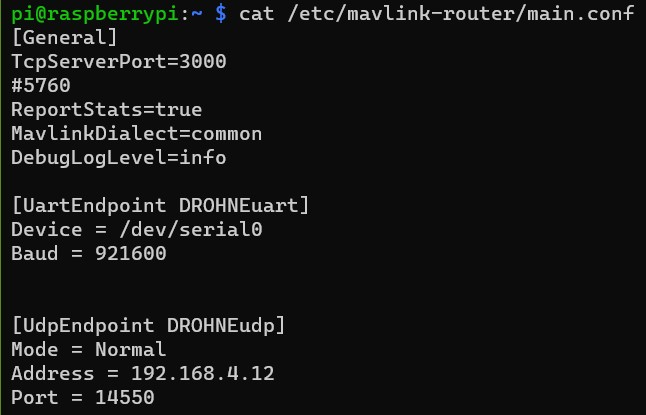
\includegraphics[width=0.5\textwidth]{images/mavlink.conf.old.jpg} \label{fig:mavconf_old}}
    \subfloat[BILD FALSCH, das ganze funktioniert anders! Neue Konfiguration von \texttt{mavlink-routerd}]{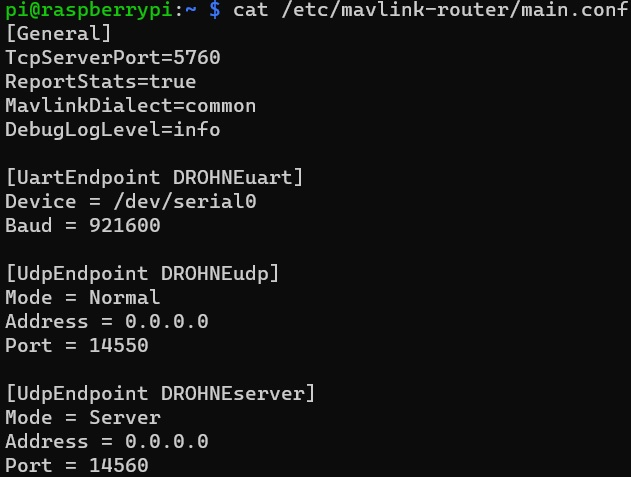
\includegraphics[width=0.5\textwidth]{images/mavlink.conf.new.jpg} \label{fig:mavconf_new}}
    
	\subfloat[Verbindung mittels \texttt{mavproxy} auf dem \gls{rpi}]{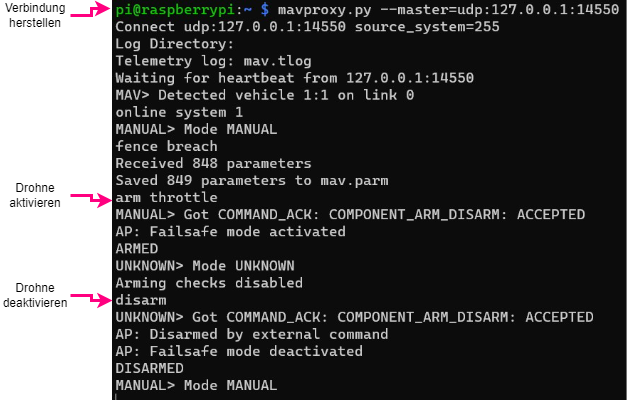
\includegraphics[width=0.8\textwidth]{images/mavlink_connect.png} \label{fig:mavconf_mavproxy}}
    
	\caption{Konfiguration und Verwendung von \texttt{mavlink-routerd}}
\label{fig:mav_controller}
\end{figure}

\subsubsection{Verbindung Flugcontroller mit PC}
Als \gls{gcs} zur Kommunikation mit dem Flugcontroller wird das Programm QGroundControl, wie in \cite[Kapitel 3.4]{wirthErweiterungBestehendenDrohne2022} vorgeschlagen, verwendet. Mit diesem können beliebige Drohnen konfiguriert, parametriert und geflogen werden. Der Flugcontroller kann dazu per Micro-USB mit dem PC verbunden werden und das Programm findet selbigen automatisch.

Per Knopfdruck kann hier die Funktion \textit{arm} ausgeführt werden und die Propeller beginnen zu Drehen. Das Programm stellt sogleich fest, dass keine Fernsteuerung verbunden ist und verfällt in den \textit{manuellen Modus}. Nach einigen Sekunden wird die Drohne automatisch wieder \textit{disarmed} und die Propeller gestoppt um Schäden zu vermeiden.

Um den Flugcontroller über das drahtlose Netzwerk des \gls{rpi} anzusteuern, muss das Programm QGroundControl manuell konfiguriert werden. Dazu muss eine Einstellung unter \textit{Comm Links} vorgemerkt werden, in welcher die IP-Adresse des \gls{rpi} und der \textit{TcpServerPort} des MAVLINK-Servers (siehe Bild \ref{fig:mavconf_new}) eingepflegt werden.

Mithilfe des Programmes QGroundControl kann eine Drohne weiterhin ohne RC-Fernsteuerung geflogen werden. Es stehen Werkzeuge zur Planung eines \enquote{autonomen Fluges} bereit\footnote{\url{https://docs.qgroundcontrol.com/master/en/PlanView/PlanView.html}}. Dazu lassen sich GPS-Wegpunkte auf einer Karte anlegen, die die Drohne später selbstständig abfliegt. Außerdem stellt QGroundControl Funktionen zur Verfügung, eine Drohne mittels Joystick (virtuell oder per angeschlossenem Konsolen-Controller) zu steuern\footnote{\url{https://docs.px4.io/main/en/config/joystick.html}}.

\subsubsection{Benchmark zur Verbindung von PC zum Flugcontroller}\label{chap:bench_tcp_udp}
Zur Durchführung des Projektes steht keine physikalische RC-Fernsteuerung zur Verfügung, sondern es können nur Wegpunkte gesetzt oder ein Konsolen-Controller am PC verwendet werden. Für letzteren Fall ist es entscheident, dass die Daten über das mavlink-Protokoll zum Flugcontroller gesendet werden. Dabei ist die Verbindung über das Netzwerk des \gls{rpi} langsamer als die Verwendung einer echten Fernsteuerung. Um trotzdem die optimale Reaktionsfähigkeit zu erreichen, soll verglichen werden, ob die Verbindung über TCP-Protokoll oder UDP-Protokoll schneller ist\footnote{\url{https://stackoverflow.com/questions/47903/udp-vs-tcp-how-much-faster-is-it}}. Die entscheidenden Kriterien sind:
\begin{compactitem}
    \item Latenz: Reaktionsfähigkeit des Flugcontrollers
    \item Bandbreite: Auslastung des Datenkanals 
\end{compactitem}

[TODO]

\subsection{Einbindung von Funktionalität mittels Docker-Containern}
Weitere Funktionen der Drohne sollen mit \gls{ros} bereitgestellt werden. Da dieses nicht auf dem Betriebssystem des \gls{rpi} lauffähig ist, wird es als Docker Containern bereitgestellt.

Aufbauend auf den Projekten \cite{wirthErweiterungBestehendenDrohne2022}, \cite{wirthErweiterungBestehendenDrohne2022a} sollen bestehende Docker-Container wiederverwendet werden. Eine erste Inspektion mit \texttt{docker images} zeigt, dass lediglich das \texttt{hello-world} Beispiel bereits heruntergeladen wurde und im Programmspeicher bereit liegt. Weiterhin zeigt der Befehl \texttt{docker ps -a} dass auch nur dieses Beispiel bisher ausgeführt wurde. Im bestehenden Quellcode enthalten sind verschiedene Tests. Schon der Test 1 importiert einen Container aus \enquote{arm64v8/ros:galactic}. Das besagte Abbild ist für eine 64-bit ARM Architektur gedacht und damit auf dem gelieferten Betriebssystem nicht lauffähig. In weiteren Tests 3 und 4 wurde dieser Mangel erkannt und versucht zu korrigieren.

\paragraph*{Test 1} dient der Demonstration von ROS im Zusammenspiel mit Docker und wird in dieser Arbeit nicht betrachtet, da er keine erkennbare Funktion erfüllt.

\paragraph*{Test 3} betrachtet das Zusammenwirken mehrer Container über Netzwerkenpunkte. Das Sende- und Empfangsverhalten wurde untersucht um möglichst effizienten Datenaustausch bereitzustellen. Der Test soll mit dem Befehl \texttt{docker-compose up} gestartet werden. Zum Zeitpunkt der Ausarbeitung dieser Arbeit schlägt dies erst einmal fehl, denn das vorgesehene Ubuntu Image für den Server (\enquote{ubuntu:impish}, zu finden in Zeile 1 in "server/Dockerfile") aus dem Jahr 2021 ist nicht mehr verfügbar (es wurde kein Image mit "Langzeitsupport" verwendet, also war das Image nur 6 Monate verfügbar). Ein sehr ähnlicher Fehler tritt beim Aufbau des Client auf. Für den Client ist eine \acrshort{ros}2 Distribution vorgesehen, wobei \acrshort{ros}2 vornehmlich für 64-bit Betriebssysteme entwickelt wird und offiziell keine Images für die 32-bit ARM Architektur bereit stellt (die Plattform "arm" fällt in Tier 3, siehe \footnote{\url{https://www.ros.org/reps/rep-2000.html}}; allerdings sind 32-bit arm Images für ältere \acrshort{ros}1 Umgebungen verfügbar). Da der Test überhaupt nichts mit \acrshort{ros} zu tun hat, kann dies getrost verändert werden. Beide Dockerfiles können mit einer simplen Anpassung auf ein unterstütztes Ubuntu (bspw. "ubuntu:focal") lauffähig gemacht werden\footnote{die Verwendung der aktuellen Version \enquote{ubuntu:jammy} ist nicht möglich, da dieses eine neuere Python Version verwedet, mit der die Tests nicht laufen}. Als Ergebnis wird die Datei \enquote{results.json} neu berechnet. Die Ergebnisse sind aufgeführt in Tabelle \ref{tab:bench_http}. 

\begin{table}[h]
    \begin{minipage}{\linewidth}
    \caption{Ergebnisse aus \cite[Kapitel 6.13]{wirthErweiterungBestehendenDrohne2022a}, größerer Zahlenwert steht für höhere Übertragungsrate}
    \centering
    \label{tab:bench_http}
    \begin{tabularx}{\textwidth}{X|X|X|X|X}
        & {requests\_http} & {requests\_turbo-gears2} & {requests\_bottle} & {websocket} \\
        \hline 
        Aktuelle Messwerte & 965 &  830 & 912 & 3136\\
        {Messwerte aus alter Dokumentation} & 7857 & 6567 & 7516 & 28230\\
    \end{tabularx}
\end{minipage}
\end{table}

Dort ist sichtbar, dass mittels \enquote{websocket} die meisten Daten übertragen werden können. Zustäzlich eingepflegt wurden die Messergebnisse aus dem alten Projekt, verfügbar auf GitHub\footnote{\url{https://github.com/dippa-1/autonomous-drone/blob/test/4-sensors-with-ros/test3-container-communication/client/results.json}}. Diese weisen wesentlich größere Werte auf, vermutlich wurde um die Tests durchzuführen eine leistungsfähigere Hardware verdwendet. Mit dem Wissen, dass die Container nicht für den \gls{rpi} gedacht und auch nicht auf diesem ausgeführt wurden, lässt sich schlussfolgern, dass diese auf einem PC durchgeführt wurden.

Überhaupt ist es fraglich Daten über das \enquote{http}-Protokoll zu übertragen, da \gls{ros} eigene Mechanismen zum Datenaustausch besitzt.

\paragraph*{Test 4} ist unvollständig. Er ist in keiner Ausarbeitung dokumentiert. Die Dateien von Server und Client sind dieselben wie in Test 3. Es sollte wohl die Kommunikation über \acrshort{ros} erprobt werden, dazu kam es allerdings nicht.

\paragraph*{Ultraschallsensoren} benötigen weiterhin eine Schnittstelle um über \acrshort{ros} Daten zu verbreiten. Eine Schnittstelle wurde ansatzweise Entwickelt und steht als \enquote{ros2\_ultrasonic\_sensor} auf GitHub\footnote{\url{https://github.com/dippa-1/ros2_ultrasonic_sensor}} zur Verfügung. Das Repository enthält einen angepassten Quellcode basierend auf der Beispielimplementation von \acrshort{ros}2\footnote{\url{https://docs.ros.org/en/galactic/Tutorials/Beginner-Client-Libraries/Writing-A-Simple-Py-Publisher-And-Subscriber.html}}. Es wird beispielhaft ein Ultraschallsensor ausgelesen und der Messwert publiziert.
[Da zum Testen eine funktionsfähige ROS Umgebung notwendig wäre, kann ich hiermit derzeit nichts anfangen.]

\subsection{Experiment: Positionsbestimmung der Drohne mit GPS}
In \cite[Kapitel 6.10; 7.4 und folgende]{wirthErweiterungBestehendenDrohne2022a} werden GPS-Daten von der Drohne und Bodenstation ausgelesen. Anschließend wird die Drohne angewiesen zu den Koordinaten der Bodenstation zu fliegen.

Um die Zuverlässigkeit der Navigation zu überprüfen wurde folgender Versuch durchgeführt:
\hspace{3cm}\begin{minipage}{\textwidth}
Die Drohne wird im eingeschaltenen Zustand manuell bewegt. Dabei wird das GPS Signal aufgezeichnet. Gleichzeitig wird ein weiteres GPS Gerät mitgeführt, welches ebenfalls die Bewegung aufzeichnet. Anschließend werden die Aufzeichnungen miteinander verglichen.
\end{minipage}

Zur Durchführung wird auf dem Bordcomputer (\gls{rpi}) das Programm \texttt{mavproxy} (siehe ...) gestartet. Es legt während es aktiv ist, automatisch eine Log-Datei mit diversen Daten zur Drohne an. Die GPS Daten können nach Beenden des Programmes \texttt{mavproxy} mit dem Programm \texttt{mavtogpx} (in mavproxy-Suite enthalten) entschlüsselt werden. Neben der Drohne werden 2 Smartphones angewiesen, ihre aktuelle Position zu tracken. Anschließend wird ein kleiner Spaziergang mit allen Geräten gemacht. Um möglichst diverse Ergebnisse zu erzielen in 3 Kategorien: in der Ebene, Bergauf, Bergab.

Zur Auswertung wurden die Daten in GoogleMaps hochgeladen. Die Bilder \ref{fig:bench_gps} zeigen die zurückgelegte Strecke. Auf den Karten sind jeweils farbige Spuren der Smartphones und der Drohne eingezeichnet. Bei näherer Betrachtung (reinzoomen in Maps ist möglich, hier dargestellt ist immer der größtmögliche Ausschnitt) ist zu sehen, dass die Spuren teilweise stark voneinander abweichen. Diese Diskrepanz vergrößert sich teilweise mit der zurückgelegten Strecken, was bedeutet, dass eine aus größerer Entfernung losgeschickte Drohne das Ziel unter Umständen weit verfehlt.

\begin{figure}[h!]
    \centering
    \subfloat[Bewegung im Kreis]{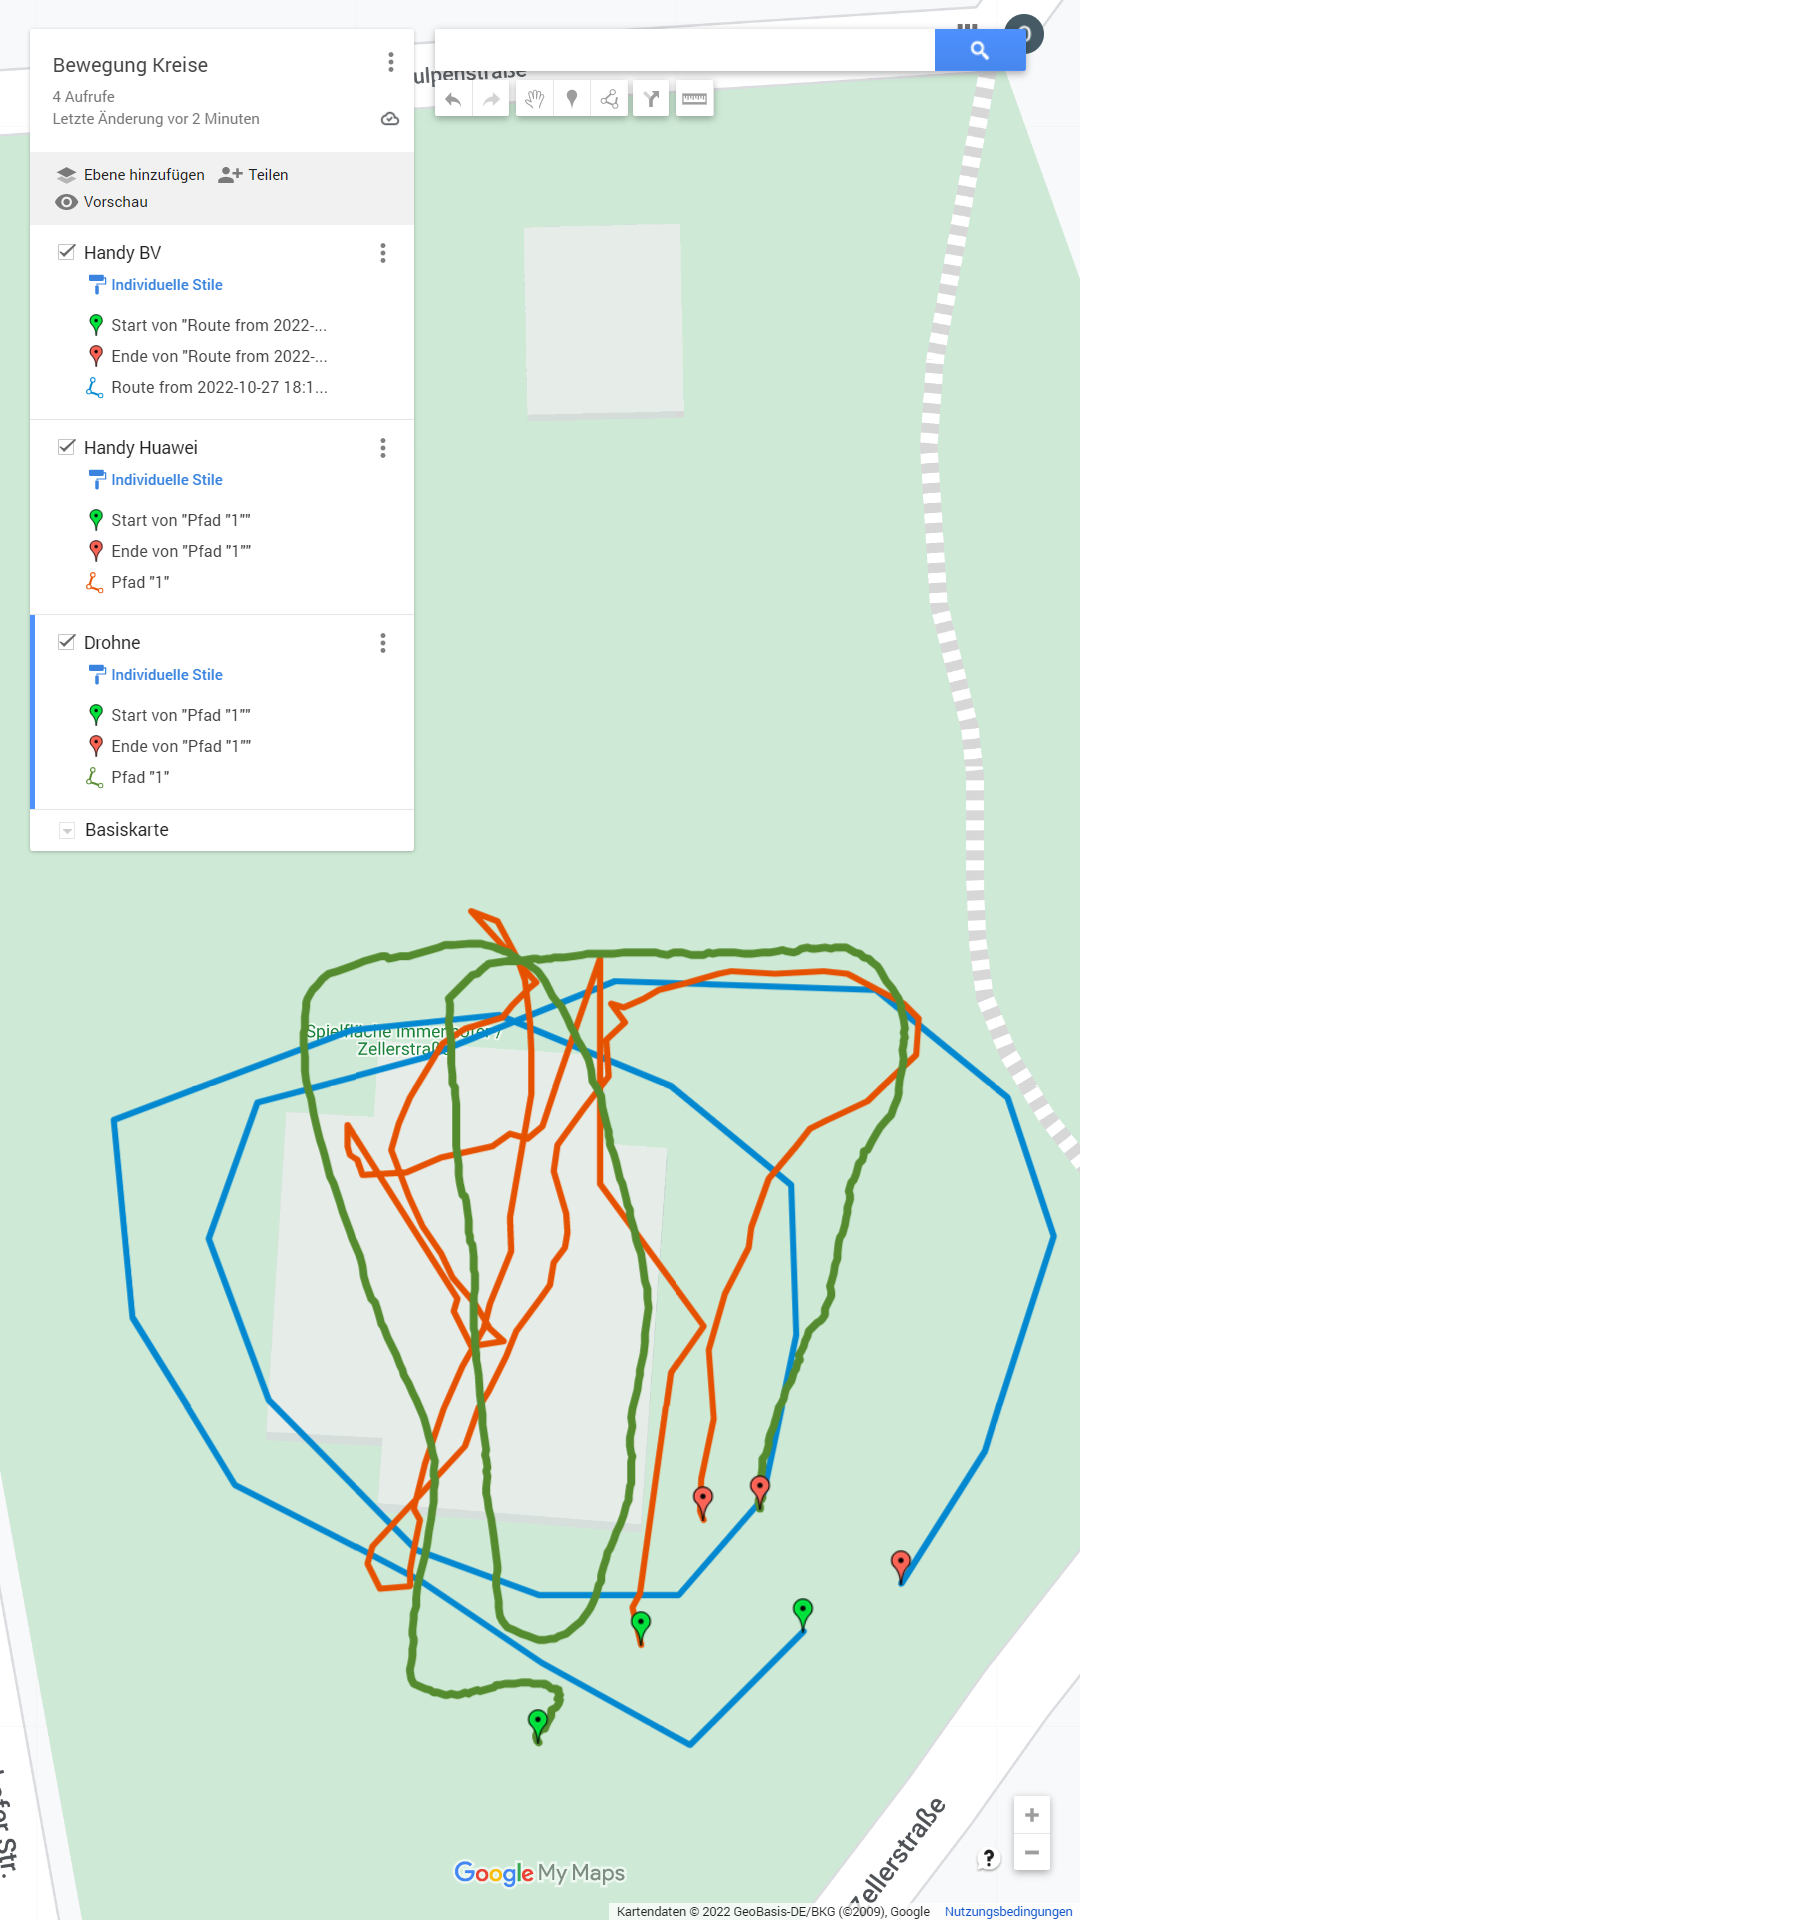
\includegraphics[width=0.5\textwidth]{images/lauf1.png}}
    \subfloat[Bewegung Bergab]{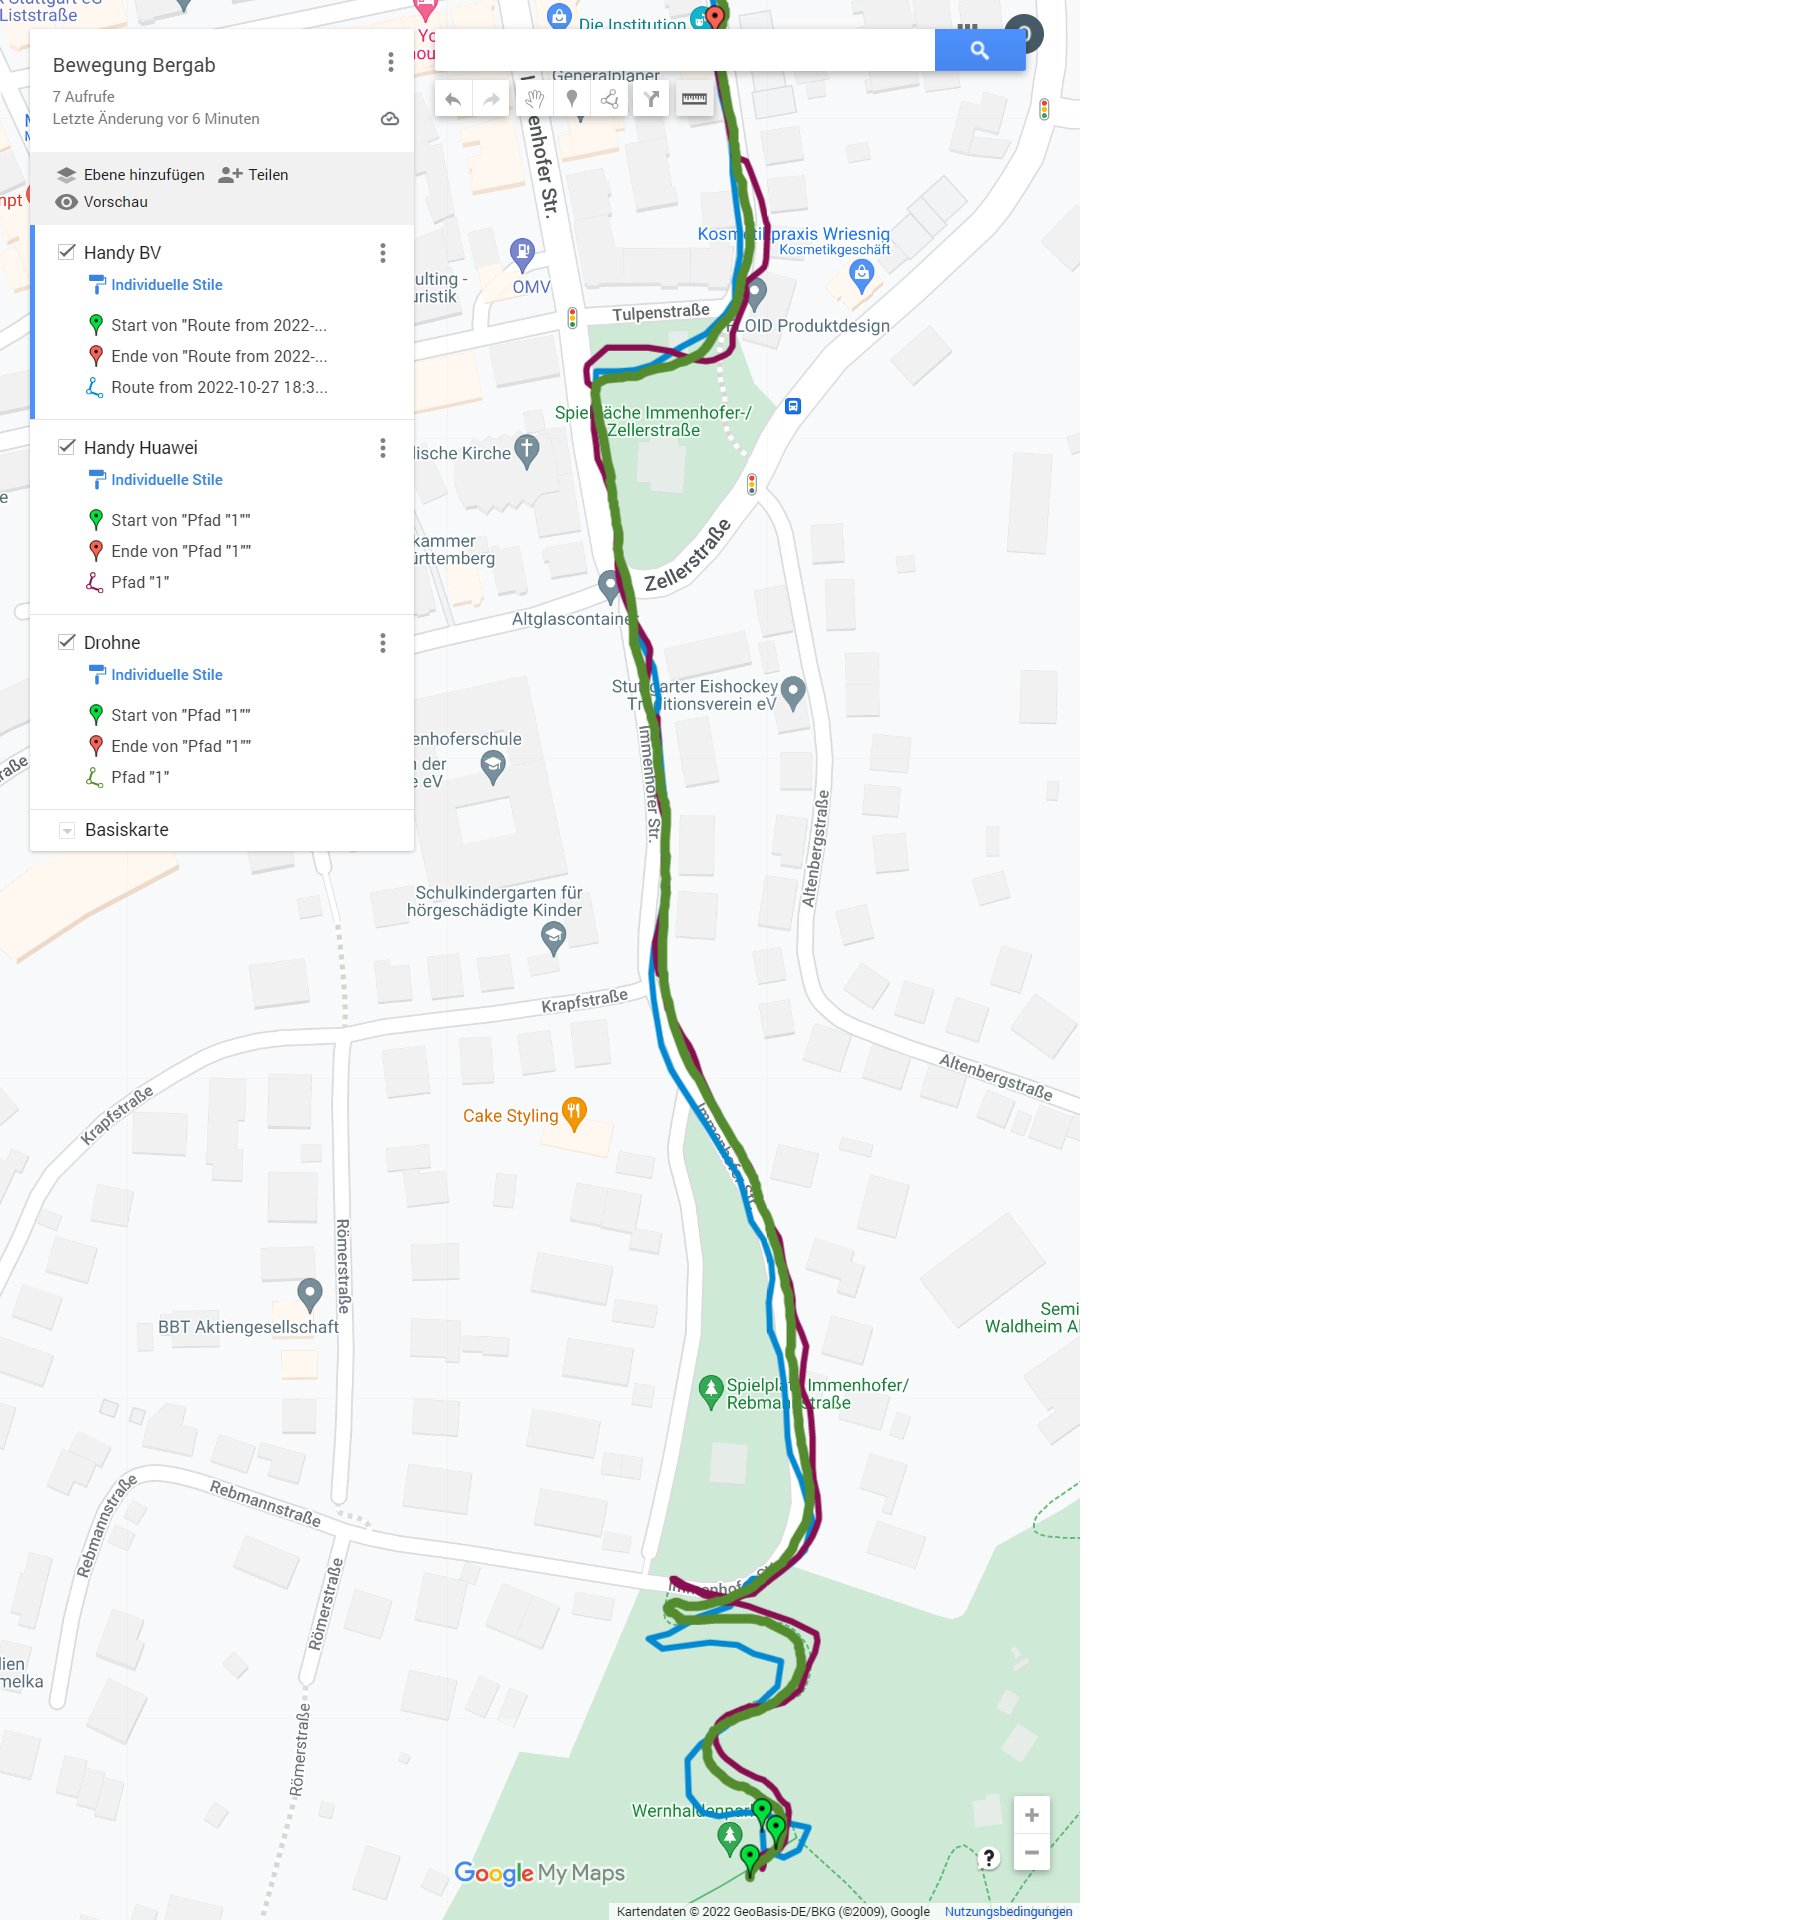
\includegraphics[width=0.5\textwidth]{images/lauf3.png}}
            
    \caption{Vergleich Bewegungsprofil verschiedener Geräte. GPS-Modul der Drohne in Grün, zwei Smartphones in Blau und Orange.}
    \label{fig:bench_gps}
\end{figure}

Weiterhin kann aus den GPS Daten Höhe, Geschwindigkeit und Neigung über die Zeit beobachtet werden. Die Drohne nimmt insgesamt mehr Messpunkte als die Smartphones auf, was ihr eine größere Genauigkeit und Zuverlässigkeit verleihen sollte. Auch gibt es bei den Smartphones teilweise Aussetzer bei der Aufzeichnung (entweder Signalverlust oder Software-Probleme). In Bild \ref{fig:bench_gps_elevation} zu sehen ist das Höhenprofil beim Bewegen der Drohne und eines Smartphones. Hätte die Drohne schwerwiegende Abweichungen während des Fluges könnte dies fatale Folgen haben. Auch ist das Profil der Drohne insgesamt ruhiger und glatter, was für gute Messwerte spricht.  

\begin{figure}[h!]
    \centering
    \subfloat[GPS-Modul Drohne]{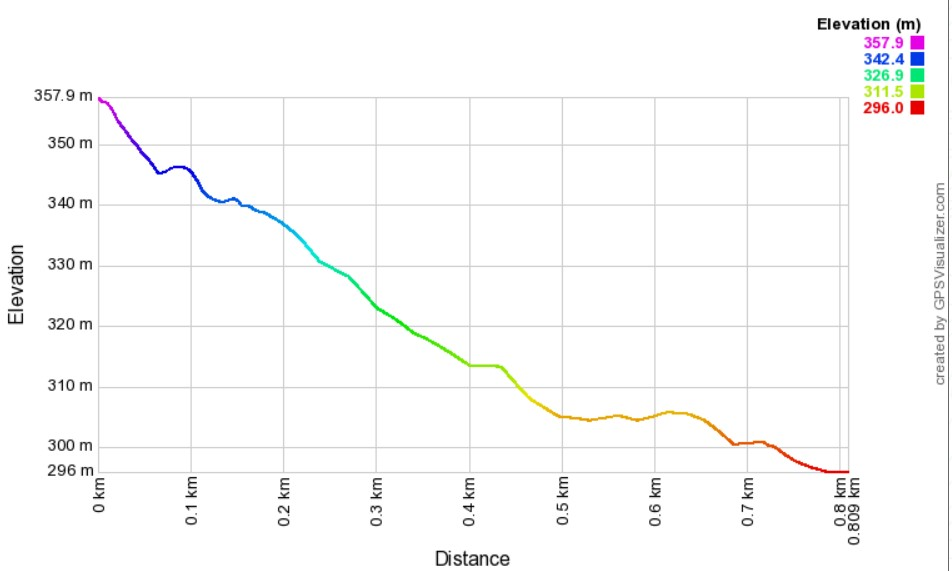
\includegraphics[width=0.5\textwidth]{images/lauf3_rpi_elevation.jpg}}
    \subfloat[Huawei-Smartphone]{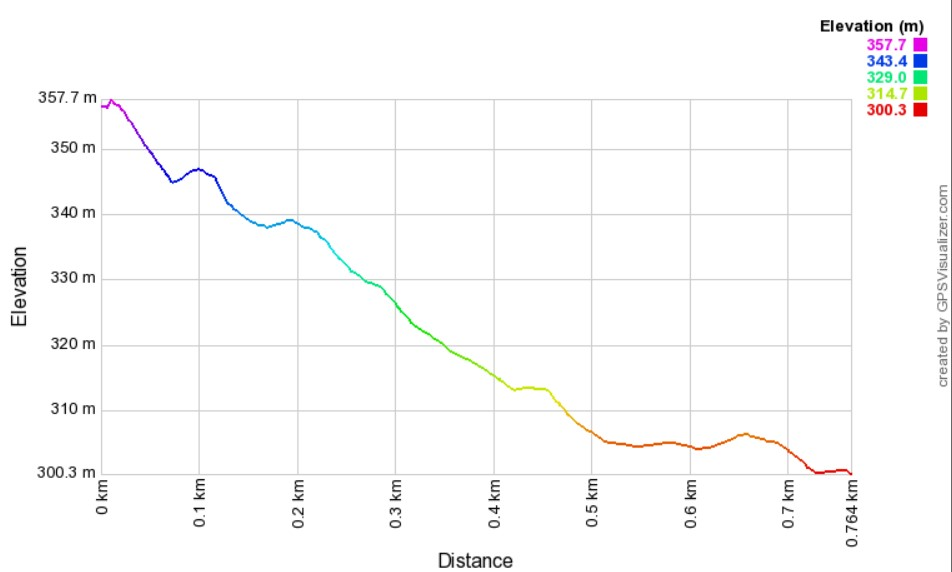
\includegraphics[width=0.5\textwidth]{images/lauf3_huawei_elevation.jpg}}
            
    \caption{Vergleich Höhenprofil verschiedener Geräte bei Bewegung bergab.}
    \label{fig:bench_gps_elevation}
\end{figure}

Um die Genauigkeit des GPS zu verbessern gibt es verschiedene Möglichkeiten\footnote{\url{https://ardupilot.org/copter/docs/common-rtk-correction.html}}. In der Praxis eingesetzt bei Landwirtschaftlichen Maschinen (Zentimetergenaue Fahrzeugführung) wird die zweite auf der Website aufgeführte Methode: über das Internet wird ein Korrektursignal abgerufen und dem GPS-Modul zugespielt. Diese Methode könnte auch einfach mithilfe des \gls{rpi} und einem GSM-Modul (Mobiles Internet über 3G) implementiert werden.

\subsection{Auslesen von Sensor-Daten}
Der Flugcontroller stellt verschiedene Sensoren bereit. Zusätzlich waren im ersten Projekt Ultraschallsensoren an den \gls{rpi} angeschlossenen. 

\subsubsection{Ultraschallsensoren am RPI}
Zuerst sollen die Ultraschall-Sensoren mit dem \gls{rpi} verbunden und getestet werden, um die Wiederverwendbarkeit zu bewerten. Derzeit sind an der Drohne 4 Ultraschallsensoren verbaut. Davon sind zwei nach vorn gerichtet, und jeweils einer nach oben und unten. Somit könnnen Objekte in der Flugbahn detektiert werden, solange die Bewegung entlang einer der Raumrichtungen: \enquote{Oben},\enquote{Unten} oder \enquote{Vorwärts} stattfindet. Zusammengesetzte Bewegungen dürften nicht durchgeführt werden, auch darf sich die Drohne nicht rückwärts bewegen.

In \cite[Kapitel 4.3.9]{wirthErweiterungBestehendenDrohne2022} ist beschrieben dass die Signale der Sensoren mit $5V$ anliegen, aber auf $3,3V$ herabgesetzt werden müssen um die Pins des \gls{rpi} nicht zu beschädigen.
Die Beschreibung sieht vor dazu einen Spannungsteiler einzusetzen. Bei genauem betrachten des Schaltplans fällt auf, dass der Spannungsteiler falsch gebaut wurde, und nicht die gewünschte Funktion erfüllt. Um die Pins des \gls{rpi} nicht doch zu beschädigen muss eine alternative Lösung gefunden werden. 

Weiterhin wurde ein Python-Script verwendet um die Pins am \gls{rpi} zu schalten/lesen. 
Zum anstoßen einer Messung soll das Trigger-Signal für $1\mu s$ auf \texttt{HIGH} (logisch 1) gesetzt werden. Um die Zeitverzögerung zu implementieren, wurde die Funktion \enquote{wait} verwendet. Eine Messung mit dem Oszilloskop zeigt, dass besagtes \enquote{wait} im Bereich von 200us liegt.\newline
Eine ähnliche Ungenauigkeit tritt beim Auslesen des ECHO-Signals auf. Die Bibliothek des \gls{rpi} wird verwendet um die Pins zu Pollen, was den Prozessor unnötig auslastet. Messungen mit konstant eingespeister Einschaltdauer (zu messendes Signal von Signalgenerator erzeugt) ergaben, dass immer 3 von 4 Messwerten gleich, der vierte aber eine Abweichung von ca. 8\% hatte.\\
Somit kann mit Python keine genaue Messung der Ultraschallsensoren durchgeführt werden. 

\paragraph*{Verwendung eines Aurduino zum Auslesen der Sensoren}
Zur Lösung der Problemene kann bspw. zusätzlich ein Arduino verwendet werden, der die Sensordaten korrekt ausliest und digitalisiert an den \gls{rpi} weiterleitet. Dies ist eine zuverlässige Lösung, erhöht aber auch gleichzeitig den Stromverbrauch. Um die Lösung einfach zu halten, wird diese trotzdem angewandt.

Zum Senden digitaler Messwerte muss ein Protokoll verwendet werden. Die UART-Pins des \gls{rpi} sind bereits mit dem Flugcontroller verbunden. Für den Anwendungszweck bietet sich das I2C-Protokoll an. Es erlaubt eine direkte Verbindung des Arduino mit dem \gls{rpi}, denn es werden vom Arduino keine $5V$ aktiv geschalten sondern nur der Leitungsbus auf Masse heruntergezogen.

Die Ultraschallsensoren\footnote{\url{https://cdn.sparkfun.com/datasheets/Sensors/Proximity/HCSR04.pdf}} haben eine Reichweite von ca. $2cm$ bis $4m$ und eine Genauigkeit von ca. $3mm$. Für die Entwicklung wird die maximale Distanz auf $3.8m$ festgelegt. Es wird ein kleinerer Wert als im Datenblatt angenommen, da der Idealwert nur bei stillstehenden glatten Flächen erreicht werden kann. Im Datenblatt wird empfohlen, zwischen aufeinanderfolgenden Messungen mindestens $60ms$ abzuwarten, um Fehleinstreuungen durch weitere Ultraschallechos zu vermeiden. Um weitere Fehler zu vermeiden wird diese Zeit vorerst auch zwischen den Messungen der 4 Sensoren eingehalten. Eine weitere Verzögerung entsteht durch das Messen selbst (maximal $\frac{380cm}{0.5 \times 0.034\frac{cm}{s}}\approx 22352\mu s$), diese wird vorsorglich von der jeweiligen Wartezeit abgezogen. Die minimale Periode der Sensordaten beträgt somit $4 \times 60ms=240ms$. Grob gesagt, entspricht die Frequenz der Sensordaten somit $4Hz$.
%Dies ist nicht gerade hoch und könnte bei schnellen Flügen leicht zu Fehlern führen.

Ein weiteres Problem ist das durch die Ultraschallsensoren verursachte Rauschen der Messwerte. Bei Messungen im Raum mit konstantem Abstand zu Obejekten ergaben sich Abweichungen zwischen 2 Messungen von ca. $1\%-2\%$, siehe Bild \ref{fig:ultrasonic_noise}, \ref{fig:ultrasonic_scatter}. Im linken Bild sind nacheinander die Messwerte mehrerer Ultraschallsensoren aufgeführt, das rechte Bild zeigt den zeitlichen Verlauf von Messdaten. Selbst bei Stillstand (Anfang und Ende der Messung) sind Schwankungen in den Messwerten zu sehen.

Auch haben die Ultraschallsensoren ein Problem mit Bewegungen. In Bild \ref{fig:ultrasonic_scatter} wurde der Sensor zuerst in Richtung Decke gehalten (Beginn bei ca. $8s$ auf der x-Achse). Dann wurde er waagerecht gedreht, in den Raum zeigend. Kann der Sensor keinen Wert erfassen, kommt es auf dem Arduino zu einem Timeout und es wird $0$ zurückgegeben (ca. bei $11s$). Zu beachten sind die starken Abweichungen während den Bewegungen: es kommt immer wieder zu starken Einbrüchen und Anstiegen (bspw. bei $14s$) durch teilweisen Verlust des Echo-Signals.

\begin{figure}[h!]
    \centering
    \subfloat[Nacheinander ausgelesene Sensordaten]{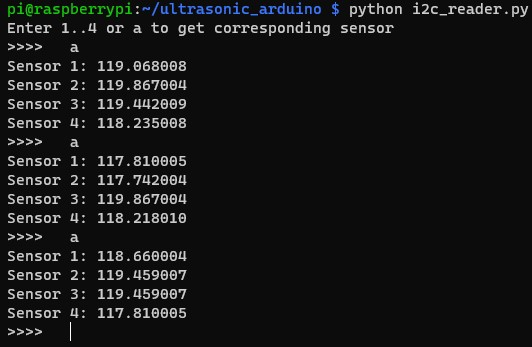
\includegraphics[width=0.5\textwidth]{images/bench_ultrasonic_noise.jpg}\label{fig:ultrasonic_noise}}
    \subfloat[Verhalten bei Bewegung eines Sensors]{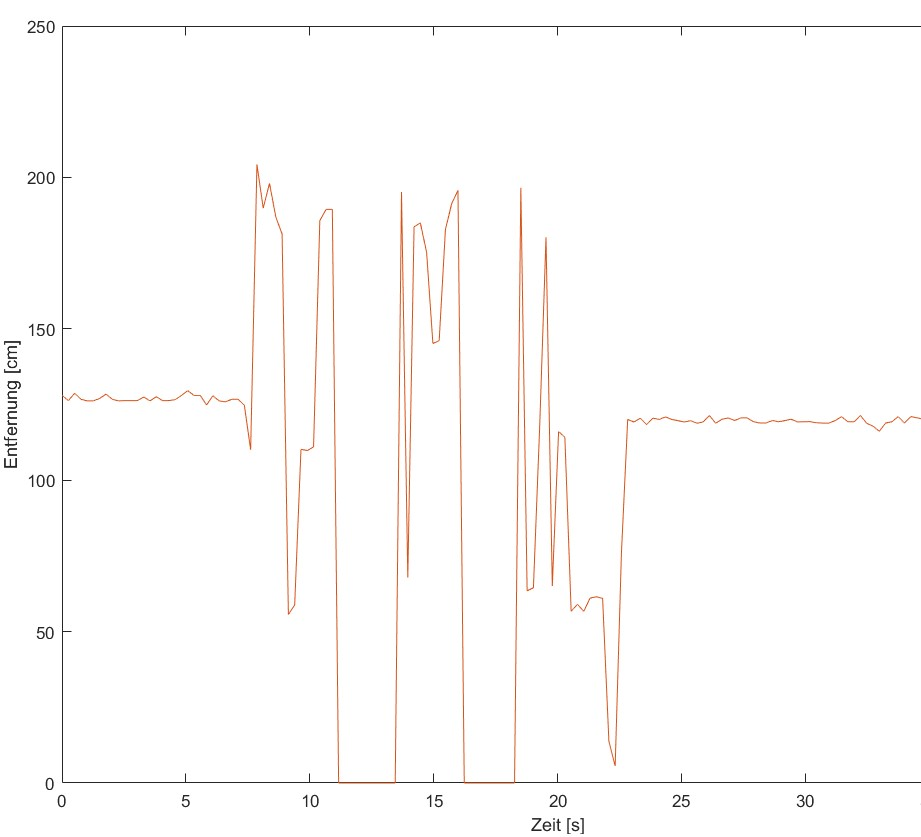
\includegraphics[width=0.5\textwidth]{images/bench_ultrasonic_movement_scatter.jpg}\label{fig:ultrasonic_scatter}}

    \caption{Demonstration der Ultraschallsensoren}
    \label{fig:ultrasonic_tests}
\end{figure}

Durch den Feldversuch wird ersichtlich, dass Ultraschallsensoren nur funktionieren, wenn sie nahezu senkrecht auf Flächen gerichtet werden. Somit können auch keine Hindernisse (wie bspw. Wände) detektiert werden, auf die sich die Drohne schräg zubewegt. Nicht messbare Entfernungen (zu nahe oder zu große Entfernung) werden beim weiteren Vorgehen durch die Entfernung von $4m$ ersetzt und die maximal messbare Entfernung der Sensoren auf $3m$ begrenzt.

Um die Messwerte der Sensoren sinnvoll verarbeiten zu können ist weiteres Filtern notwendig. Eine einfache Implementation für einen Filter sind Moving Average Filter, oder speziell für diesen Anwendungszweck, wie in \footnote{\url{https://renegaderobotics.org/filtering-sensor-data/}} beschriebene Median Filter. Bei dem zuletzt beschriebenen Verfahren werden manuell Grenzen festgelegt, welche Messwerte gefiltert werden müssen. Für die Messungen wurden Abweichungen kleiner 1\% ignoriert und größer 3\% gefiltert. Vom beschriebenen Vorgehen zum filtern wurde aber abgeichen und anstatt des Medians jeweils der Mittelwert der letzten Messwerte, gespeichert in einem Filter-Array, errechnet. In Bild \ref{fig:ultrasonic_filters} ist eine weitere Messung dargestellt. Die besten Resultate (wenige Sprünge, steile Anstiege) liefert der \enquote{Median Filter 1} und soll im Projekt weiterhin verwendet werden.

\begin{figure}[!h]
	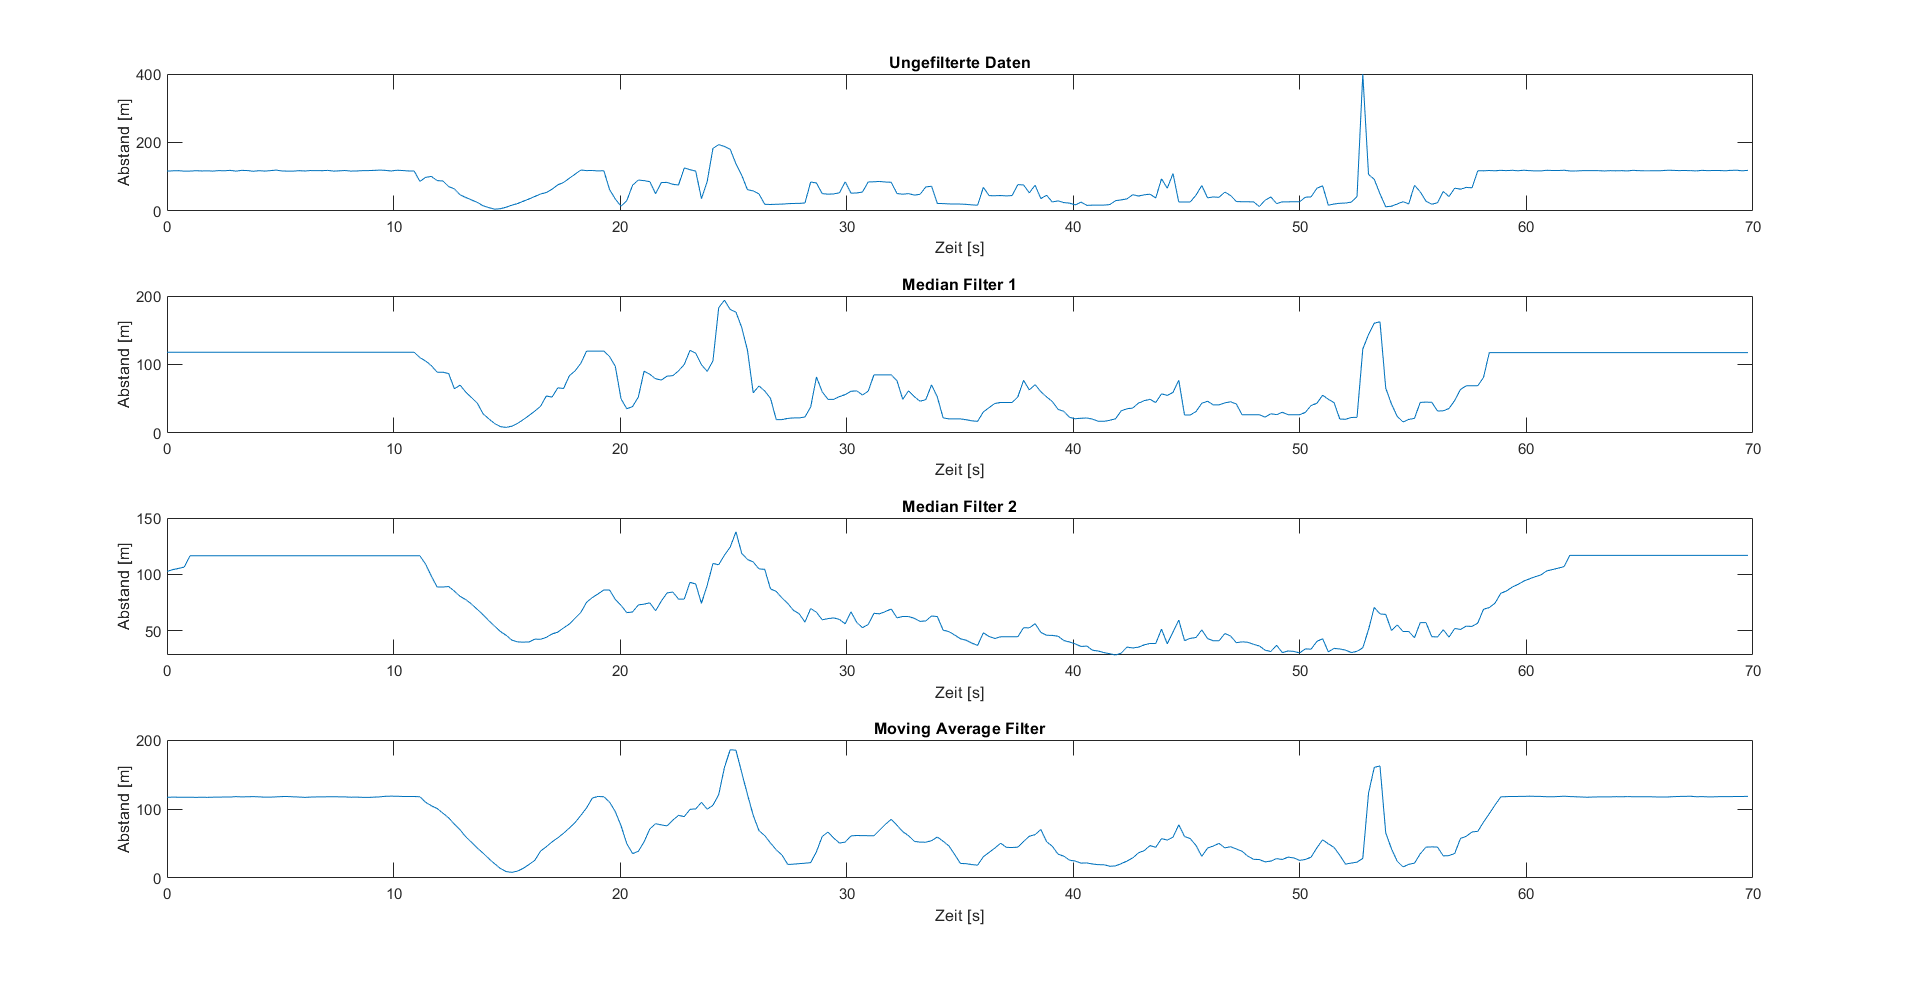
\includegraphics[width=\linewidth]{images/ultrasonic_cmp_filter.png}
	\caption{Messung mit einem Ultraschallsensor. Zu sehen: oben ungefilterte Messwerte; Median Filter 1 pflegt Sprünge in Messdaten direkt in Filter-Array ein aber berechnet Durchschnitt; Median Filter 2 pflegt berechneten Durchschnittswert in Filter-Array ein; Moving Average berechnet immer den Durchschnittswert der vergangenen Messwerte.}
	\label{fig:ultrasonic_filters}
  \end{figure} 

[TODO: neue Bibliothek entwerfen, am besten gleich mit ROS]

\subsubsection{Einspeisen von Parameterwerten der Drohne für ROS}

[TODO: vielliecht gibt es schon eine "direkte Einspeisung", muesste ich mich mal belesen]
[TODO: Alternativ kann der Flugcontroller auch einen EKF berechnen]


\clearpage
\appendix
%% !TeX spellcheck = de_DE
%Die Angabe des schlauen Spruchs auf diesem Wege funtioniert nur,
%wenn keine Änderung des Kapitels mittels den in preambel/chapterheads.tex
%vorgeschlagenen Möglichkeiten durchgeführt wurde.
\setchapterpreamble[u]{%
\dictum[Albert Einstein]{Probleme kann man niemals mit derselben Denkweise lösen, durch die sie entstanden sind.}
}

\chapter{LaTeX-Tipps}
\label{chap:latextipps}

Pro Satz eine neue Zeile.
Das ist wichtig, um sauber versionieren zu können.
In LaTeX werden Absätze durch eine Leerzeile getrennt.

Folglich werden neue Abstäze insbesondere \emph{nicht} durch Doppelbackslashes erzeugt.
Der letzte Satz kam in einem neuen Absatz.

\section{File-Encoding und Unterstützung von Umlauten}
\label{sec:firstsectioninlatexhints}
Die Vorlage wurde 2010 auf UTF-8 umgestellt.
Alle neueren Editoren sollten damit keine Schwierigkeiten haben.

\section{Zitate}
Referenzen werden mittels \texttt{\textbackslash cite[key]} gesetzt.
Beispiel: \cite{WSPA} oder mit Autorenangabe: \citet{WSPA}.

Der folgende Satz demonstriert \begin{inparaenum}[1.]
\item die Großschreibung von Autorennamen am Satzanfang,
\item die richtige Zitation unter Verwendung von Autorennamen und der Referenz,
\item dass die Autorennamen ein Hyperlink auf das Literaturverzeichnis sind sowie
\item dass in dem Literaturverzeichnis der Namenspräfix \enquote{van der} von \enquote{Wil M.\,P.\ van der Aalst} steht.
\end{inparaenum}
\Citet{RVvdA2016} präsentieren eine Studie über die Effektivität von Workflow-Management-Systemen.

Der folgende Satz demonstriert, dass man mittels \texttt{label} in einem Bibliopgrahie"=Eintrag den Textteil des generierten Labels überschreiben kann, aber das Jahr und die Eindeutigkeit noch von biber generiert wird.
Die Apache ODE Engine \cite{ApacheODE} ist eine Workflow-Maschine, die BPEL-Prozesse zuverlässig ausführt.

Wörter am besten mittels \texttt{\textbackslash enquote\{...\}} \enquote{einschließen}, dann werden die richtigen Anführungszeichen verwendet.

Beim Erstellen der Bibtex-Datei wird empfohlen darauf zu achten, dass die DOI aufgeführt wird.

\section{Mathematische Formeln}
\label{sec:mf}
Mathematische Formeln kann man $so$ setzen. \texttt{symbols-a4.pdf} (zu finden auf \url{http://www.ctan.org/tex-archive/info/symbols/comprehensive/symbols-a4.pdf}) enthält eine Liste der unter LaTeX direkt verfügbaren Symbole.
Z.\,B.\ $\mathbb{N}$ für die Menge der natürlichen Zahlen.
Für eine vollständige Dokumentation für mathematischen Formelsatz sollte die Dokumentation zu \texttt{amsmath}, \url{ftp://ftp.ams.org/pub/tex/doc/amsmath/} gelesen werden.

Folgende Gleichung erhält keine Nummer, da \texttt{\textbackslash equation*} verwendet wurde.
\begin{equation*}
x = y
\end{equation*}

Die Gleichung~\ref{eq:test} erhält eine Nummer:
\begin{equation}
\label{eq:test}
x = y
\end{equation}

Eine ausführliche Anleitung zum Mathematikmodus von LaTeX findet sich in \url{http://www.ctan.org/tex-archive/help/Catalogue/entries/voss-mathmode.html}.

\section{Quellcode}
\Cref{lst:ListingANDlstlisting} zeigt, wie man Programmlistings einbindet.
Mittels \texttt{\textbackslash lstinputlisting} kann man den Inhalt direkt aus Dateien lesen.

%Listing-Umgebung wurde durch \newfloat{Listing} definiert
\begin{Listing}
\begin{lstlisting}
<listing name="second sample">
  <content>not interesting</content>
</listing>
\end{lstlisting}
\caption{lstlisting in einer Listings-Umgebung, damit das Listing durch Balken abgetrennt ist}
\label{lst:ListingANDlstlisting}
\end{Listing}

Quellcode im \lstinline|<listing />| ist auch möglich.

\section{Abbildungen}

Die \cref{fig:chor1} und \ref{fig:chor2} sind für das Verständnis dieses Dokuments wichtig.
Im Anhang zeigt \vref{fig:AnhangsChor} erneut die komplette Choreographie.

%Die Parameter in eckigen Klammern sind optionale Parameter - z.B. [htb!]
%htb! bedeutet: "Liebes LaTeX, bitte platziere diese Abbildung zuerst hier ("_h_ere"). Falls das nicht funktioniert, dann bitte oben auf der Seite ("_t_op"). Und falls das nicht geht, bitte unten auf der Seite ("_b_ottom"). Und bitte, bitte bevorzuge hier und oben, auch wenn's net so optimal aussieht ("!")
%Diese sollten nach Möglichkeit NICHT verwendet werden. LaTeX's Algorithmus für das Platzieren der Gleitumgebung ist schon sehr gut!
\begin{figure}
  \centering
  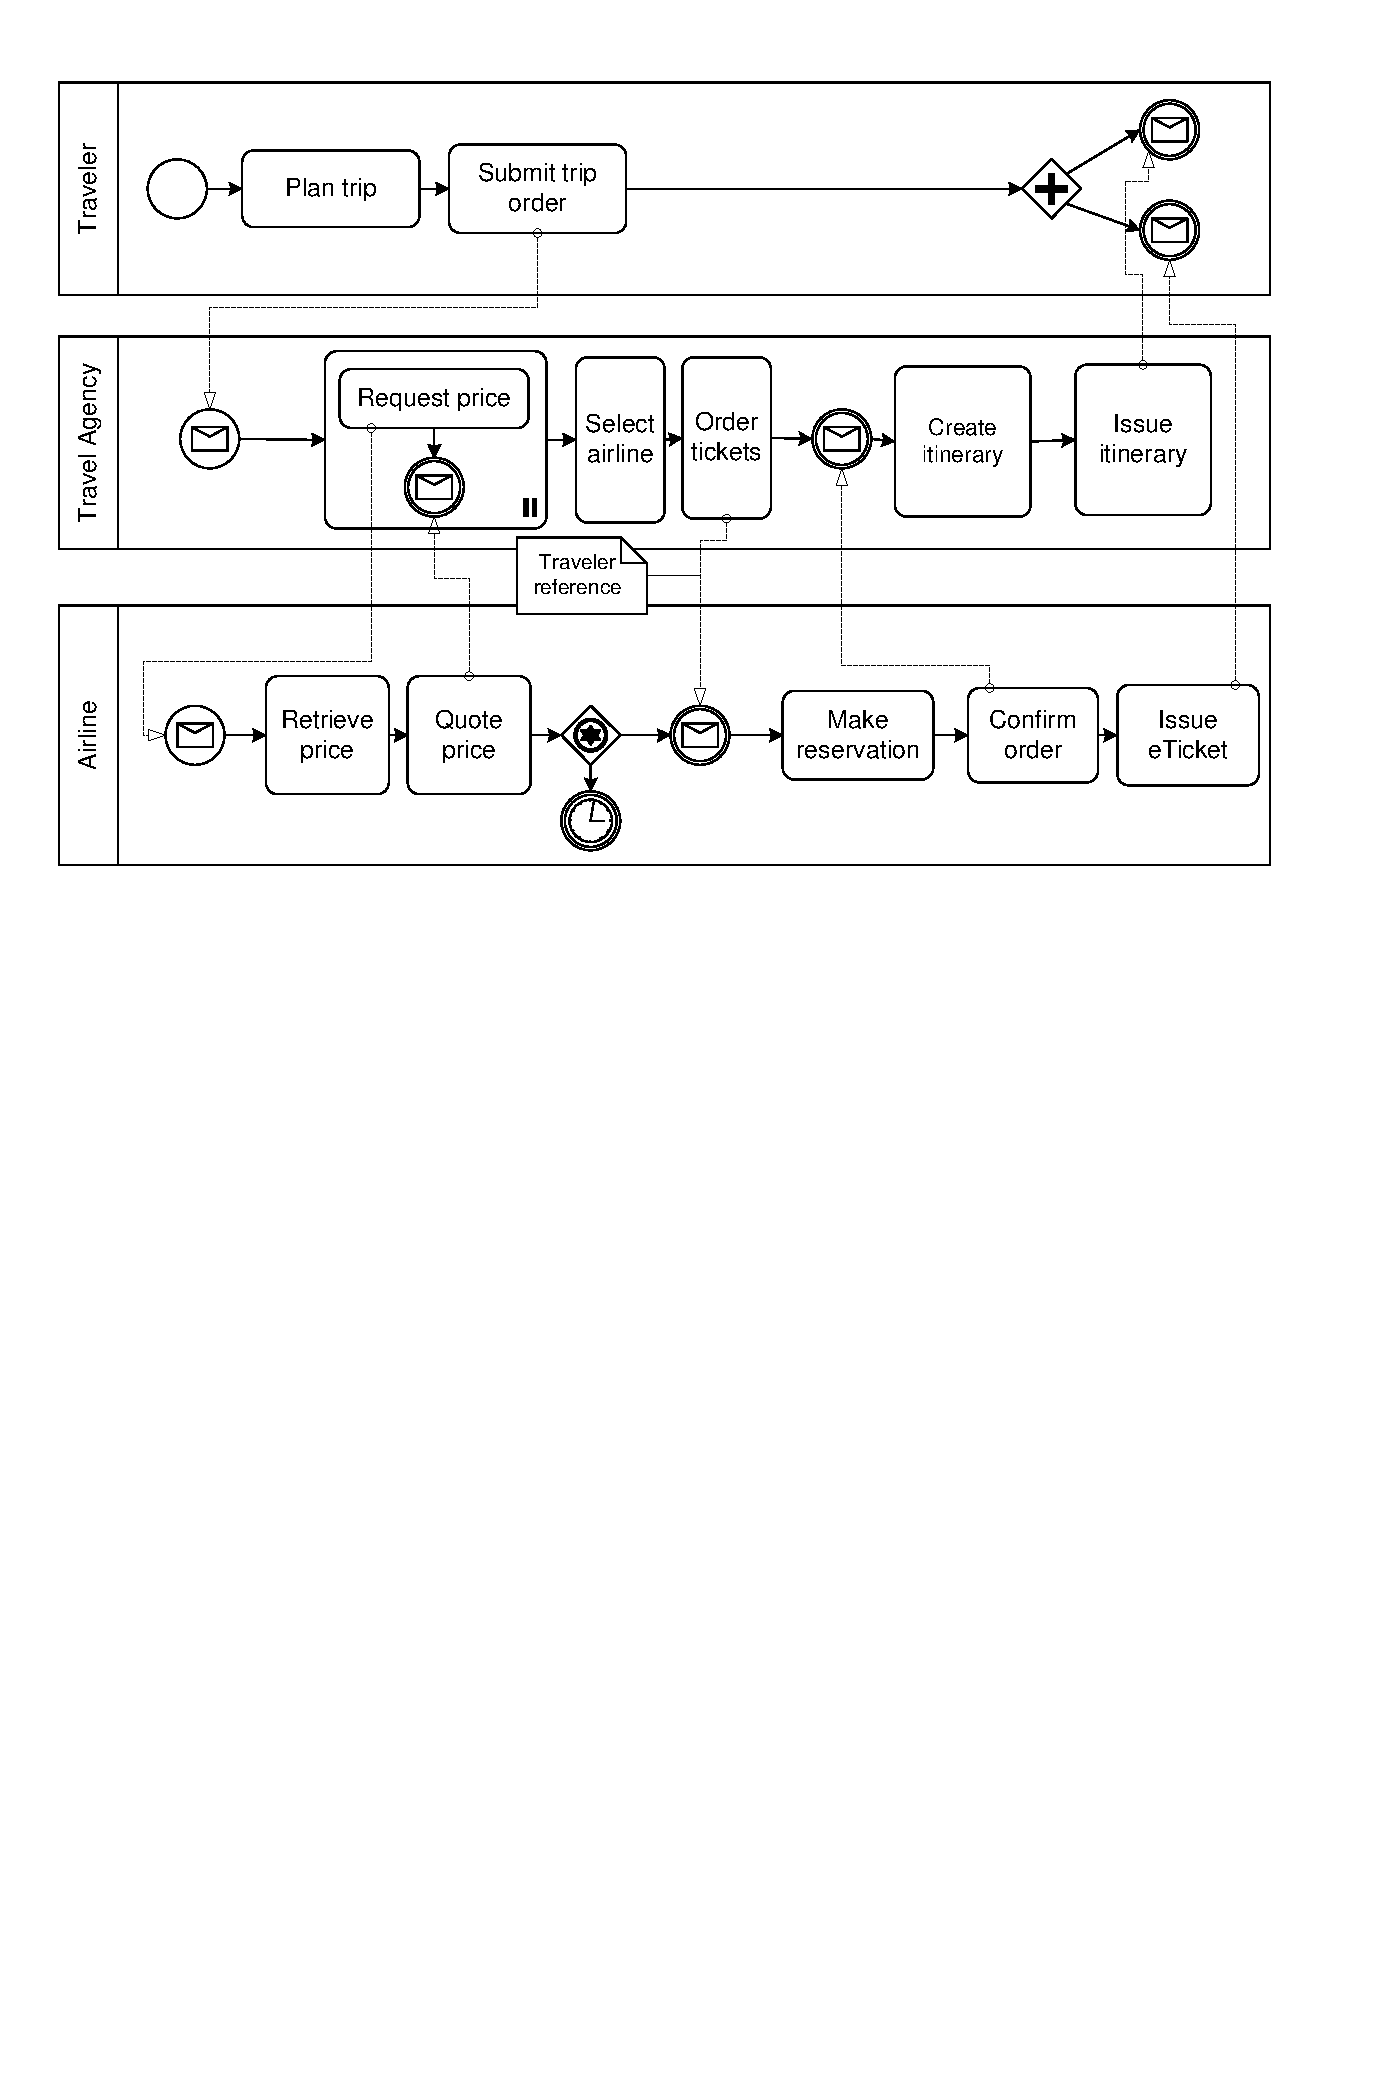
\includegraphics[width=\textwidth]{choreography.pdf}
  \caption{Beispiel-Choreographie}
  \label{fig:chor1}
\end{figure}

\begin{figure}
  \centering
  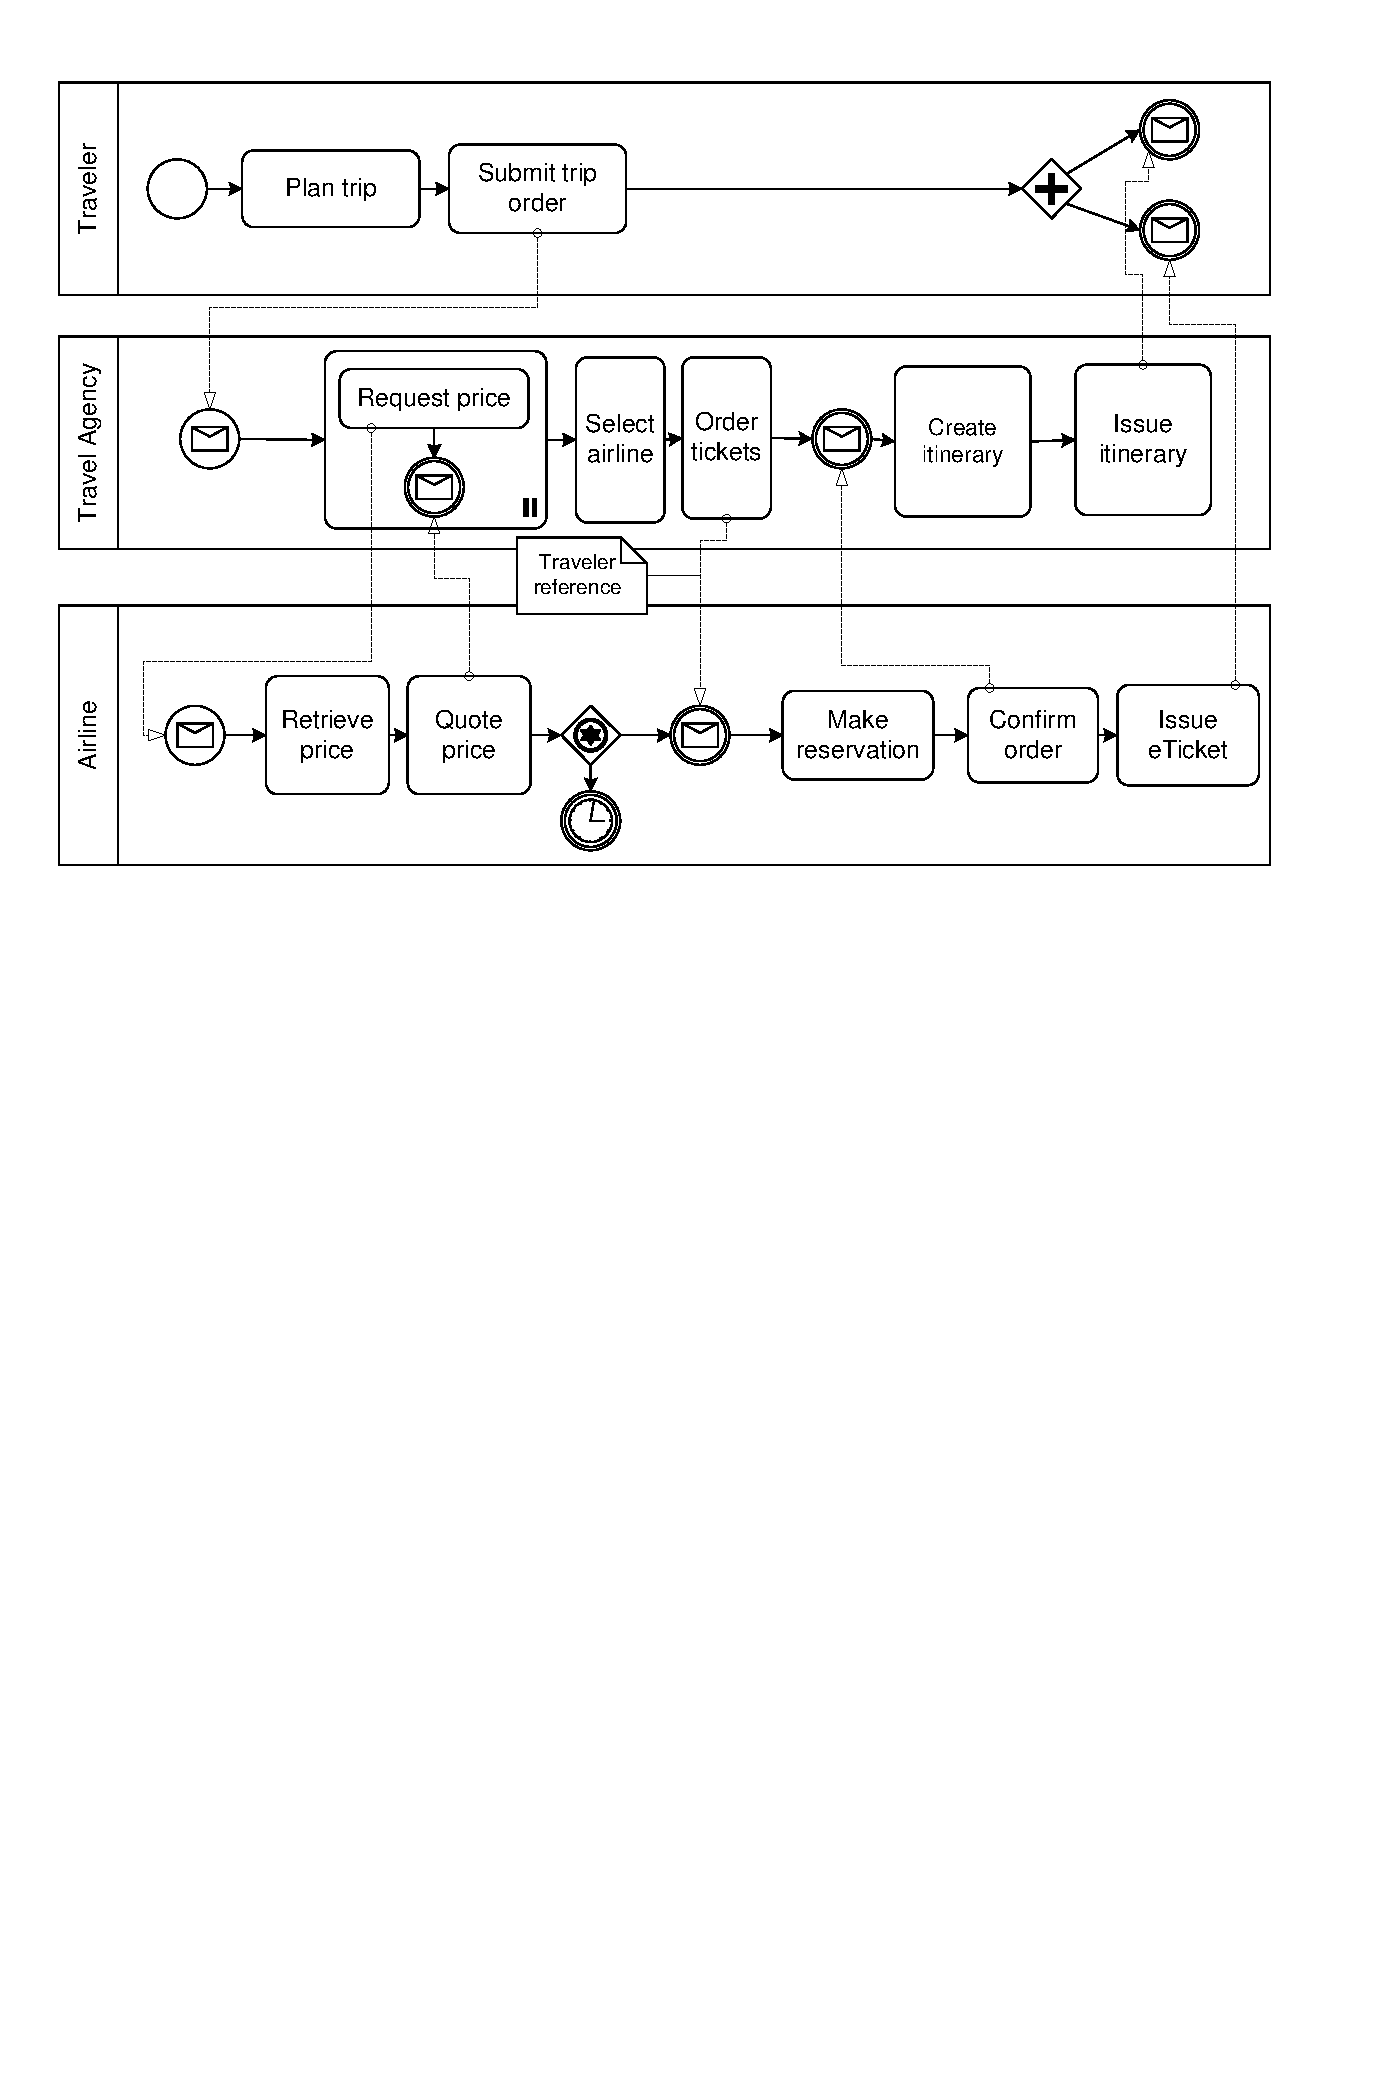
\includegraphics[width=.8\textwidth]{choreography.pdf}
  \caption[Beispiel-Choreographie]{Die Beispiel-Choreographie. Nun etwas kleiner, damit \texttt{\textbackslash textwidth} demonstriert wird. Und auch die Verwendung von alternativen Bildunterschriften für das Verzeichnis der Abbildungen. Letzteres ist allerdings nur Bedingt zu empfehlen, denn wer liest schon so viel Text unter einem Bild? Oder ist es einfach nur Stilsache?}
  \label{fig:chor2}
\end{figure}


\begin{figure}
  \centering
    \subfloat[]{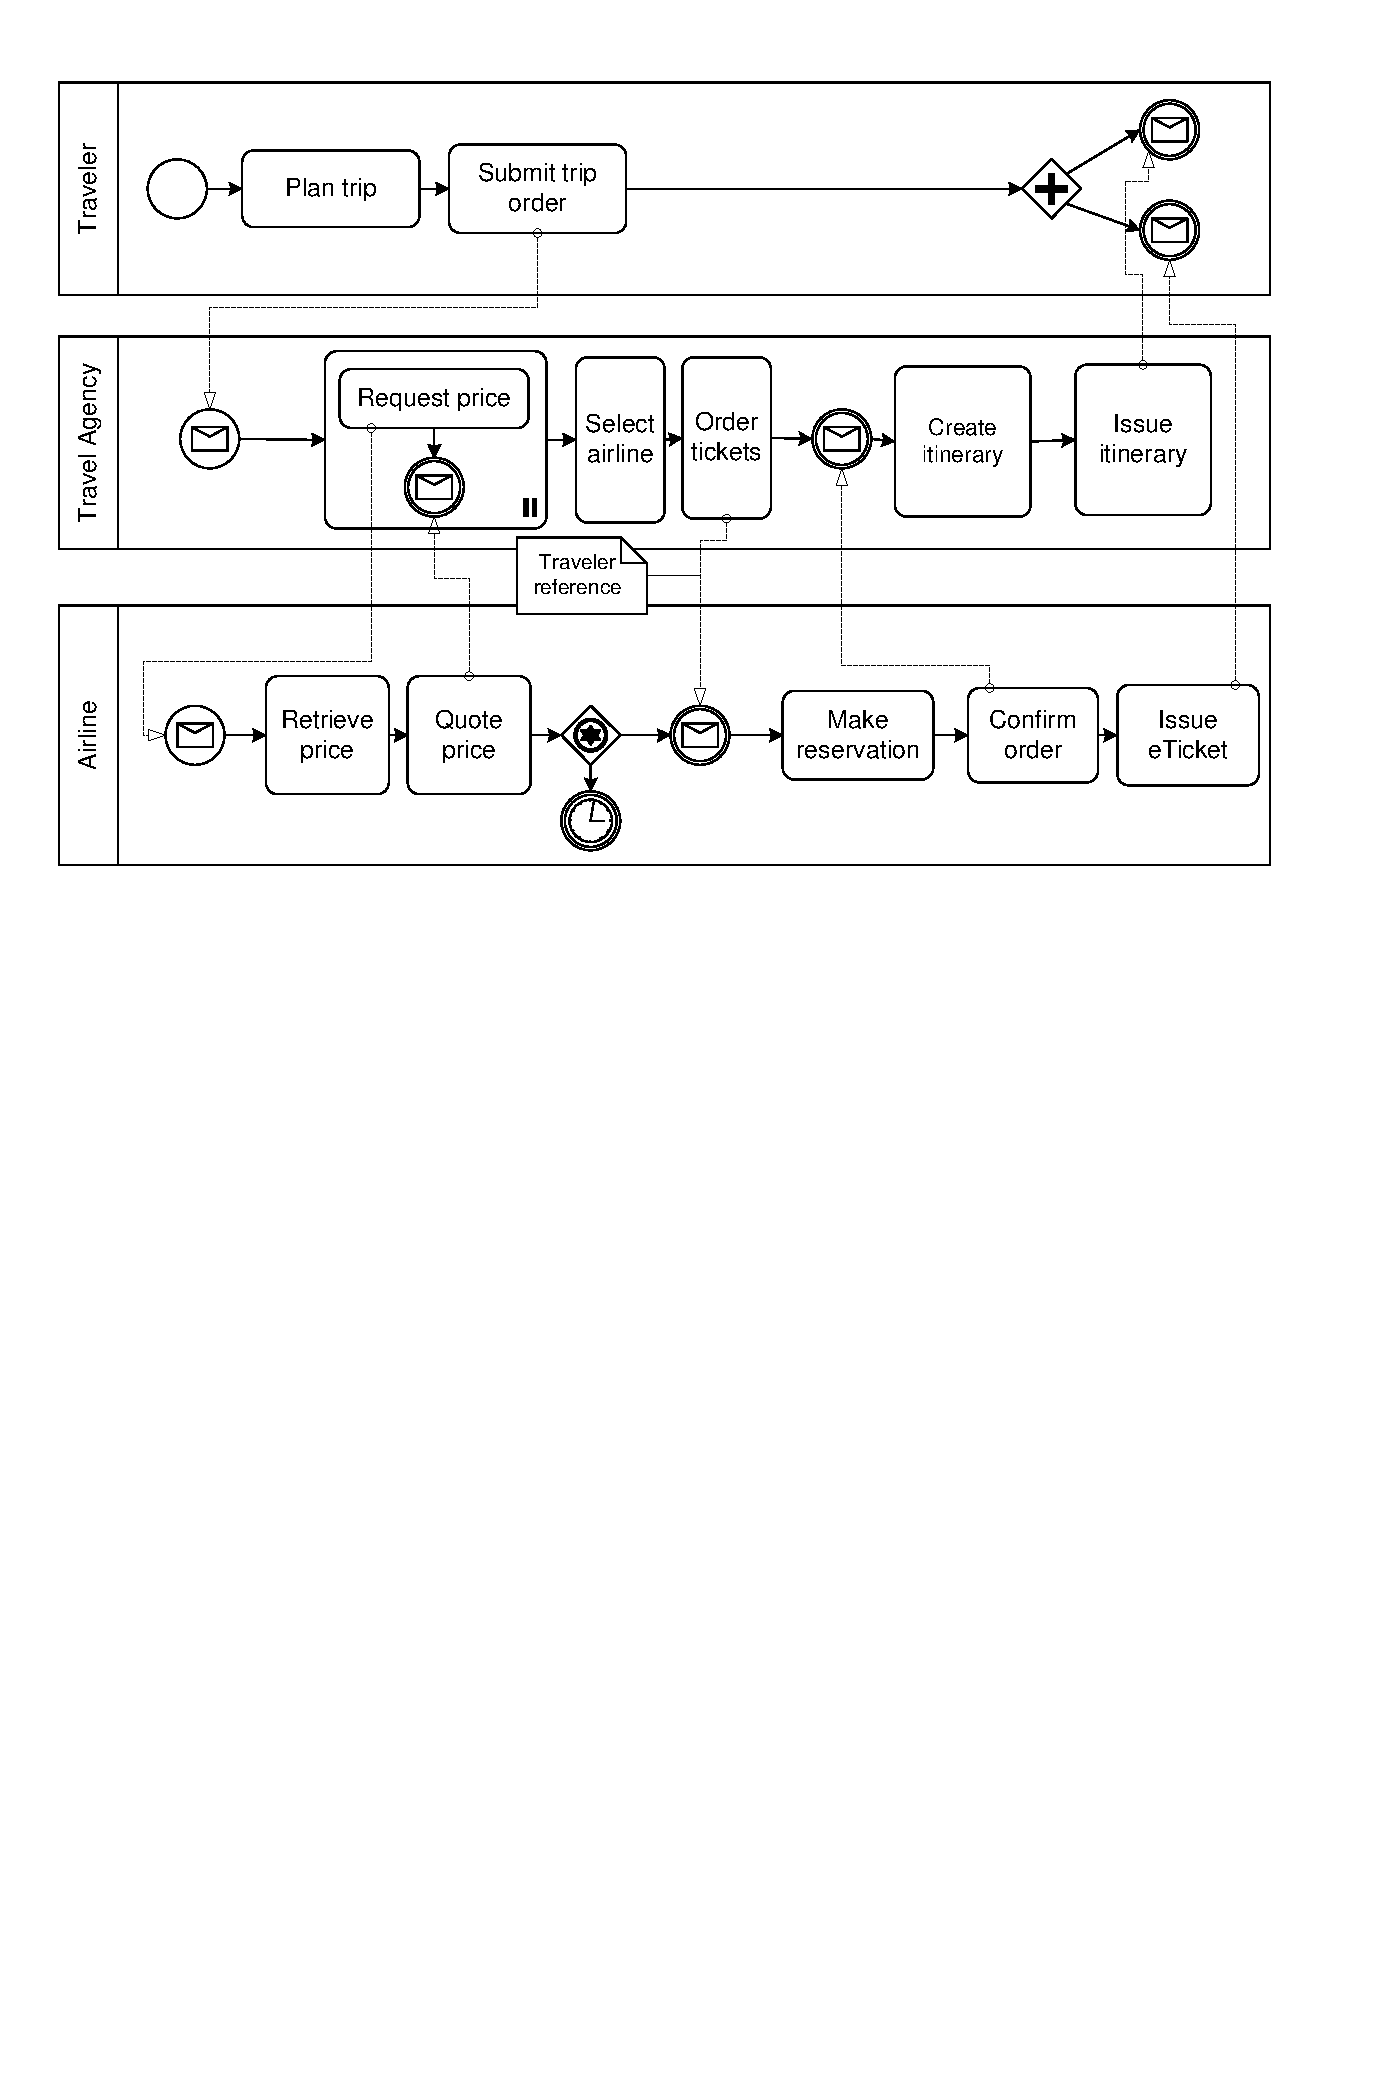
\includegraphics[width=0.3\textwidth]{choreography.pdf} \label{fig:subfigA}}
    \subfloat[]{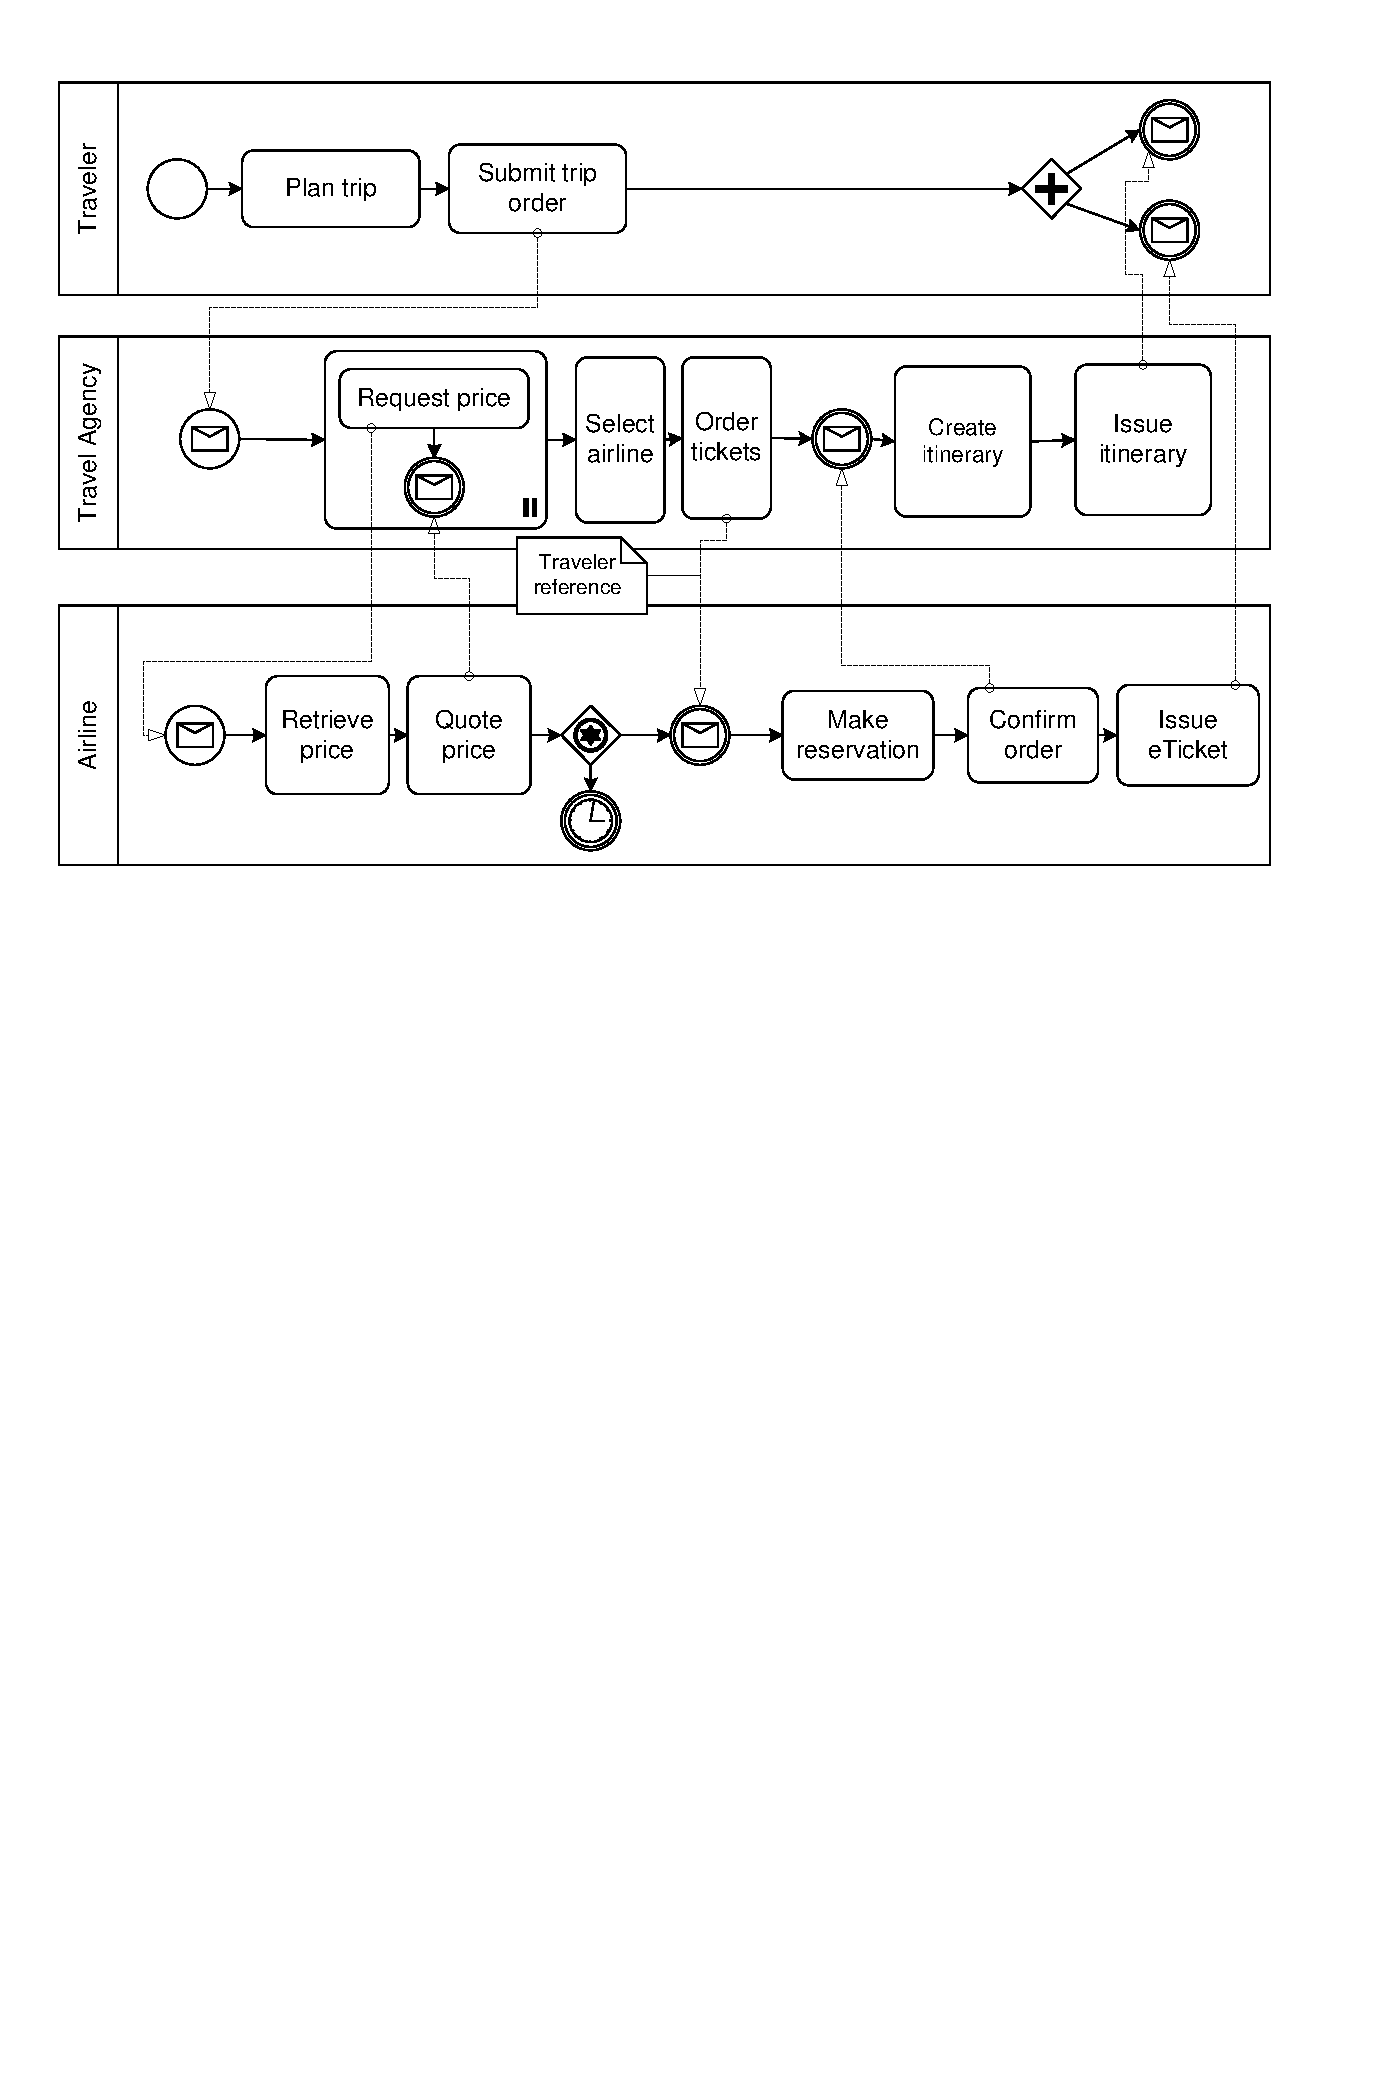
\includegraphics[width=0.3\textwidth]{choreography.pdf} \label{fig:subfigB}}
		\subfloat[Subcaption if needed]{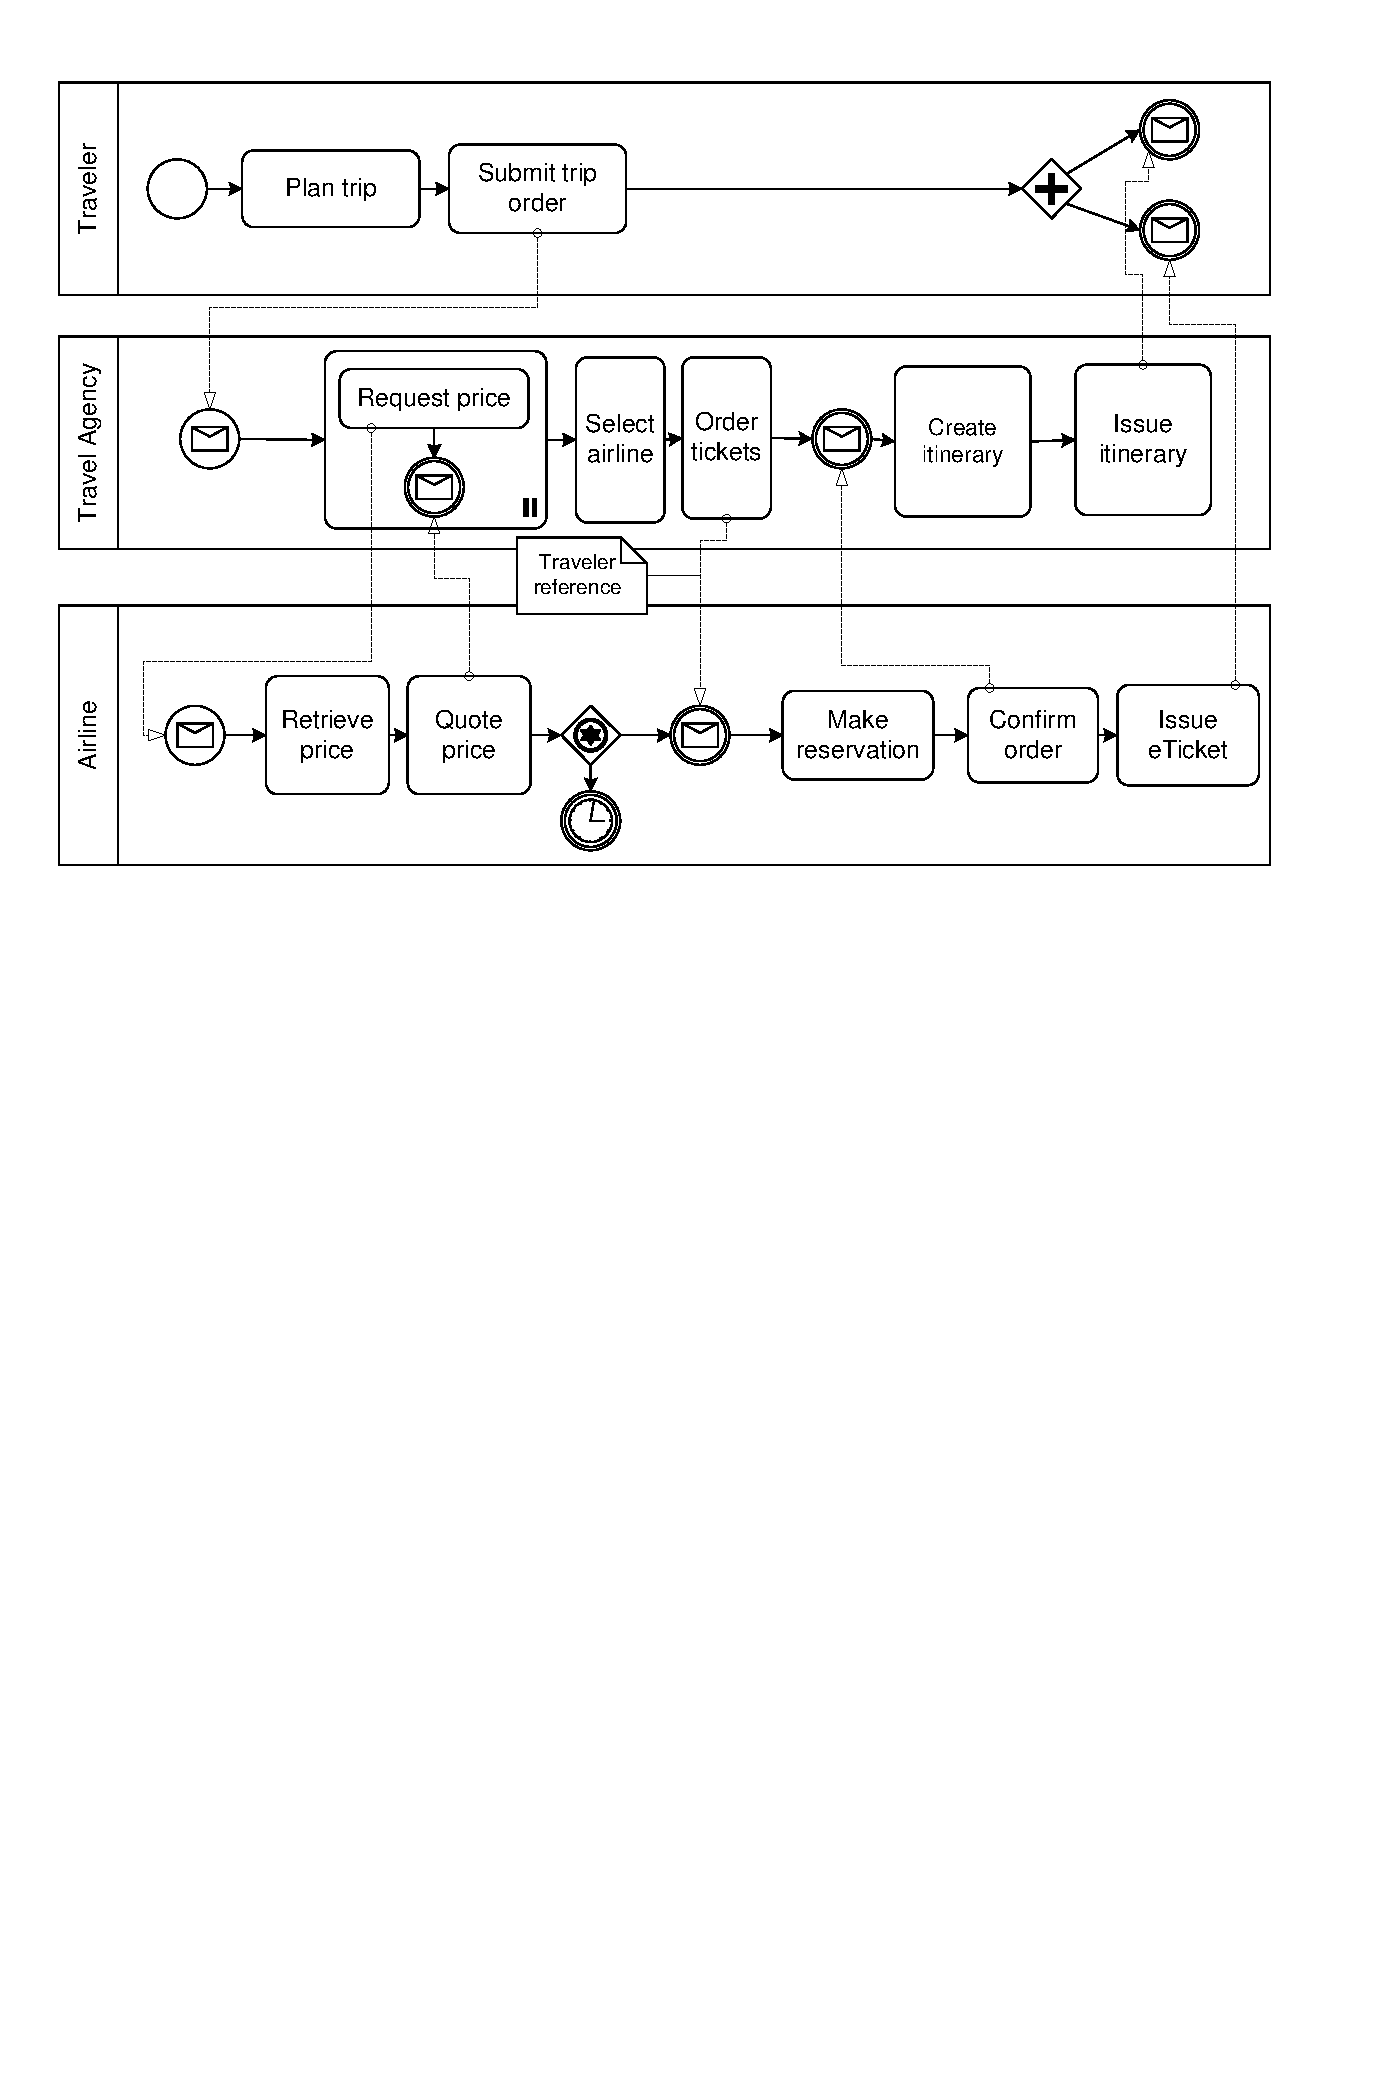
\includegraphics[width=0.3\textwidth]{choreography.pdf} \label{fig:subfigC}}
	\caption{Beispiel um 3 Abbildung nebeneinader zu stellen nur jedes einzeln referenzieren zu können. Abbildung~\ref{fig:subfigB}
 ist die mittlere Abbildung.}
\label{fig:subfig_example}
\end{figure}

Es ist möglich, SVGs direkt beim Kompilieren in PDF umzuwandeln.
Dies ist im Quellcode zu latex-tipps.tex beschrieben, allerdings auskommentiert.

\iffalse % <-- Das hier wegnehmen, falls inkscape im Pfad ist
Das SVG in \cref{fig:directSVG} ist direkt eingebunden, während der Text im SVG in \cref{fig:latexSVG} mittels pdflatex gesetzt ist.
Falls man die Graphiken sehen möchte, muss inkscape im PATH sein und im Tex-Quelltext \texttt{\textbackslash{}iffalse} und \texttt{\textbackslash{}iftrue} auskommentiert sein.

\begin{figure}
\centering

\includegraphics{svgexample.svg}
\caption{SVG direkt eingebunden}
\label{fig:directSVG}
\end{figure}

\begin{figure}
\centering
\def\svgwidth{.4\textwidth}
\includesvg{svgexample}
\caption{Text im SVG mittels \LaTeX{} gesetzt}
\label{fig:latexSVG}
\end{figure}
\fi % <-- Das hier wegnehmen, falls inkscape im Pfad ist

\section{Tabellen}

\cref{tab:Ergebnisse} zeigt Ergebnisse und die \cref{tab:Ergebnisse} zeigt wie numerische Daten in einer Tabelle representiert werden können.
\begin{table}
  \centering
  \begin{tabular}{ccc}
  \toprule
  \multicolumn{2}{c}{\textbf{zusammengefasst}} & \textbf{Titel} \\ \midrule
  Tabelle & wie & in \\
  \url{tabsatz.pdf}& empfohlen & gesetzt\\

  \multirow{2}{*}{Beispiel} & \multicolumn{2}{c}{ein schönes Beispiel}\\
   & \multicolumn{2}{c}{für die Verwendung von \enquote{multirow}}\\
  \bottomrule
  \end{tabular}
  \caption[Beispieltabelle]{Beispieltabelle -- siehe \url{http://www.ctan.org/tex-archive/info/german/tabsatz/}}
  \label{tab:Ergebnisse}
\end{table}

\begin{table}
	\centering
	\begin{tabular}{l *{8}{d{3.2}}}
		\toprule
						
			   & \multicolumn{2}{c}{\textbf{Parameter 1}} & \multicolumn{2}{c}{\textbf{Parameter 2}} & \multicolumn{2}{c}{\textbf{Parameter 3}} & \multicolumn{2}{c}{\textbf{Parameter 4}} \\
			\cmidrule(r){2-3}\cmidrule(lr){4-5}\cmidrule(lr){6-7}\cmidrule(l){8-9}
			
			\textbf{Bedingungen} & \multicolumn{1}{c}{\textbf{M}} & \multicolumn{1}{c}{\textbf{SD}} & \multicolumn{1}{c}{\textbf{M}} & \multicolumn{1}{c}{\textbf{SD}} & \multicolumn{1}{c}{\textbf{M}} & \multicolumn{1}{c}{\textbf{SD}} & \multicolumn{1}{c}{\textbf{M}} & \multicolumn{1}{c}{\textbf{SD}}\\
			\midrule
			
			W & 1.1 & 5.55 & 6.66 & .01 &  &  &  & \\
			X & 22.22 & 0.0 & 77.5 & .1 &  &  &  & \\
			Y & 333.3 & .1 & 11.11 & .05 &  &  &  & \\
			Z & 4444.44 & 77.77 & 14.06 & .3 &  &  &  & \\
		\bottomrule 
	\end{tabular}
	
	\caption{Beispieltabelle f\"{u}r 4 Bedingungen (W-Z) mit jeweils 4 Parameters mit (M und SD). Hinweiß: immer die selbe anzahl an Nachkommastellen angeben.}
	\label{tab:Werte}
\end{table}

\section{Pseudocode}
\Cref{alg:sample} zeigt einen Beispielalgorithmus.
\begin{Algorithmus} %Die Umgebung nur benutzen, wenn man den Algorithmus ähnlich wie Graphiken von TeX platzieren lassen möchte
\caption{Sample algorithm}
\label{alg:sample}
\begin{algorithmic}
\Procedure{Sample}{$a$,$v_e$}
\State $\mathsf{parentHandled} \gets (a = \mathsf{process}) \lor \mathsf{visited}(a'), (a',c,a) \in \mathsf{HR}$
\State \Comment $(a',c'a) \in \mathsf{HR}$ denotes that $a'$ is the parent of $a$
\If{$\mathsf{parentHandled}\,\land(\mathcal{L}_\mathit{in}(a)=\emptyset\,\lor\,\forall l \in \mathcal{L}_\mathit{in}(a): \mathsf{visited}(l))$}
\State $\mathsf{visited}(a) \gets \text{true}$
\State $\mathsf{writes}_\circ(a,v_e) \gets
\begin{cases}
\mathsf{joinLinks}(a,v_e) & \abs{\mathcal{L}_\mathit{in}(a)} > 0\\
\mathsf{writes}_\circ(p,v_e)
& \exists p: (p,c,a) \in \mathsf{HR}\\
(\emptyset, \emptyset, \emptyset, false) & \text{otherwise}
\end{cases}
$
\If{$a\in\mathcal{A}_\mathit{basic}$}
  \State \Call{HandleBasicActivity}{$a$,$v_e$}
\ElsIf{$a\in\mathcal{A}_\mathit{flow}$}
  \State \Call{HandleFlow}{$a$,$v_e$}
\ElsIf{$a = \mathsf{process}$} \Comment Directly handle the contained activity
  \State \Call{HandleActivity}{$a'$,$v_e$}, $(a,\bot,a') \in \mathsf{HR}$
  \State $\mathsf{writes}_\bullet(a) \gets \mathsf{writes}_\bullet(a')$
\EndIf
\ForAll{$l \in \mathcal{L}_\mathit{out}(a)$}
  \State \Call{HandleLink}{$l$,$v_e$}
\EndFor
\EndIf
\EndProcedure
\end{algorithmic}
\end{Algorithmus}

\clearpage
Und wer einen Algorithmus schreiben möchte, der über mehrere Seiten geht, der kann das nur mit folgendem \textbf{üblen} Hack tun:

{
\begin{minipage}{\textwidth}
\hrule height .8pt width\textwidth
\vskip.3em%\vskip\abovecaptionskip\relax
\stepcounter{Algorithmus}
\addcontentsline{alg}{Algorithmus}{\protect\numberline{\theAlgorithmus}{\ignorespaces Description \relax}}
\noindent\textbf{Algorithmus \theAlgorithmus} Description
%\stepcounter{algorithm}
%\addcontentsline{alg}{Algorithmus}{\thealgorithm{}\hskip0em Description}
%\textbf{Algorithmus \thealgorithm} Description
\vskip.3em%\vskip\belowcaptionskip\relax
\hrule height .5pt width\textwidth
\end{minipage}
%without the following line, the text is nerer at the rule
\vskip-.3em
%
code goes here\\
test2\\
%
\vskip-.7em
\hrule height .5pt width\textwidth
}


\section{Abkürzungen}

Beim ersten Durchlauf betrug die \gls{fr} 5. Beim zweiten Durchlauf war die \gls{fr} 3. Die Pluralform sieht man hier:\ \glspl{er}. Um zu demonstrieren wie das Abkürzungsverzeichnis bei längeren Beschreibungstexten aussieht, muss hier noch \glspl{rdbms} erwähnt werden.

Mit \verb+\gls{...}+ können Abkürungen eingebaut werden, beim ersten aufrufen wird die lange Form eingesetzt. Beim wiederholten Verwenden von \verb+\gls{...}+ wird automatisch die kurz Form angezeigt. Außerdem wird die Abkürzung automatisch in die Abkürzungsliste eingefügt. Mit \verb+\glspl{...}+ wird die Pluralform verwendet. Möchte man dass bei der ersten Verwendung direkt die Kurzform erscheint, so kann man mit \verb+\glsunset{...}+ eine Abkürzung als bereits verwendet markieren. Das Gegenteil erreicht man mit \verb+\glsreset{...}+. 

Definiert werden Abkürzungen in der Datei \textit{content\\ausarbeitung.tex} mithilfe von \verb+\newacronym{...}{...}{...}+.

Mehr Infos unter: \url{http://tug.ctan.org/macros/latex/contrib/glossaries/glossariesbegin.pdf}

\section{Verweise}
Für weit entfernte Abschnitte ist \enquote{varioref} zu empfehlen:
\enquote{Siehe \vref{sec:mf}}.
Das Kommando \texttt{\textbackslash{}vref} funktioniert ähnlich wie \texttt{\textbackslash{}cref} mit dem Unterschied, dass zusätzlich ein Verweis auf die Seite hinzugefügt wird.
\texttt{vref}: \enquote{\vref{sec:firstsectioninlatexhints}}, \texttt{cref}: \enquote{\cref{sec:firstsectioninlatexhints}}, \texttt{ref}: \enquote{\ref{sec:firstsectioninlatexhints}}.

Falls \enquote{varioref} Schwierigkeiten macht, dann kann man stattdessen \enquote{cref} verwenden.
Dies erzeugt auch das Wort \enquote{Abschnitt} automatisch: \cref{sec:mf}.
Das geht auch für Abbildungen usw.
Im Englischen bitte \verb1\Cref{...}1 (mit großen \enquote{C} am Anfang) verwenden.


%Mit MiKTeX Installation ab dem 2012-01-16 nicht mehr nötig
%Falls ein Abschnitt länger als eine Seite wird und man mittels \texttt{\textbackslash{}vref} auf eine konkrete Stelle in der Section
%verweisen möchte, dann sollte man \texttt{\textbackslash{}phantomsection} verwenden und dann wird
%auch bei \texttt{vref} die richtige Seite angeben.

%%The link location will be placed on the line below.
%%Tipp von http://en.wikibooks.org/wiki/LaTeX/Labels_and_Cross-referencing#The_hyperref_package_and_.5Cphantomsection
%\phantomsection
%\label{alabel}
%Das Beispiel für \texttt{\textbackslash{}phantomsection} bitte im \LaTeX{}-Quellcode anschauen.

%Hier das Beispiel: Siehe Abschnitt \vref{hack1} und Abschnitt \vref{hack2}.

\section{Definitionen}
\begin{definition}[Title]
\label{def:def1}
Definition Text
\end{definition}

\Cref{def:def1} zeigt \ldots

\section{Fußnoten}
Fußnoten können mit dem Befehl \verb+\footnote{...}+ gesetzt werden\footnote{\label{fussnote}Diese Fußnote ist ein Beispiel.}. Mehrfache Verwendung von Fußnoten ist möglich indem man zu erst ein Label in der Fußnote setzt \verb+\footnote{\label{...}...}+ und anschließend mittels \verb+\cref{...}+ die Fußnote erneut verwendet\cref{fussnote}.

\section{Verschiedenes}
\label{sec:diff}
\ifdeutsch
Ziffern (123\,654\,789) werden schön gesetzt.
Entweder in einer Linie oder als Minuskel-Ziffern.
Letzteres erreicht man durch den Parameter \texttt{osf} bei dem Paket \texttt{libertine} bzw.\ \texttt{mathpazo} in \texttt{fonts.tex}.
\fi

\textsc{Kapitälchen} werden schön gesperrt...

\begin{compactenum}[I.]
\item Man kann auch die Nummerierung dank paralist kompakt halten
\item und auf eine andere Nummerierung umstellen
\end{compactenum}

\section{Weitere Illustrationen}
Abbildungen~\ref{fig:AnhangsChor} und~\ref{fig:AnhangsChor2} zeigen zwei Choreographien, die den
Sachverhalt weiter erläutern sollen. Die zweite Abbildung ist um 90 Grad gedreht, um das Paket
\texttt{rotating} zu demonstrieren.

\begin{figure}
  \centering
  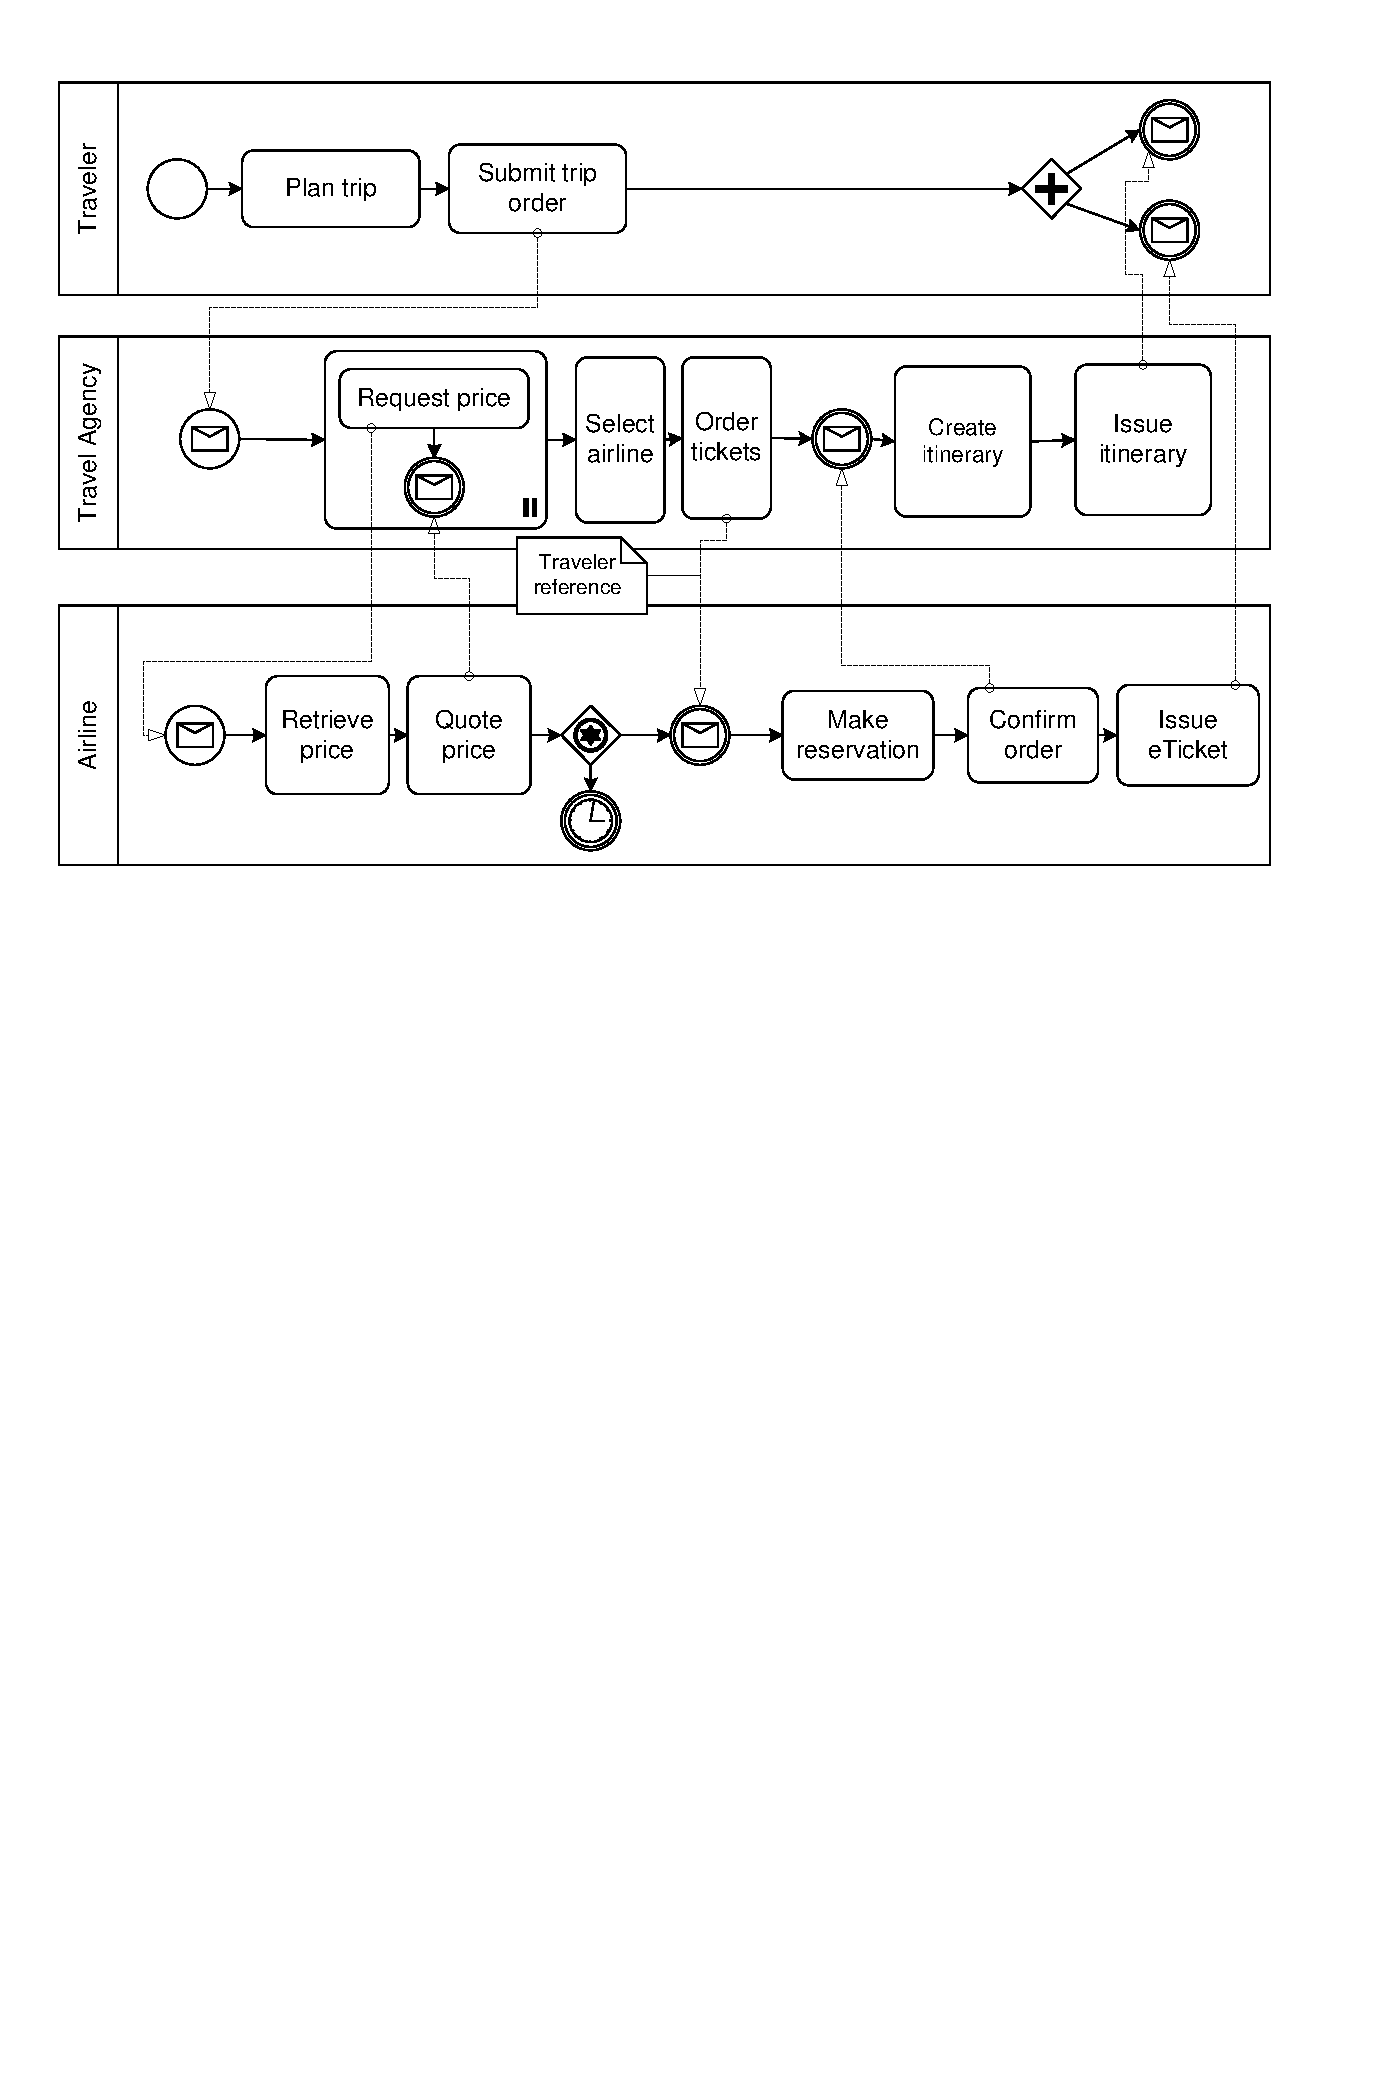
\includegraphics[width=\textwidth]{choreography.pdf}
  \caption{Beispiel-Choreographie I}
  \label{fig:AnhangsChor}
\end{figure}

\begin{landscape}
  %sidewaysfigure
  \begin{figure}
    \centering
    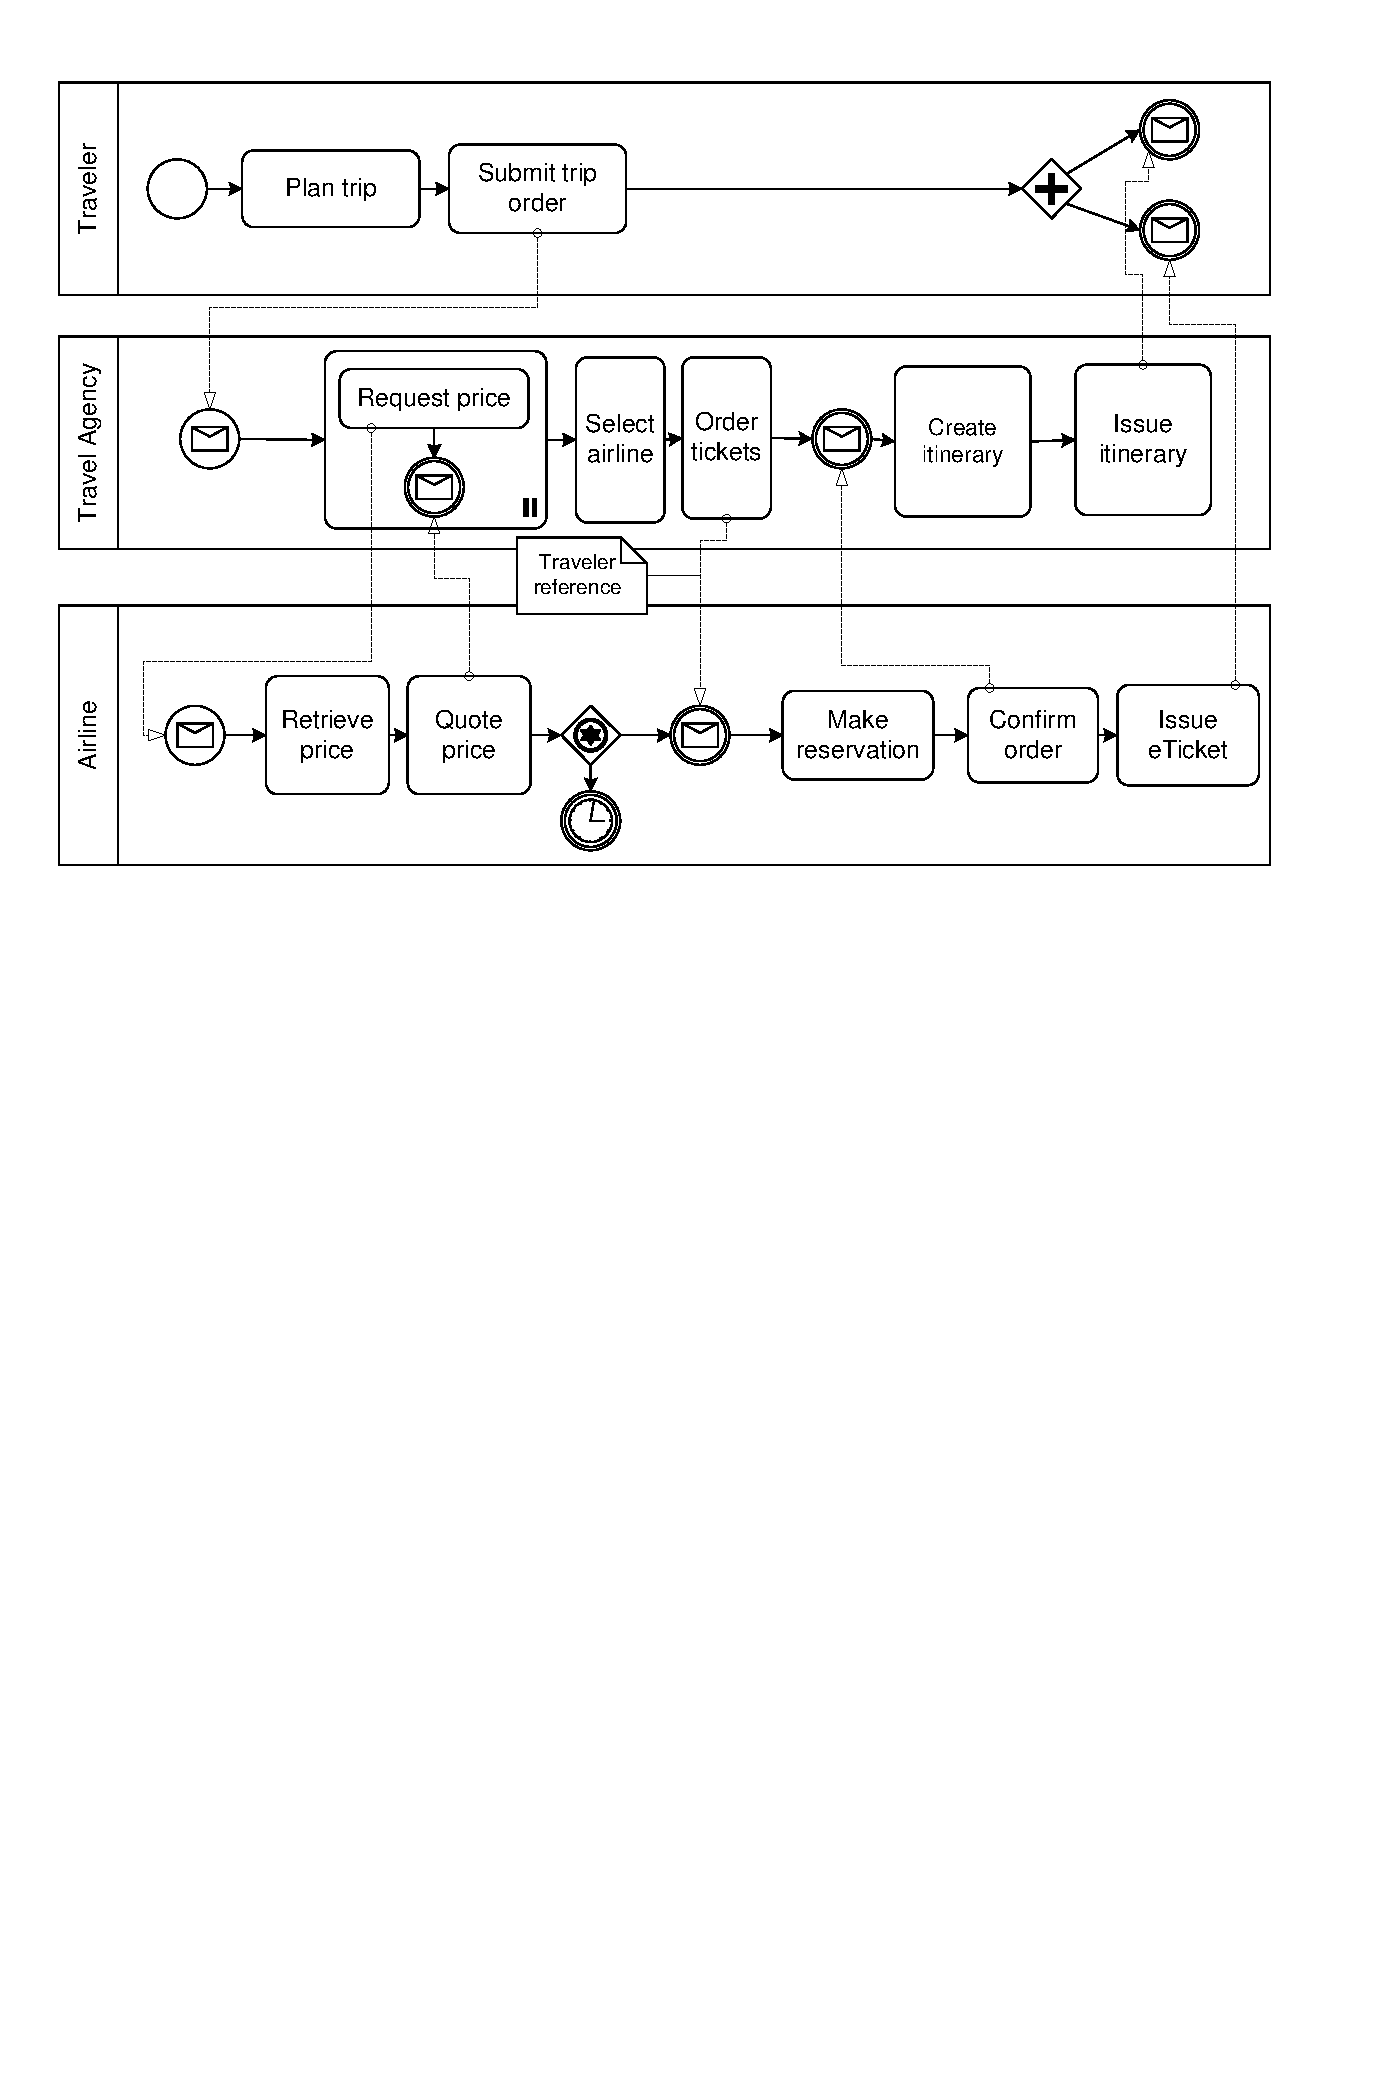
\includegraphics[width=\textwidth]{choreography.pdf}
    \caption{Beispiel-Choreographie II}
    \label{fig:AnhangsChor2}
  \end{figure}
\end{landscape}

\clearpage
%hint by http://tex.stackexchange.com/a/3265/9075
%other option is to use changepage according to http://tex.stackexchange.com/a/2639/9075. This, however, has issues with landscape
\thispagestyle{empty}

\savegeometry{koma}

%If you only have height problems, this is not needed at all
\addtolength{\textwidth}{2cm}
\addtolength{\evensidemargin}{-1cm}

\begin{landscape}
  %sidewaysfigure
  \begin{figure}
    \center
    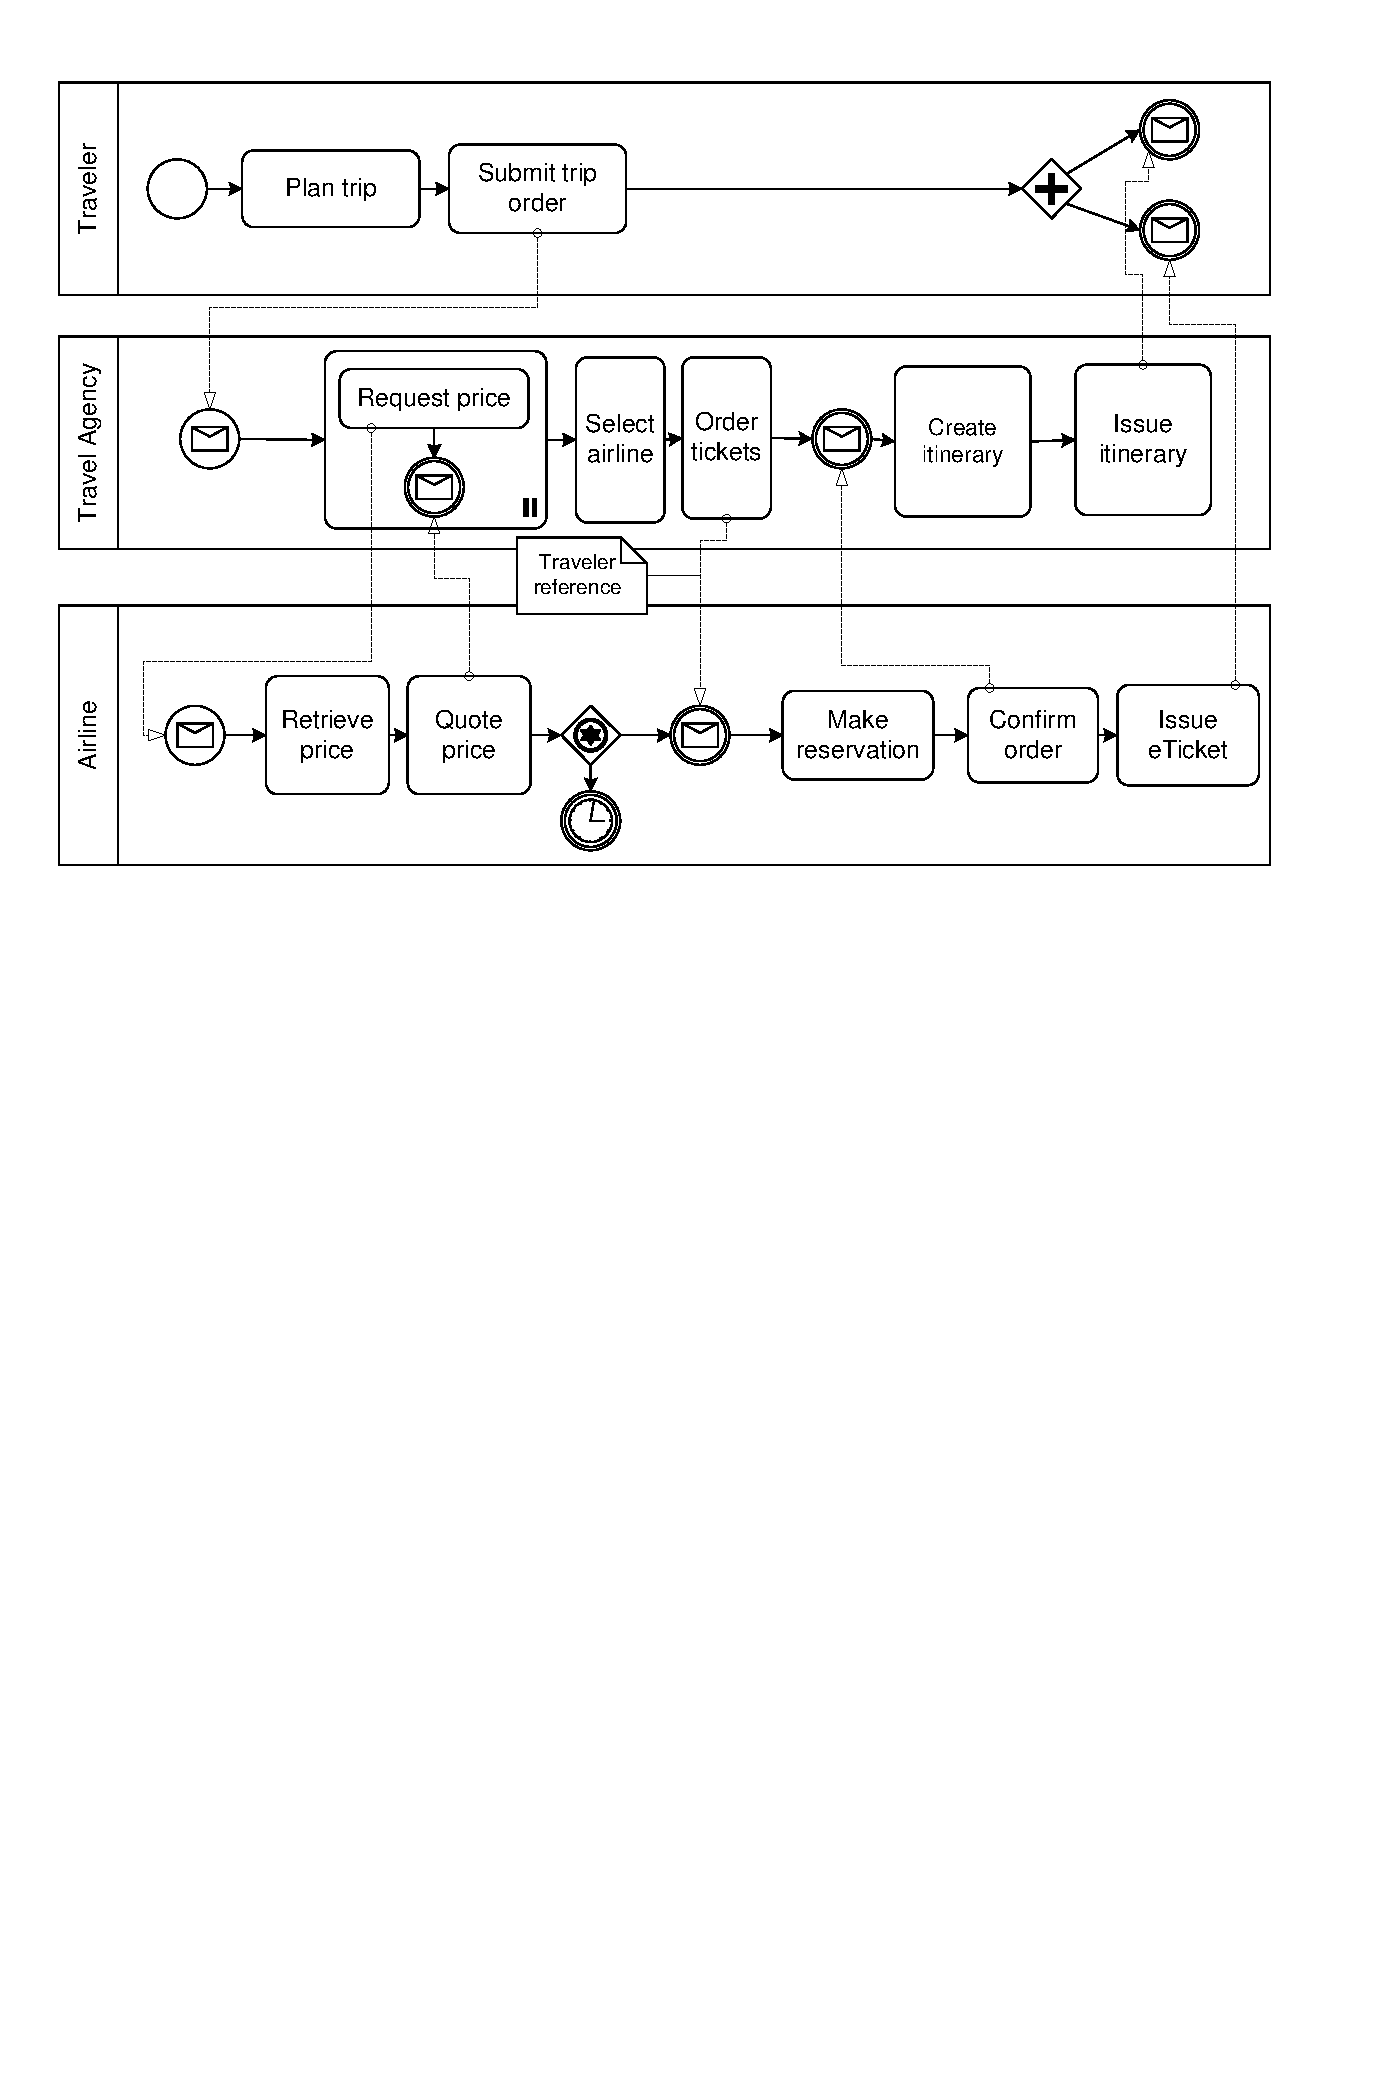
\includegraphics[width=0.9\paperheight]{choreography.pdf}
    \caption{Beispiel-Choreographie, auf einer weißen Seite gezeigt wird und über die definierten Seitenränder herausragt}
  \end{figure}
\end{landscape}

%the original layout is restored.
%%\restoregeometry cannot be used as we use \addtolength
\loadgeometry{koma}

\section{Schlusswort}
Verbesserungsvorschläge für diese Vorlage sind immer willkommen.
Bitte bei github ein Ticket eintragen (\url{https://github.com/latextemplates/uni-stuttgart-computer-science-template/issues}).

\section{Nachfolgerinfo}\label{chap:nachfolger}
\includepdf[pages=-]{preambel/Nachfolger-Info_Studienarbeit_autonome_Drohnen.pdf}

\clearpage

%\printindex

\printbibliography

%\ifdeutsch
%Alle URLs wurden zuletzt am 17.\,03.\,2008 geprüft.
%\else
%All links were last followed on March 17, 2008.
%\fi

\pagestyle{empty}
\renewcommand*{\chapterpagestyle}{empty}
\Versicherung
\end{document}
